\appendix

\chapter{\textit{Hyperparameter} pelatihan}

\begin{table}[h]
    \centering
    \caption{\textit{Hyperparameter} pelatihan}
    \label{appendix:hyperparameter-train}
    \resizebox{\textwidth}{!}{
        \begin{tabular}{|c|l|c|}
            \hline 
            \textbf{Tugas} & \multicolumn{1}{|c|}{\textbf{Argumen}} & \textbf{Nilai} \\ \hline
            \multirow{9}{*}{\textit{NER}} & \texttt{model} & "indolem/indobert-base-uncased" \\ \cline{2-3}
                                          & \texttt{train\_batch\_size} & 16 \\ \cline{2-3}
                                          & \texttt{eval\_batch\_size} & 64 \\ \cline{2-3}
                                          & \texttt{epochs} & 100 \\ \cline{2-3}
                                          & \texttt{learning\_rate} & 5e-5 \\ \cline{2-3}
                                          & \texttt{max\_sequence\_length} & 128 \\ \cline{2-3}
                                          & \texttt{text\_column\_names} & "tokens" \\ \cline{2-3}
                                          & \texttt{label\_column\_names} & "ner\_tags" \\ \cline{2-3}
                                          & \texttt{return\_entity\_level\_metrics} & true \\ \cline{2-3}
                                          & \texttt{seed} & 42 \\ \hline
            \multirow{7}{*}{\textit{Sentiment Analysis}} & \texttt{model} & "indolem/indobert-base-uncased" \\ \cline{2-3}
                                                         & \texttt{batch\_size} & 30 \\ \cline{2-3}
                                                         & \texttt{epochs} & 20 \\ \cline{2-3}
                                                         & \texttt{learning\_rate} & 5e-5 \\ \cline{2-3}
                                                         & \texttt{max\_sequence\_length} & 200 \\ \cline{2-3}
                                                         & \texttt{seed} & 42 \\ \cline{2-3}
                                                         & \texttt{label\_names} & "labels" \\ \hline
            \multirow{14}{*}{\textit{Summarization}} & \texttt{model} & "lazarusnlp/indonanot5-base" \\ \cline{2-3}
                                                    & \texttt{train\_batch\_size} & 4 \\ \cline{2-3}
                                                    & \texttt{eval\_batch\_size} & 8 \\ \cline{2-3}
                                                    & \texttt{epochs} & 5 \\ \cline{2-3}
                                                    & \texttt{learning\_rate} & 1e-5 \\ \cline{2-3}
                                                    & \texttt{max\_source\_length} & 512 \\ \cline{2-3}
                                                    & \texttt{max\_target\_length} & 512 \\ \cline{2-3}
                                                    & \texttt{num\_beams} & 5 \\ \cline{2-3}
                                                    & \texttt{weight\_decay} & 0.01 \\ \cline{2-3}
                                                    & \texttt{patience} & 5 \\ \cline{2-3}
                                                    & \texttt{seed} & 42 \\ \cline{2-3}
                                                    & \texttt{text\_column} & paragraphs \\ \cline{2-3}
                                                    & \texttt{summary\_column} & summary \\ \cline{2-3}
                                                    & \texttt{source\_prefix} & "summarize: " \\ \cline{2-3}
                                                    & \texttt{pad\_to\_max\_length} & true \\ \cline{2-3}
                                                    & \texttt{predict\_with\_generate} & true \\ \cline{2-3}
                                                    & \texttt{bf16} & true \\ \hline
        \end{tabular}
    }
\end{table}

\chapter{Hasil Evaluasi dan Prediksi Tugas NER pada NER UI}
\label{appendix:nerui}

\begin{figure}[h]
    \centering
    \begin{longtable}{c}
        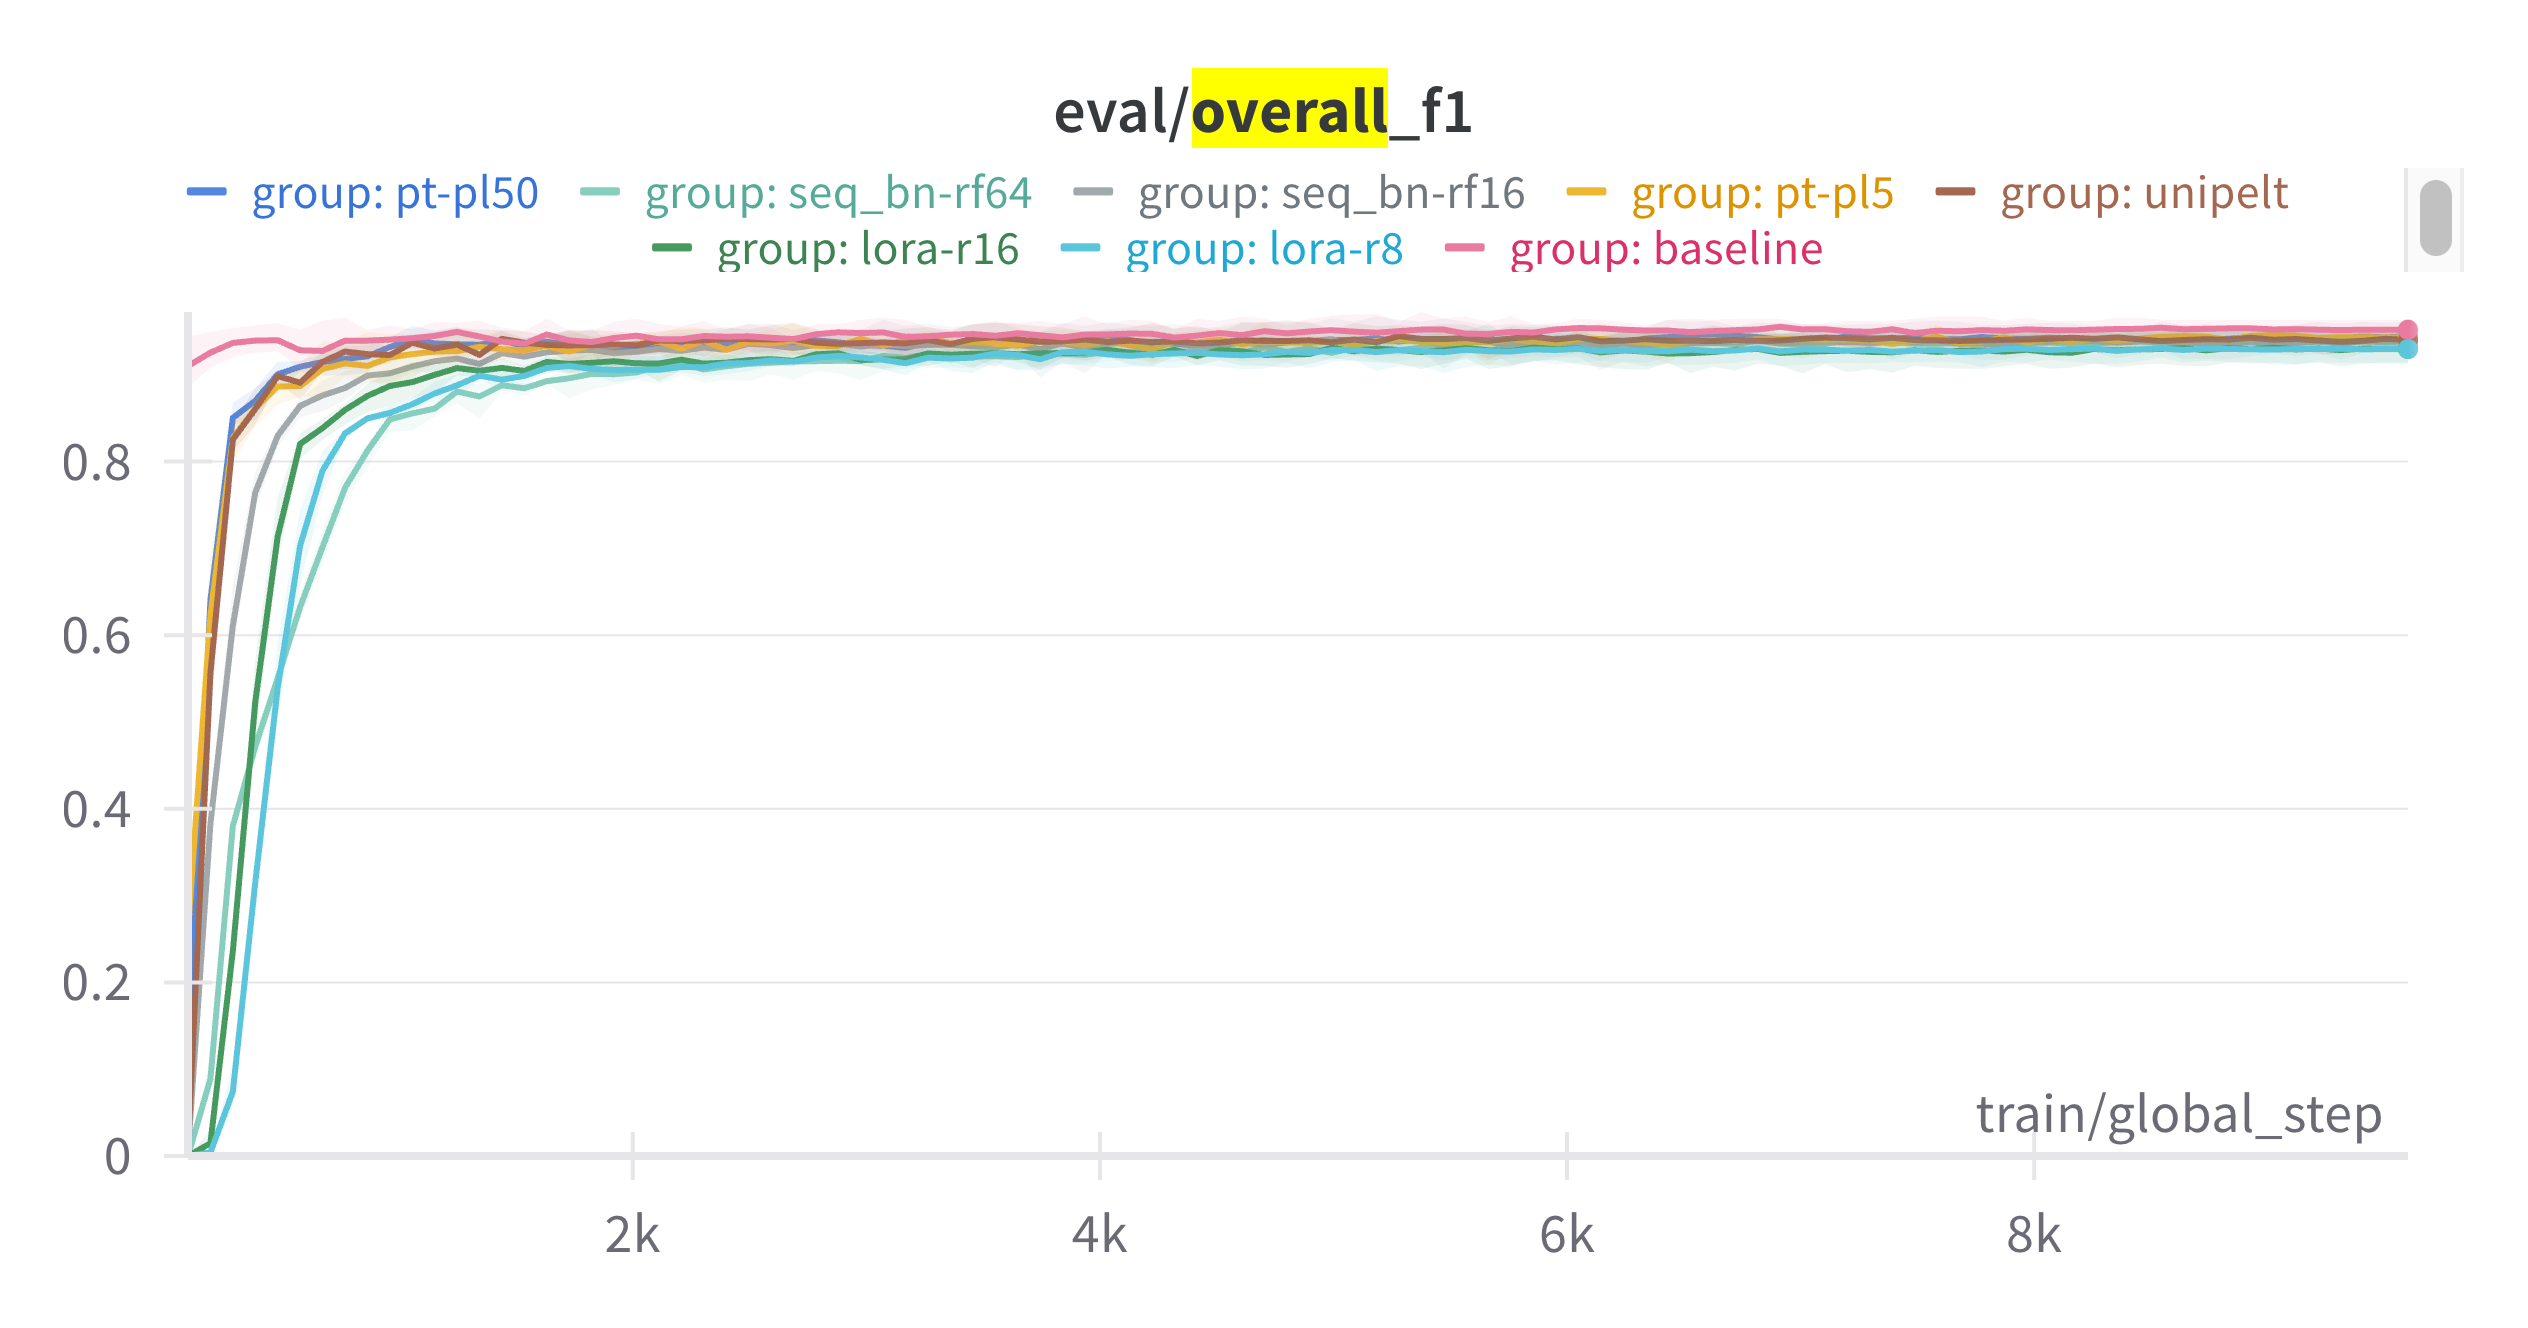
\includegraphics[width=\textwidth]{appendix/nerui_eval_f1.png} \\
        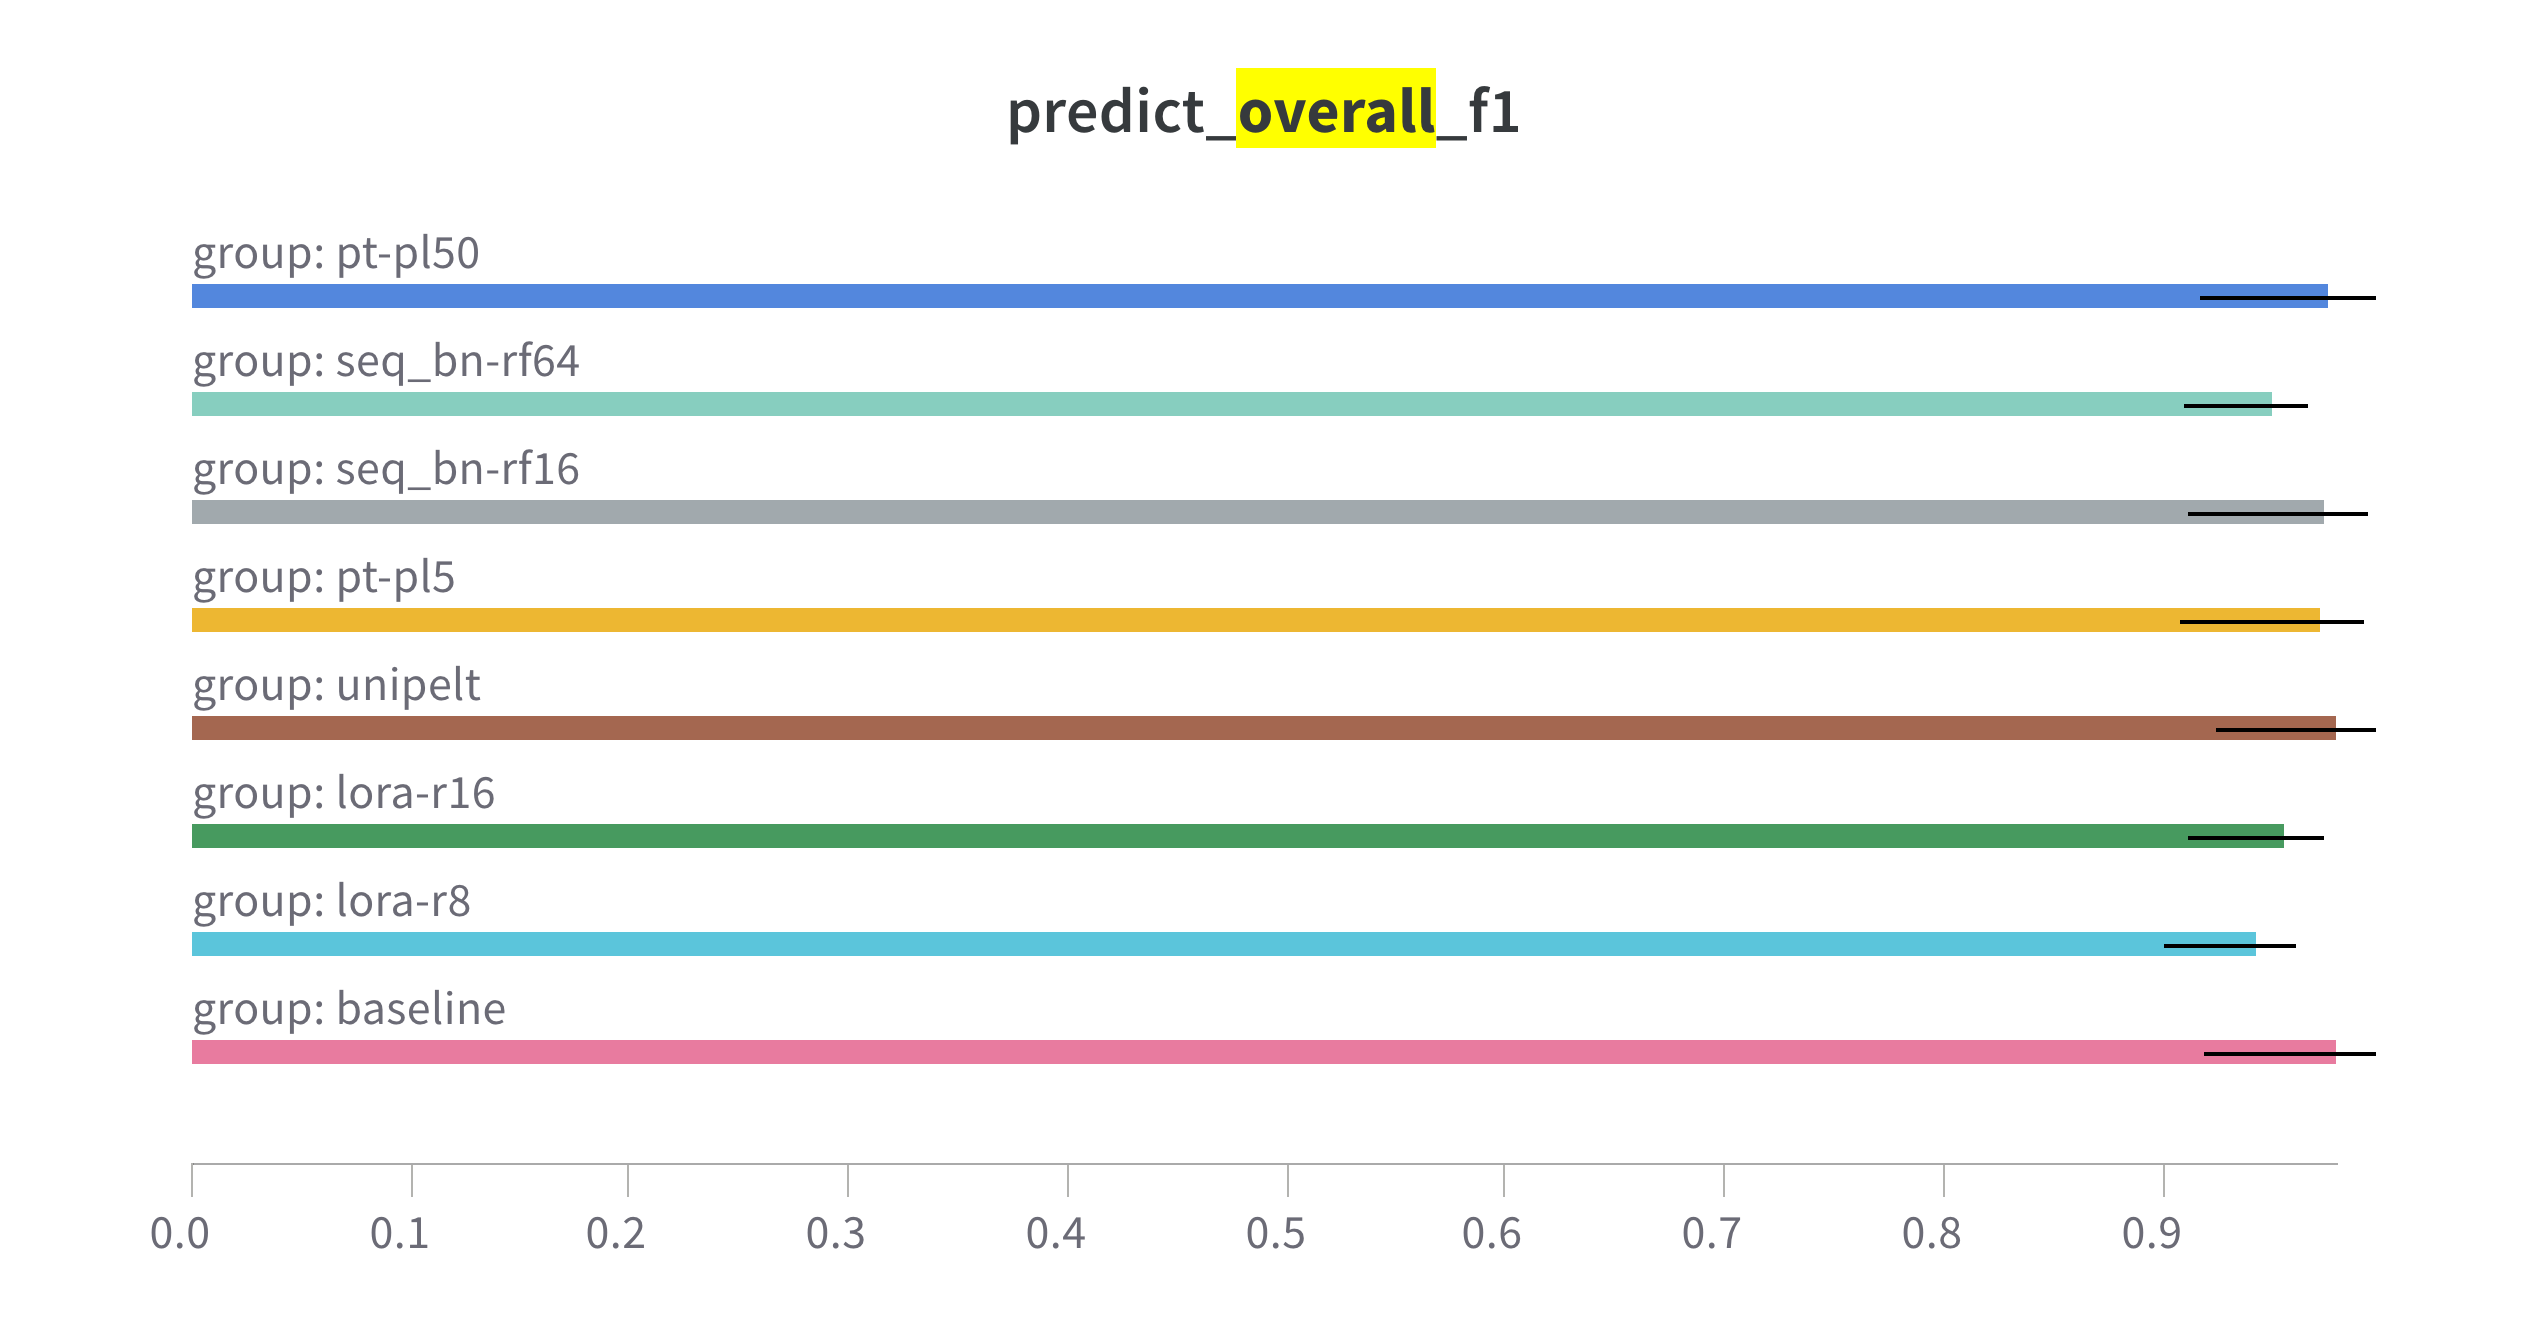
\includegraphics[width=\textwidth]{appendix/nerui_pred_f1.png} \\
    \end{longtable}
    \caption{Hasil evaluasi dan prediksi F1 tugas NER pada NER UI}
\end{figure}

\begin{figure}[h]
    \centering
    \begin{longtable}{c}
        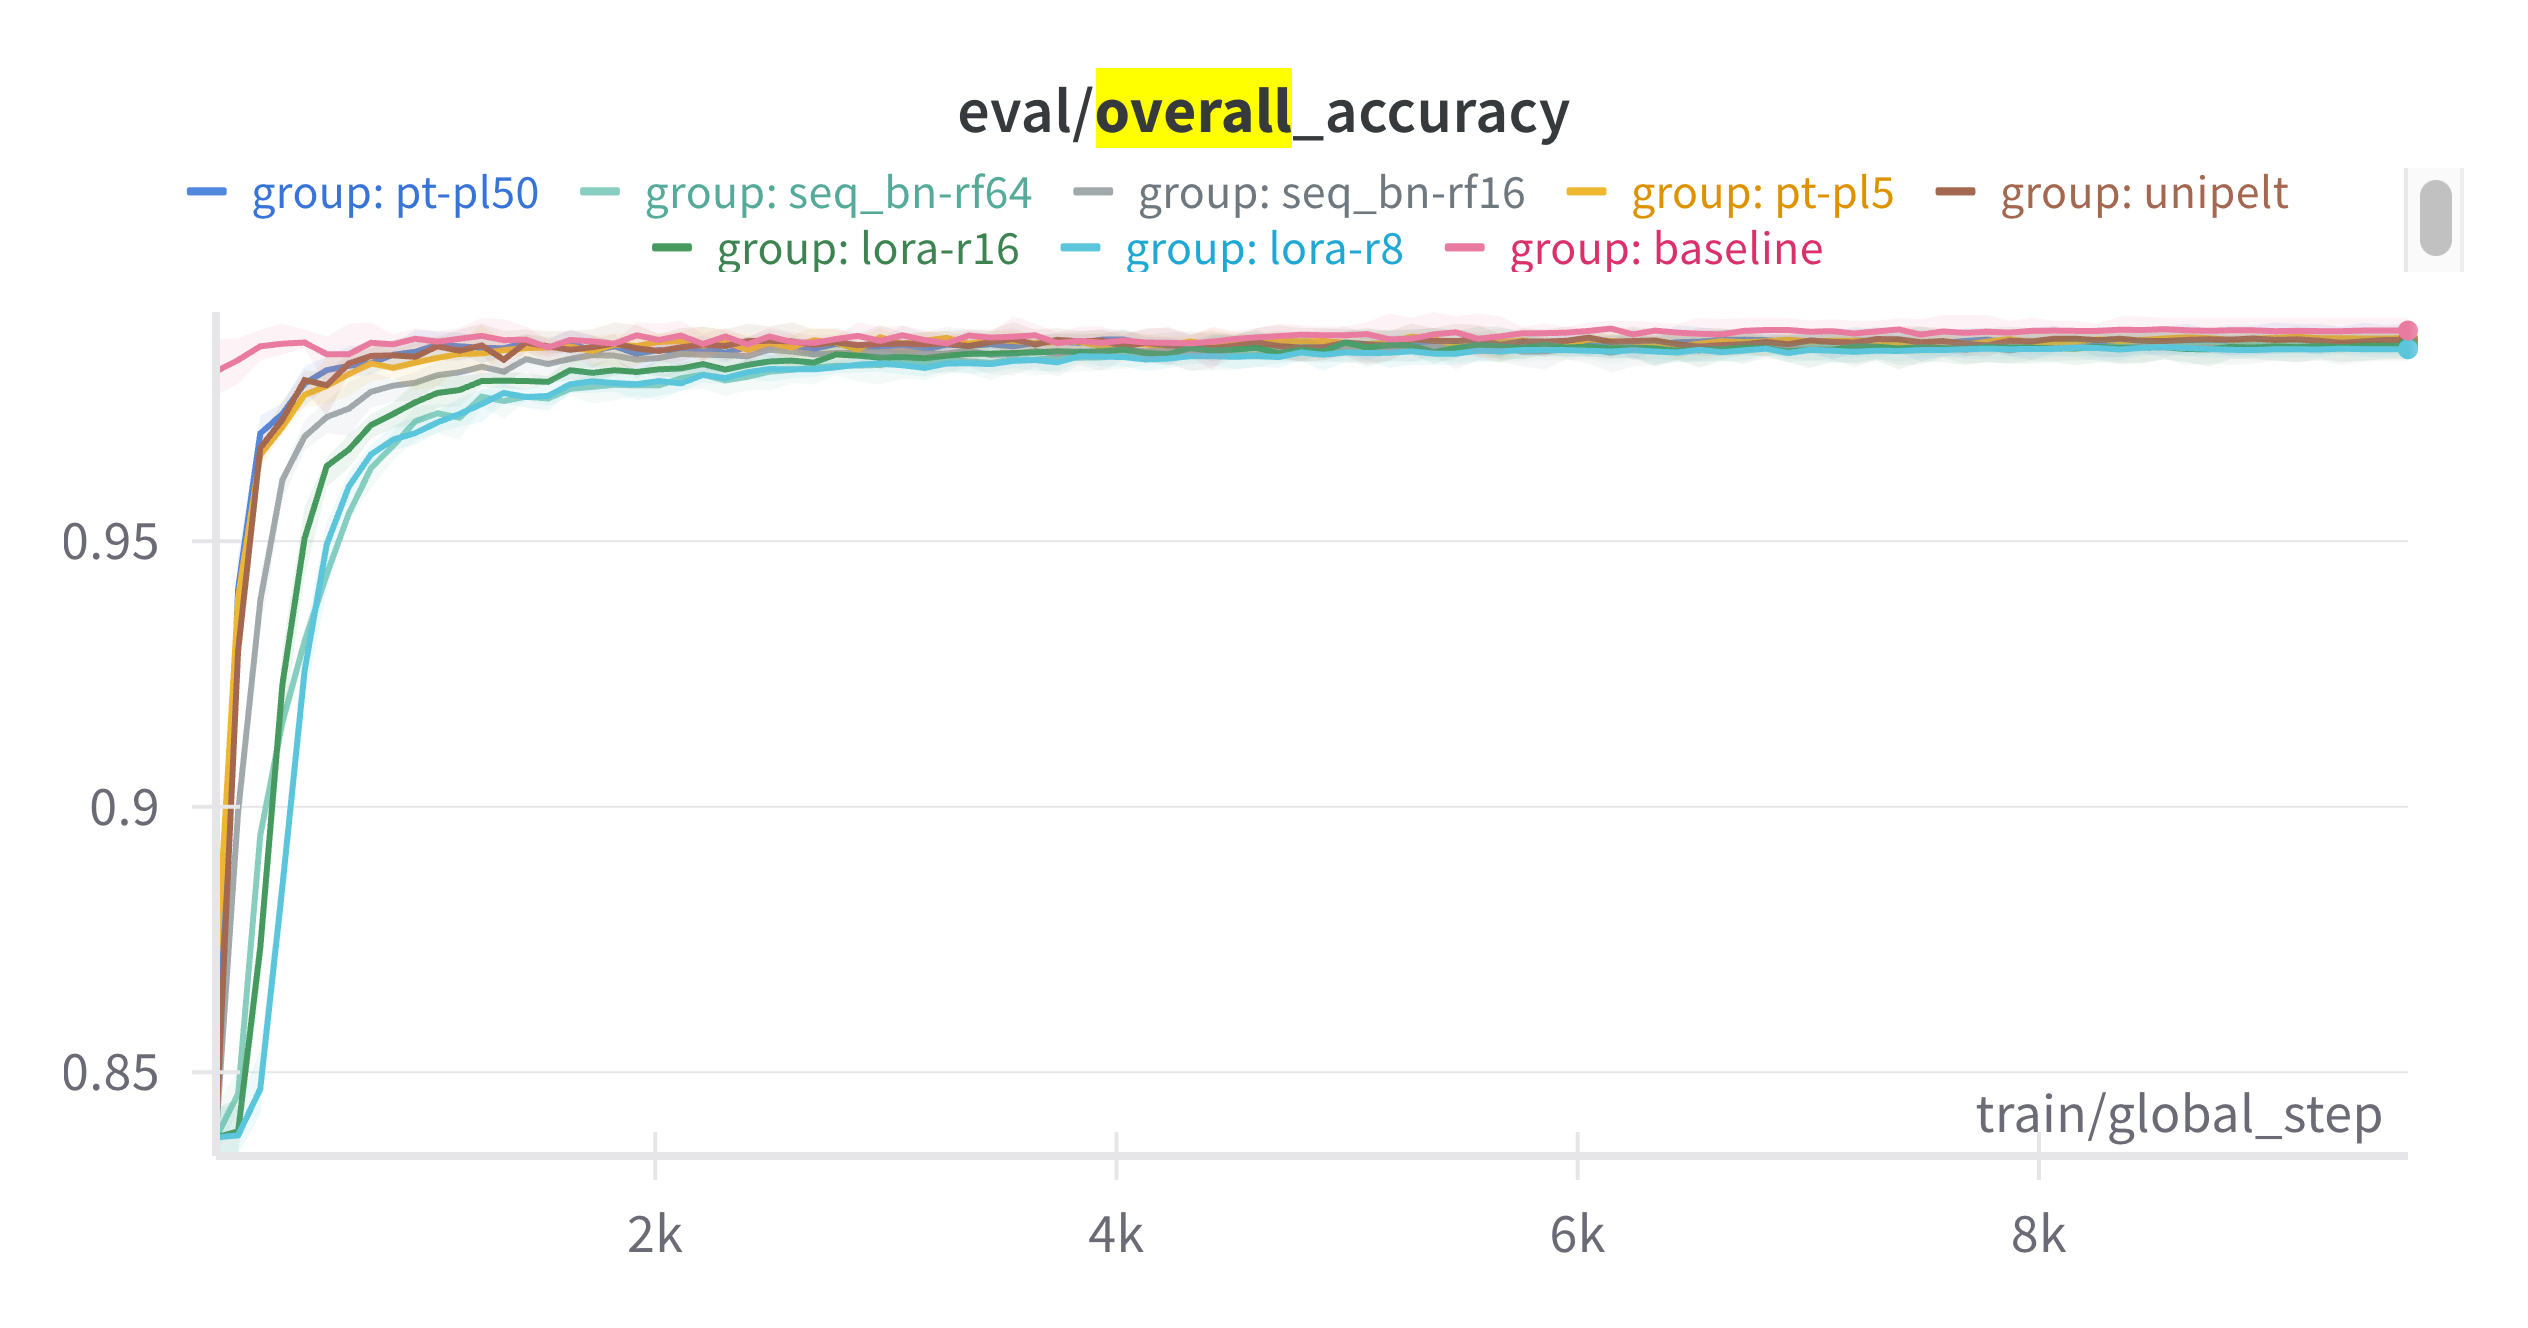
\includegraphics[width=\textwidth]{appendix/nerui_eval_acc.png} \\
        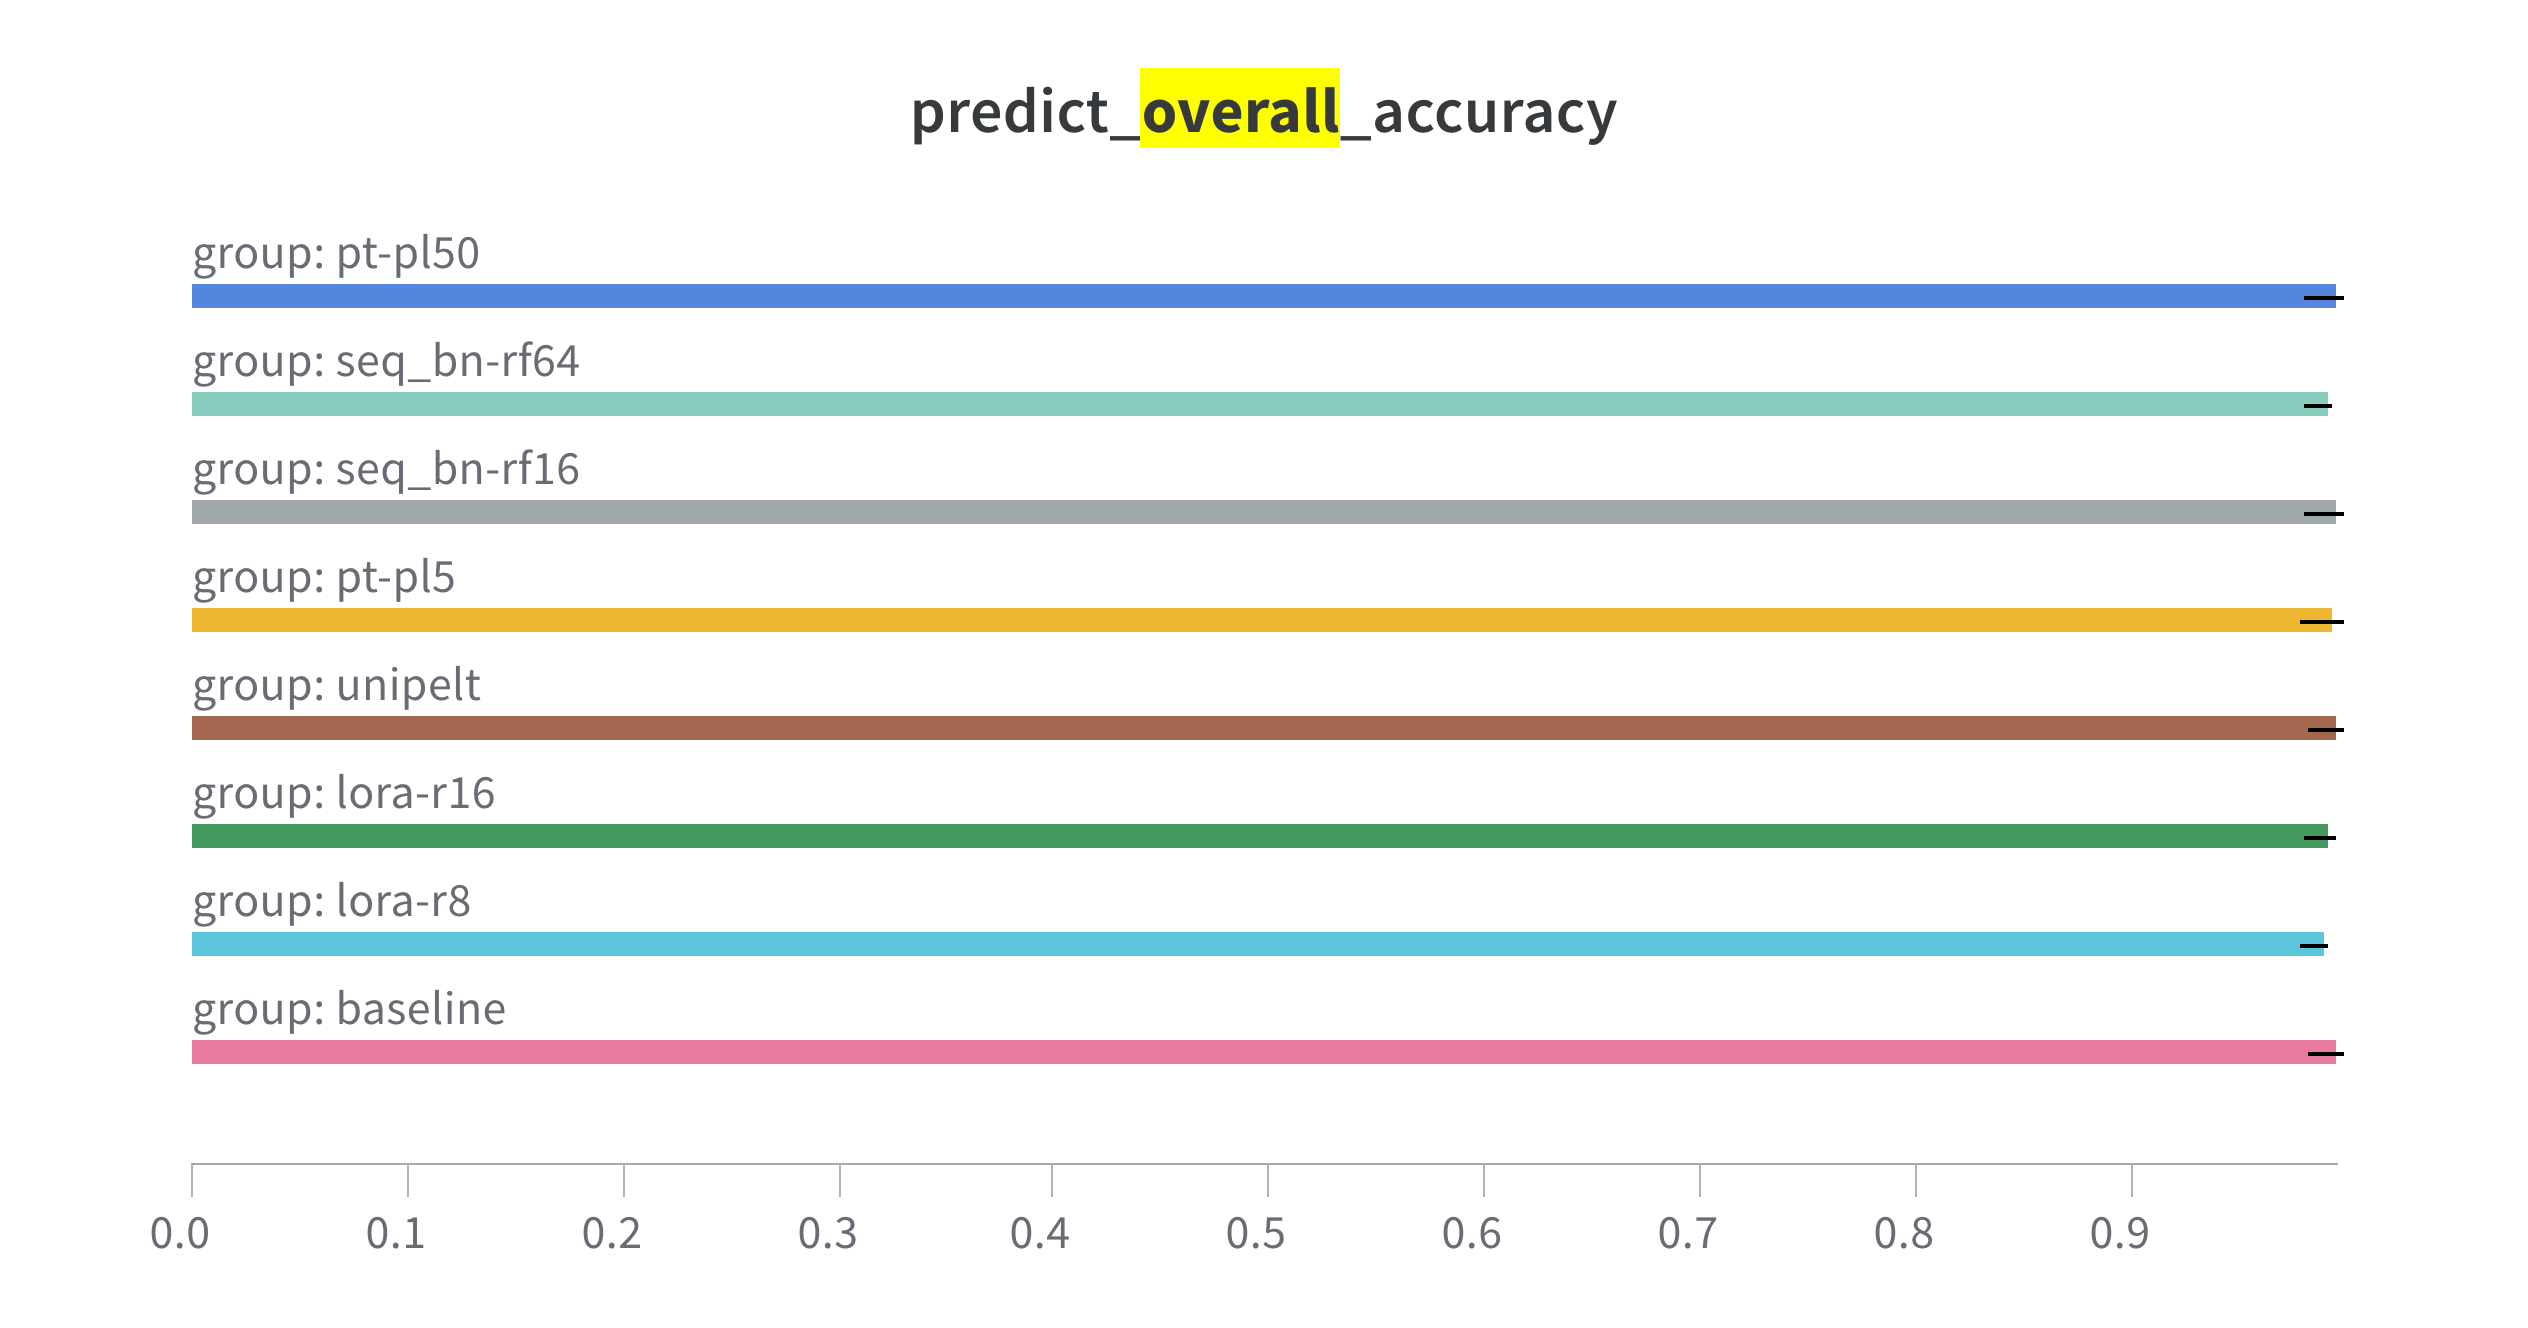
\includegraphics[width=\textwidth]{appendix/nerui_pred_acc.png} \\
    \end{longtable}
    \caption{Hasil evaluasi dan prediksi \textit{accuracy} tugas NER pada NER UI}
\end{figure}

\begin{figure}[h]
    \centering
    \begin{longtable}{c}
        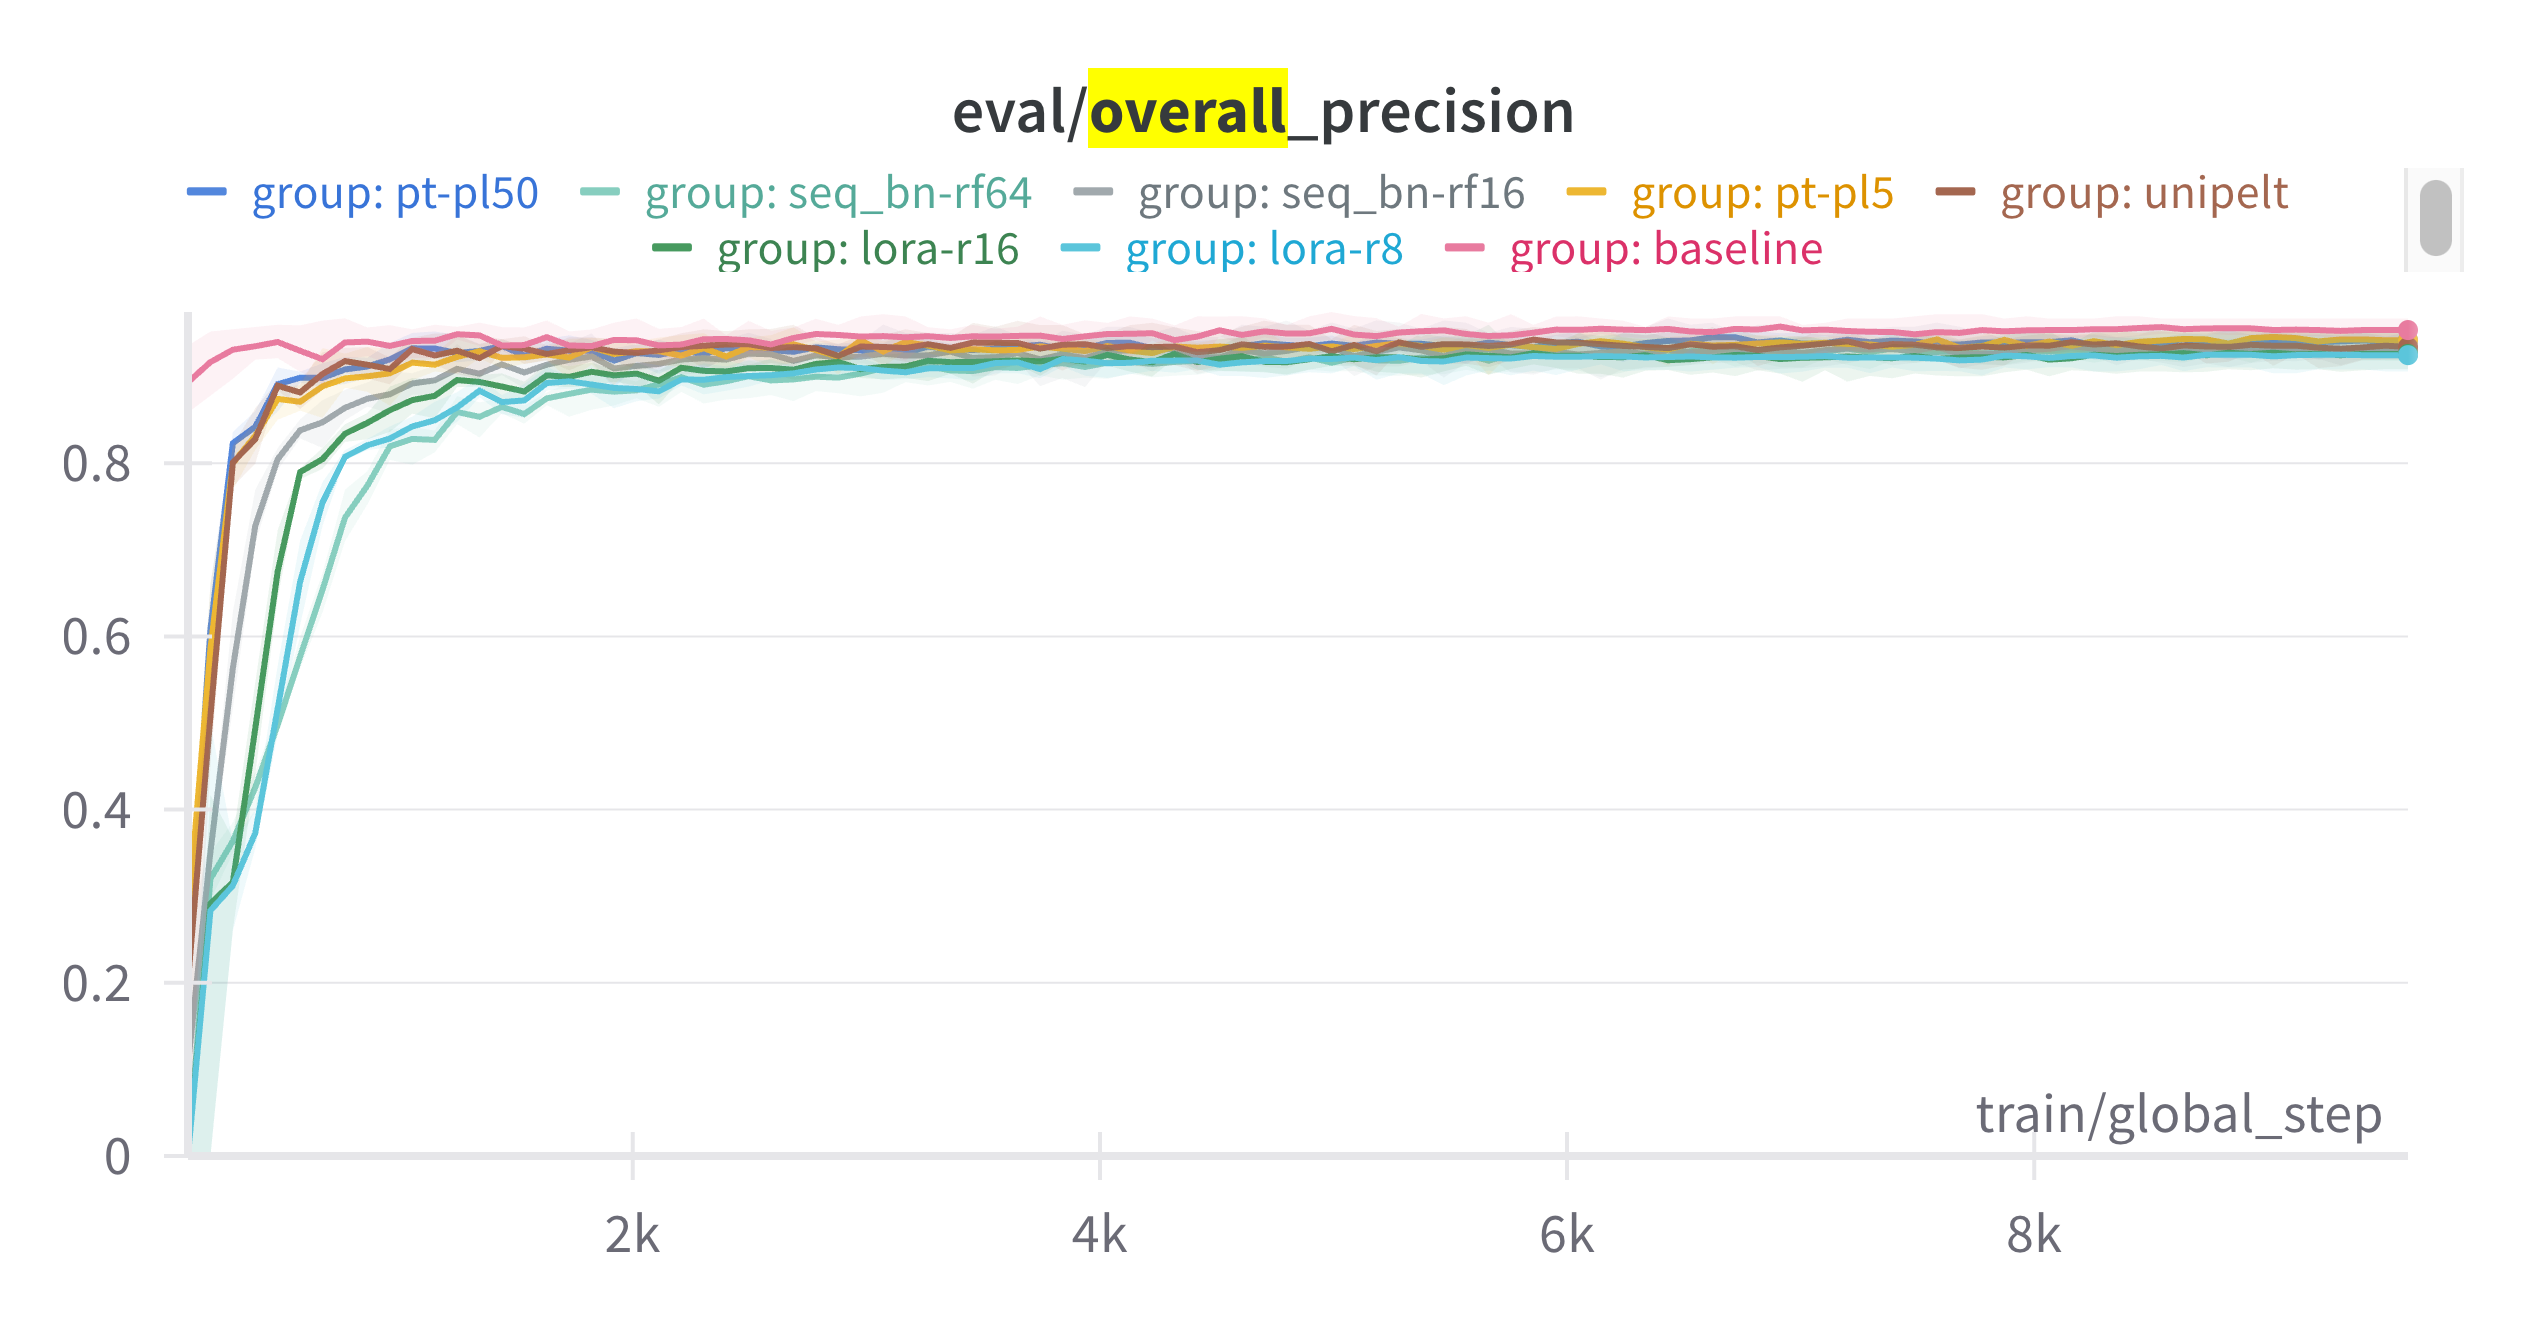
\includegraphics[width=\textwidth]{appendix/nerui_eval_precision.png} \\
        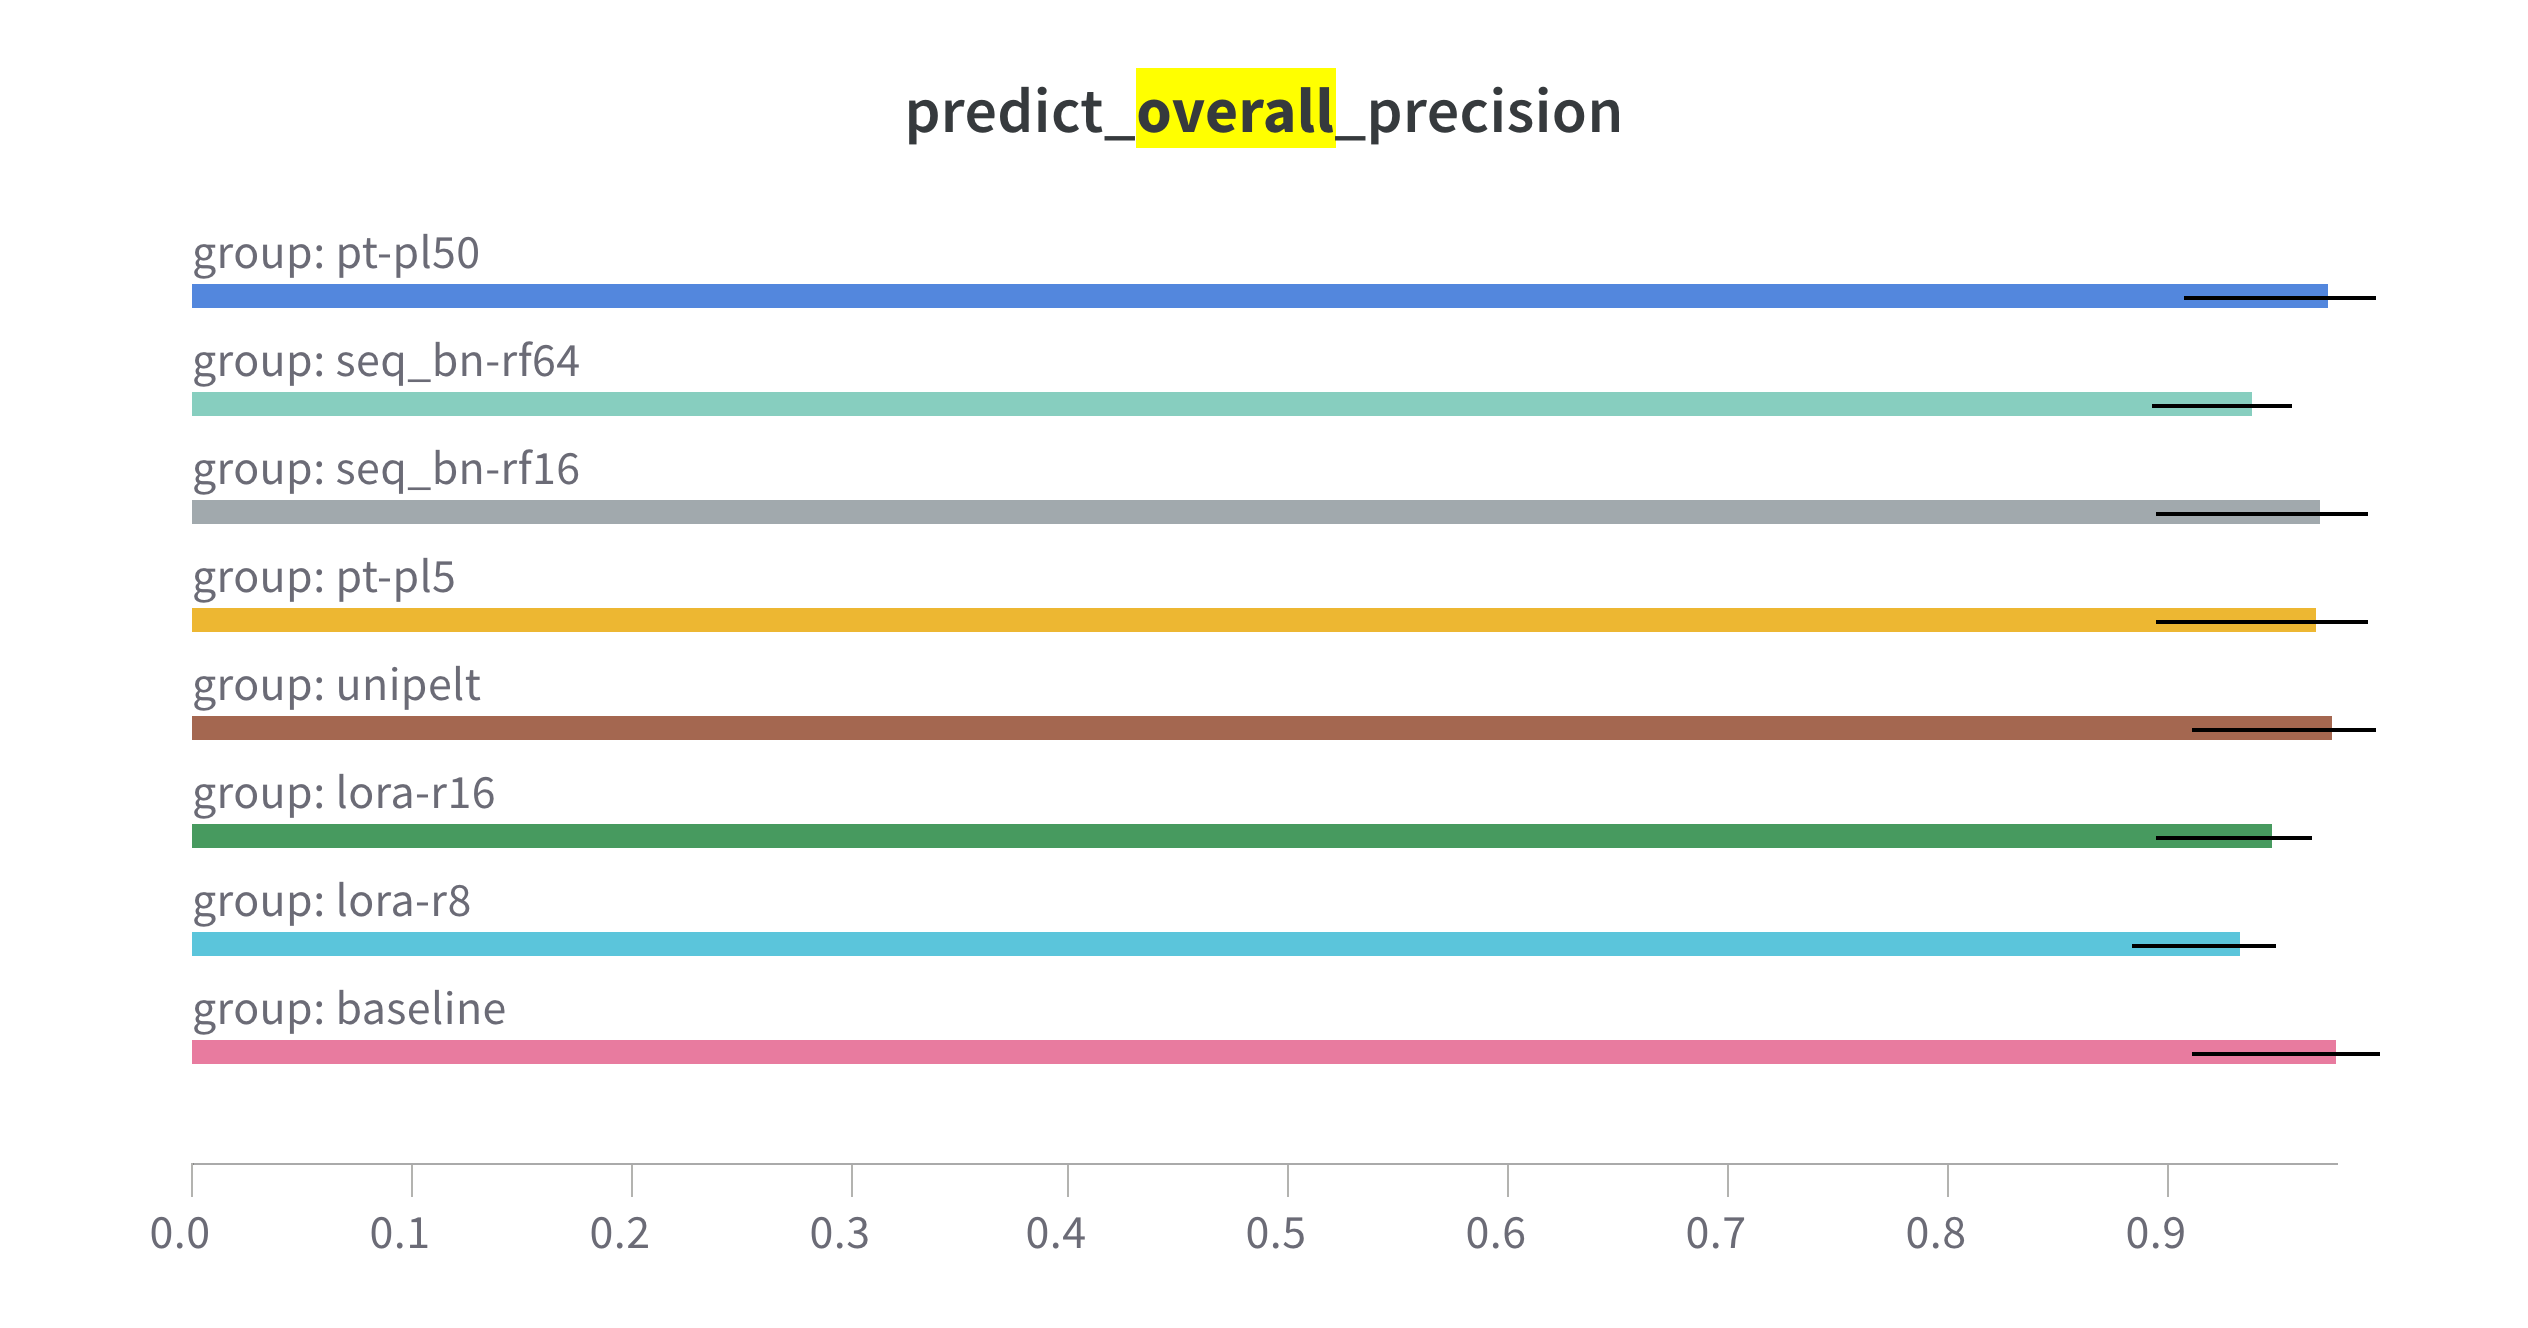
\includegraphics[width=\textwidth]{appendix/nerui_pred_precision.png} \\
    \end{longtable}
    \caption{Hasil evaluasi dan prediksi \textit{precision} tugas NER pada NER UI}
\end{figure}

\begin{figure}[h]
    \centering
    \begin{longtable}{c}
        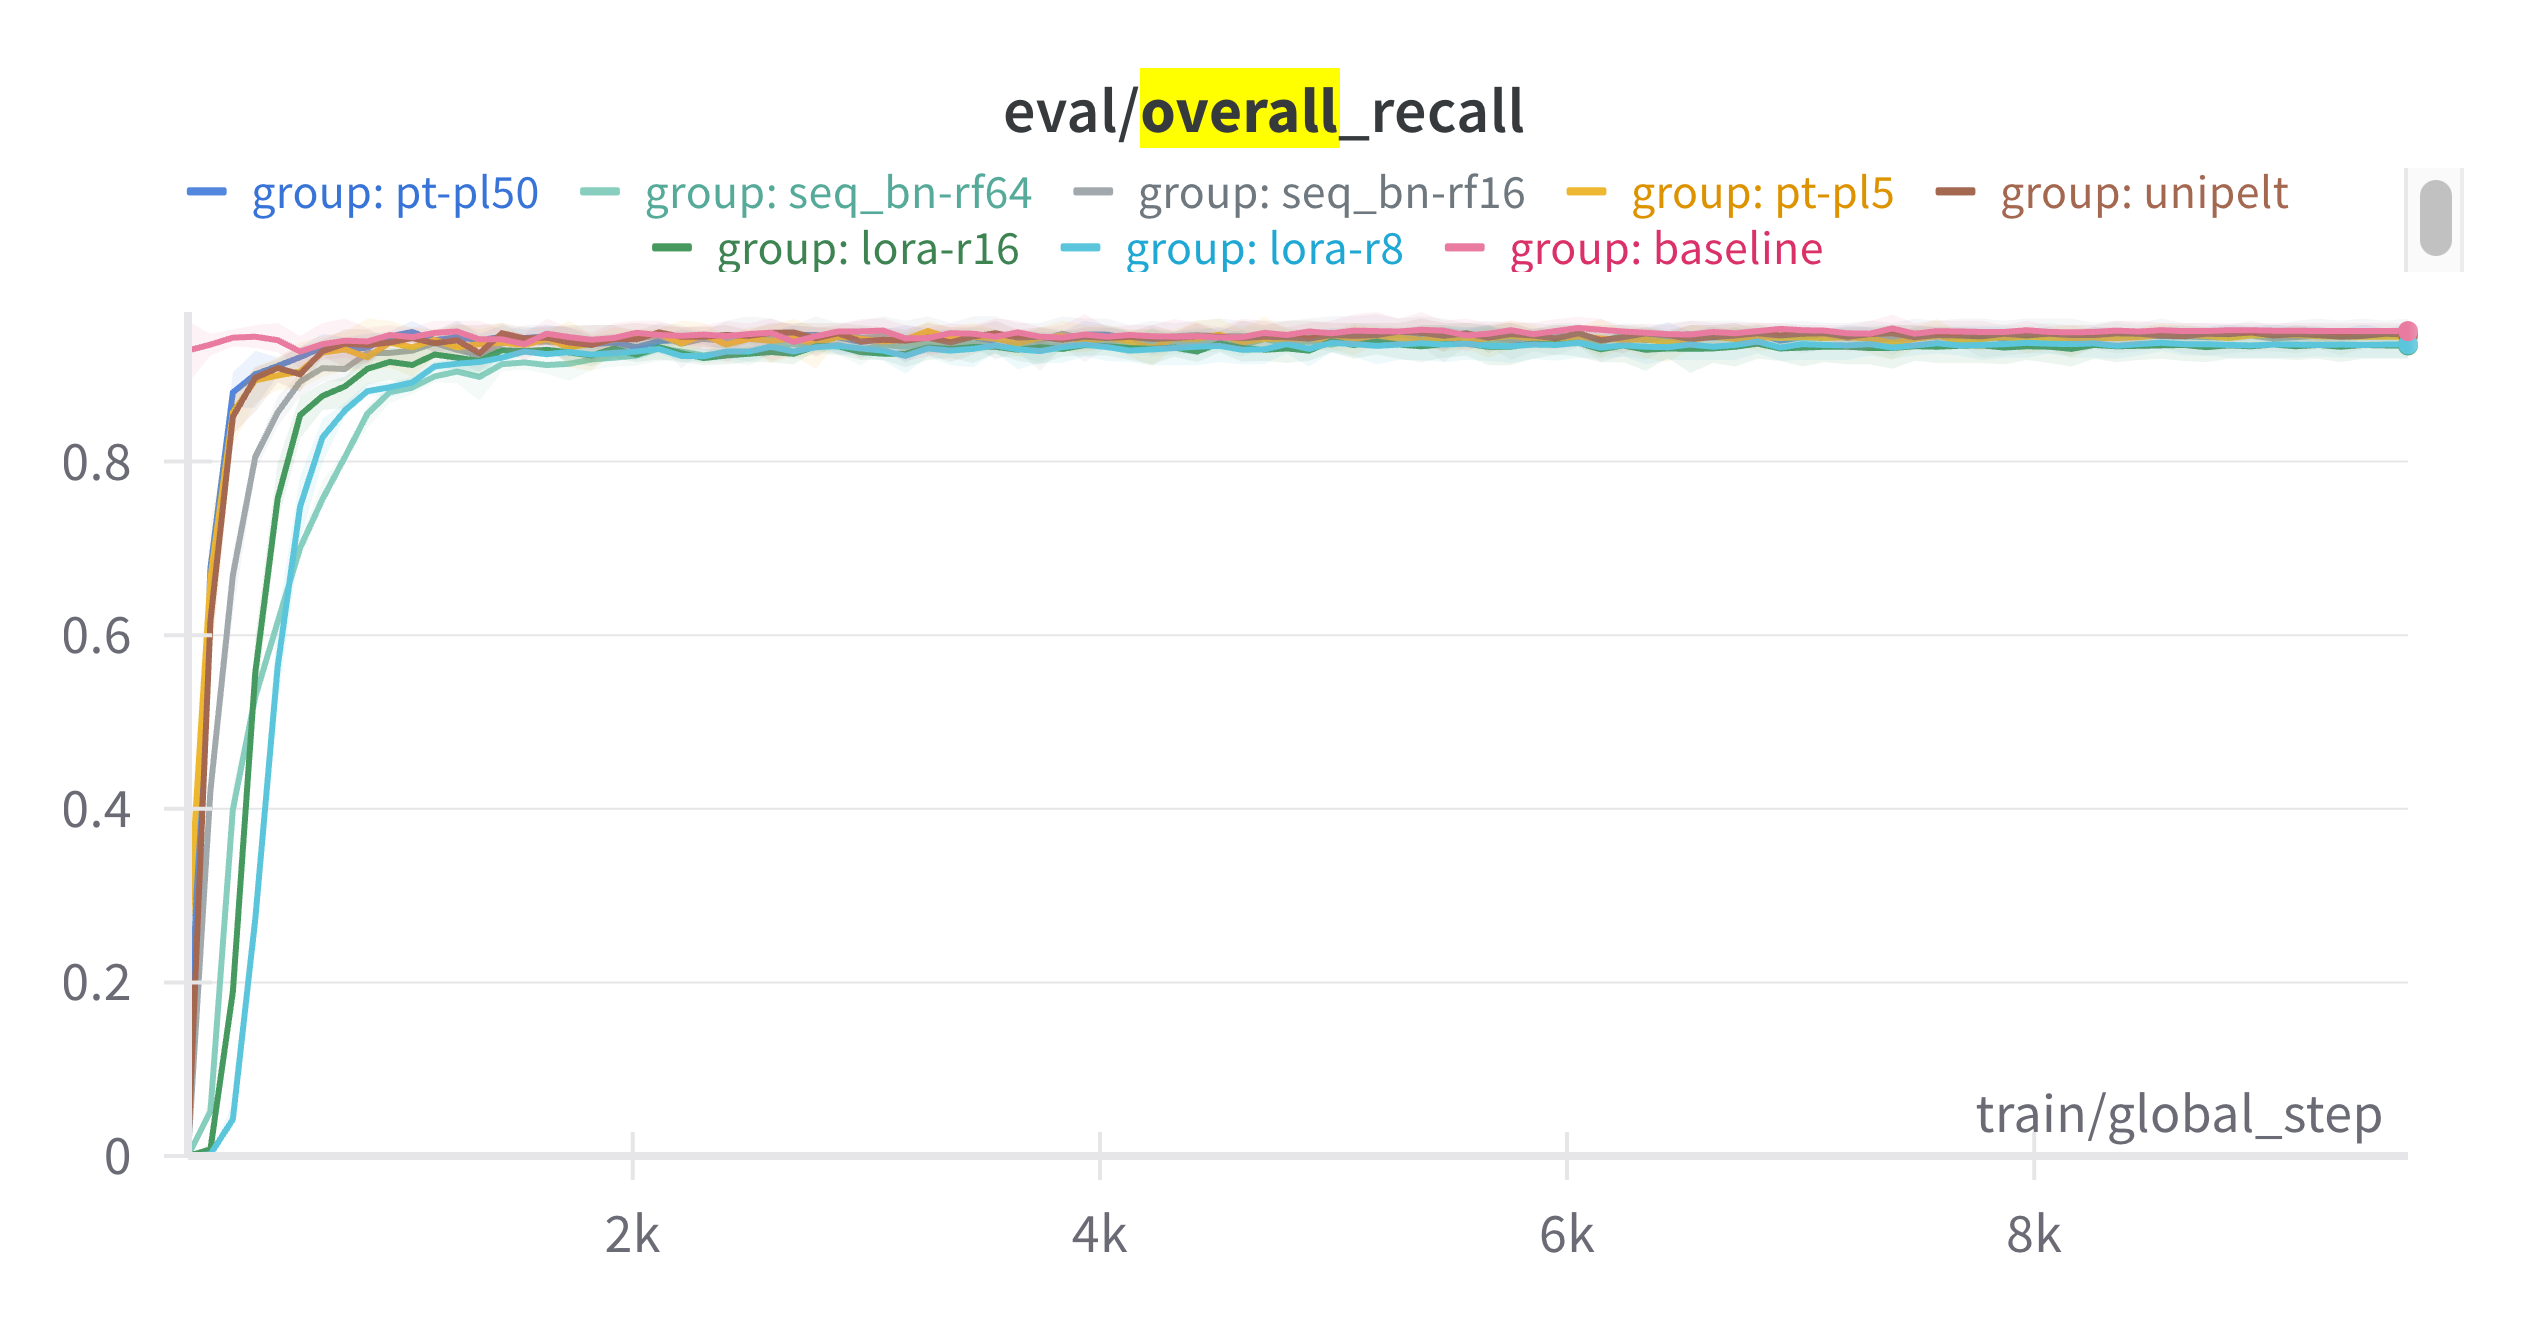
\includegraphics[width=\textwidth]{appendix/nerui_eval_recall.png} \\
        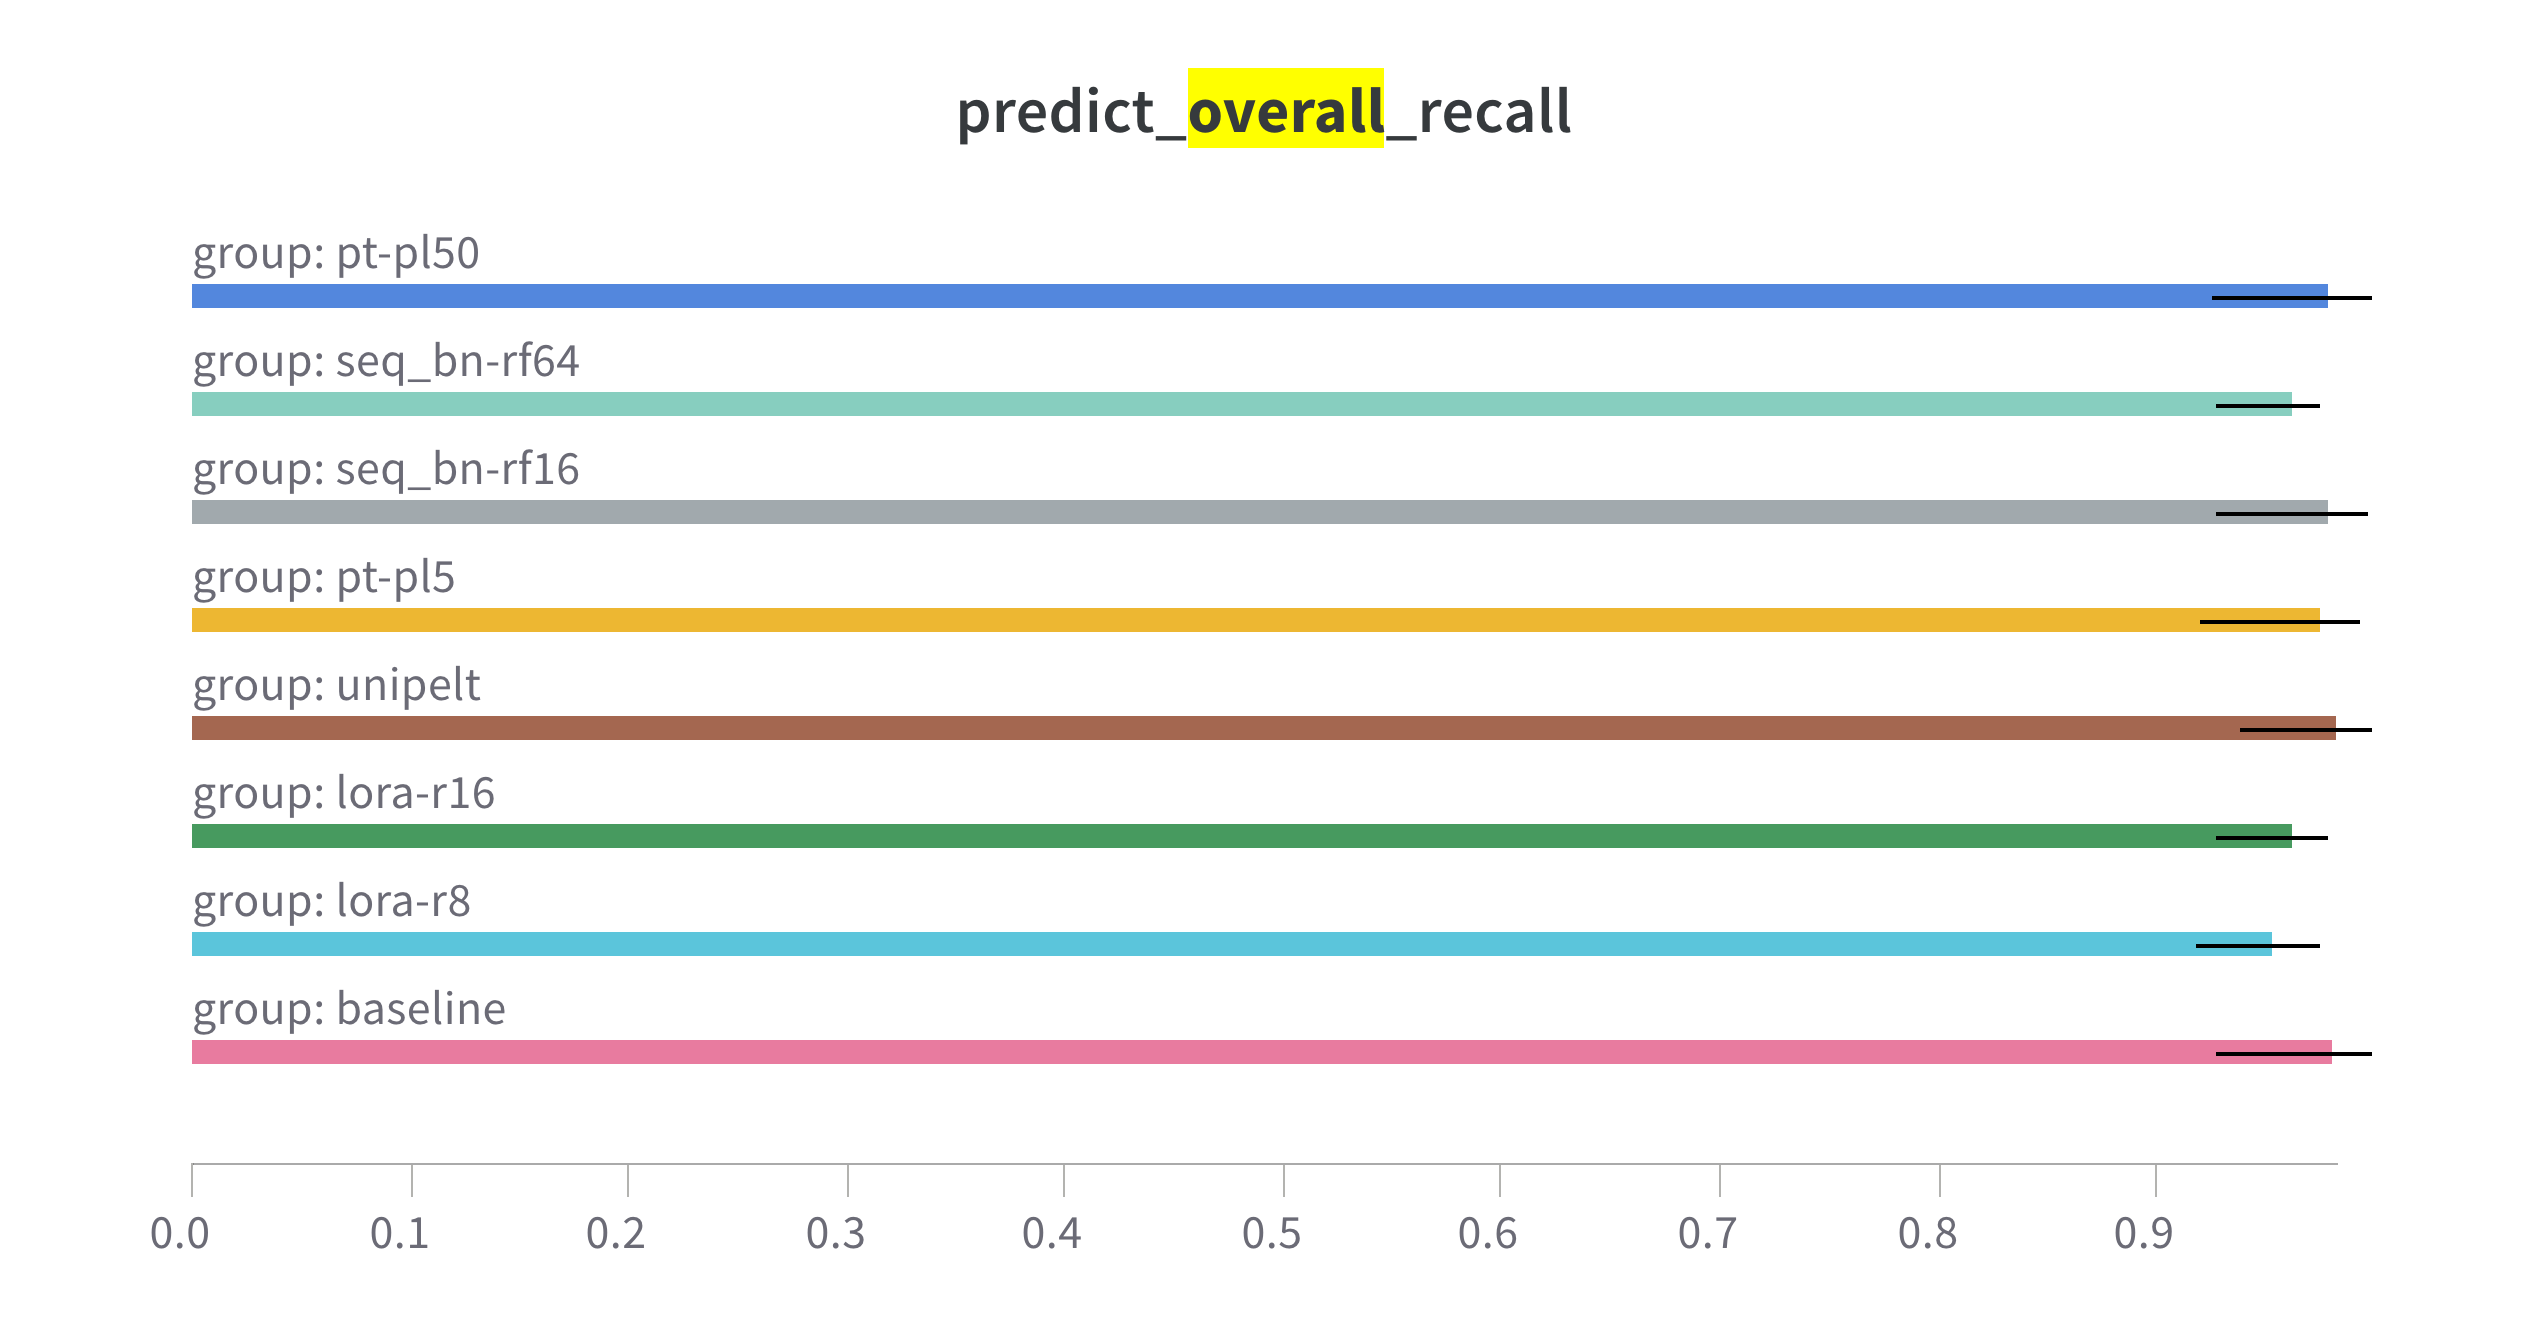
\includegraphics[width=\textwidth]{appendix/nerui_pred_recall.png} \\
    \end{longtable}
    \caption{Hasil evaluasi dan prediksi \textit{recall} tugas NER pada NER UI}
\end{figure}

\chapter{Hasil Evaluasi dan Prediksi Tugas NER pada NER UGM}
\label{appendix:nerugm}

\begin{figure}[h]
    \centering
    \begin{longtable}{c}
        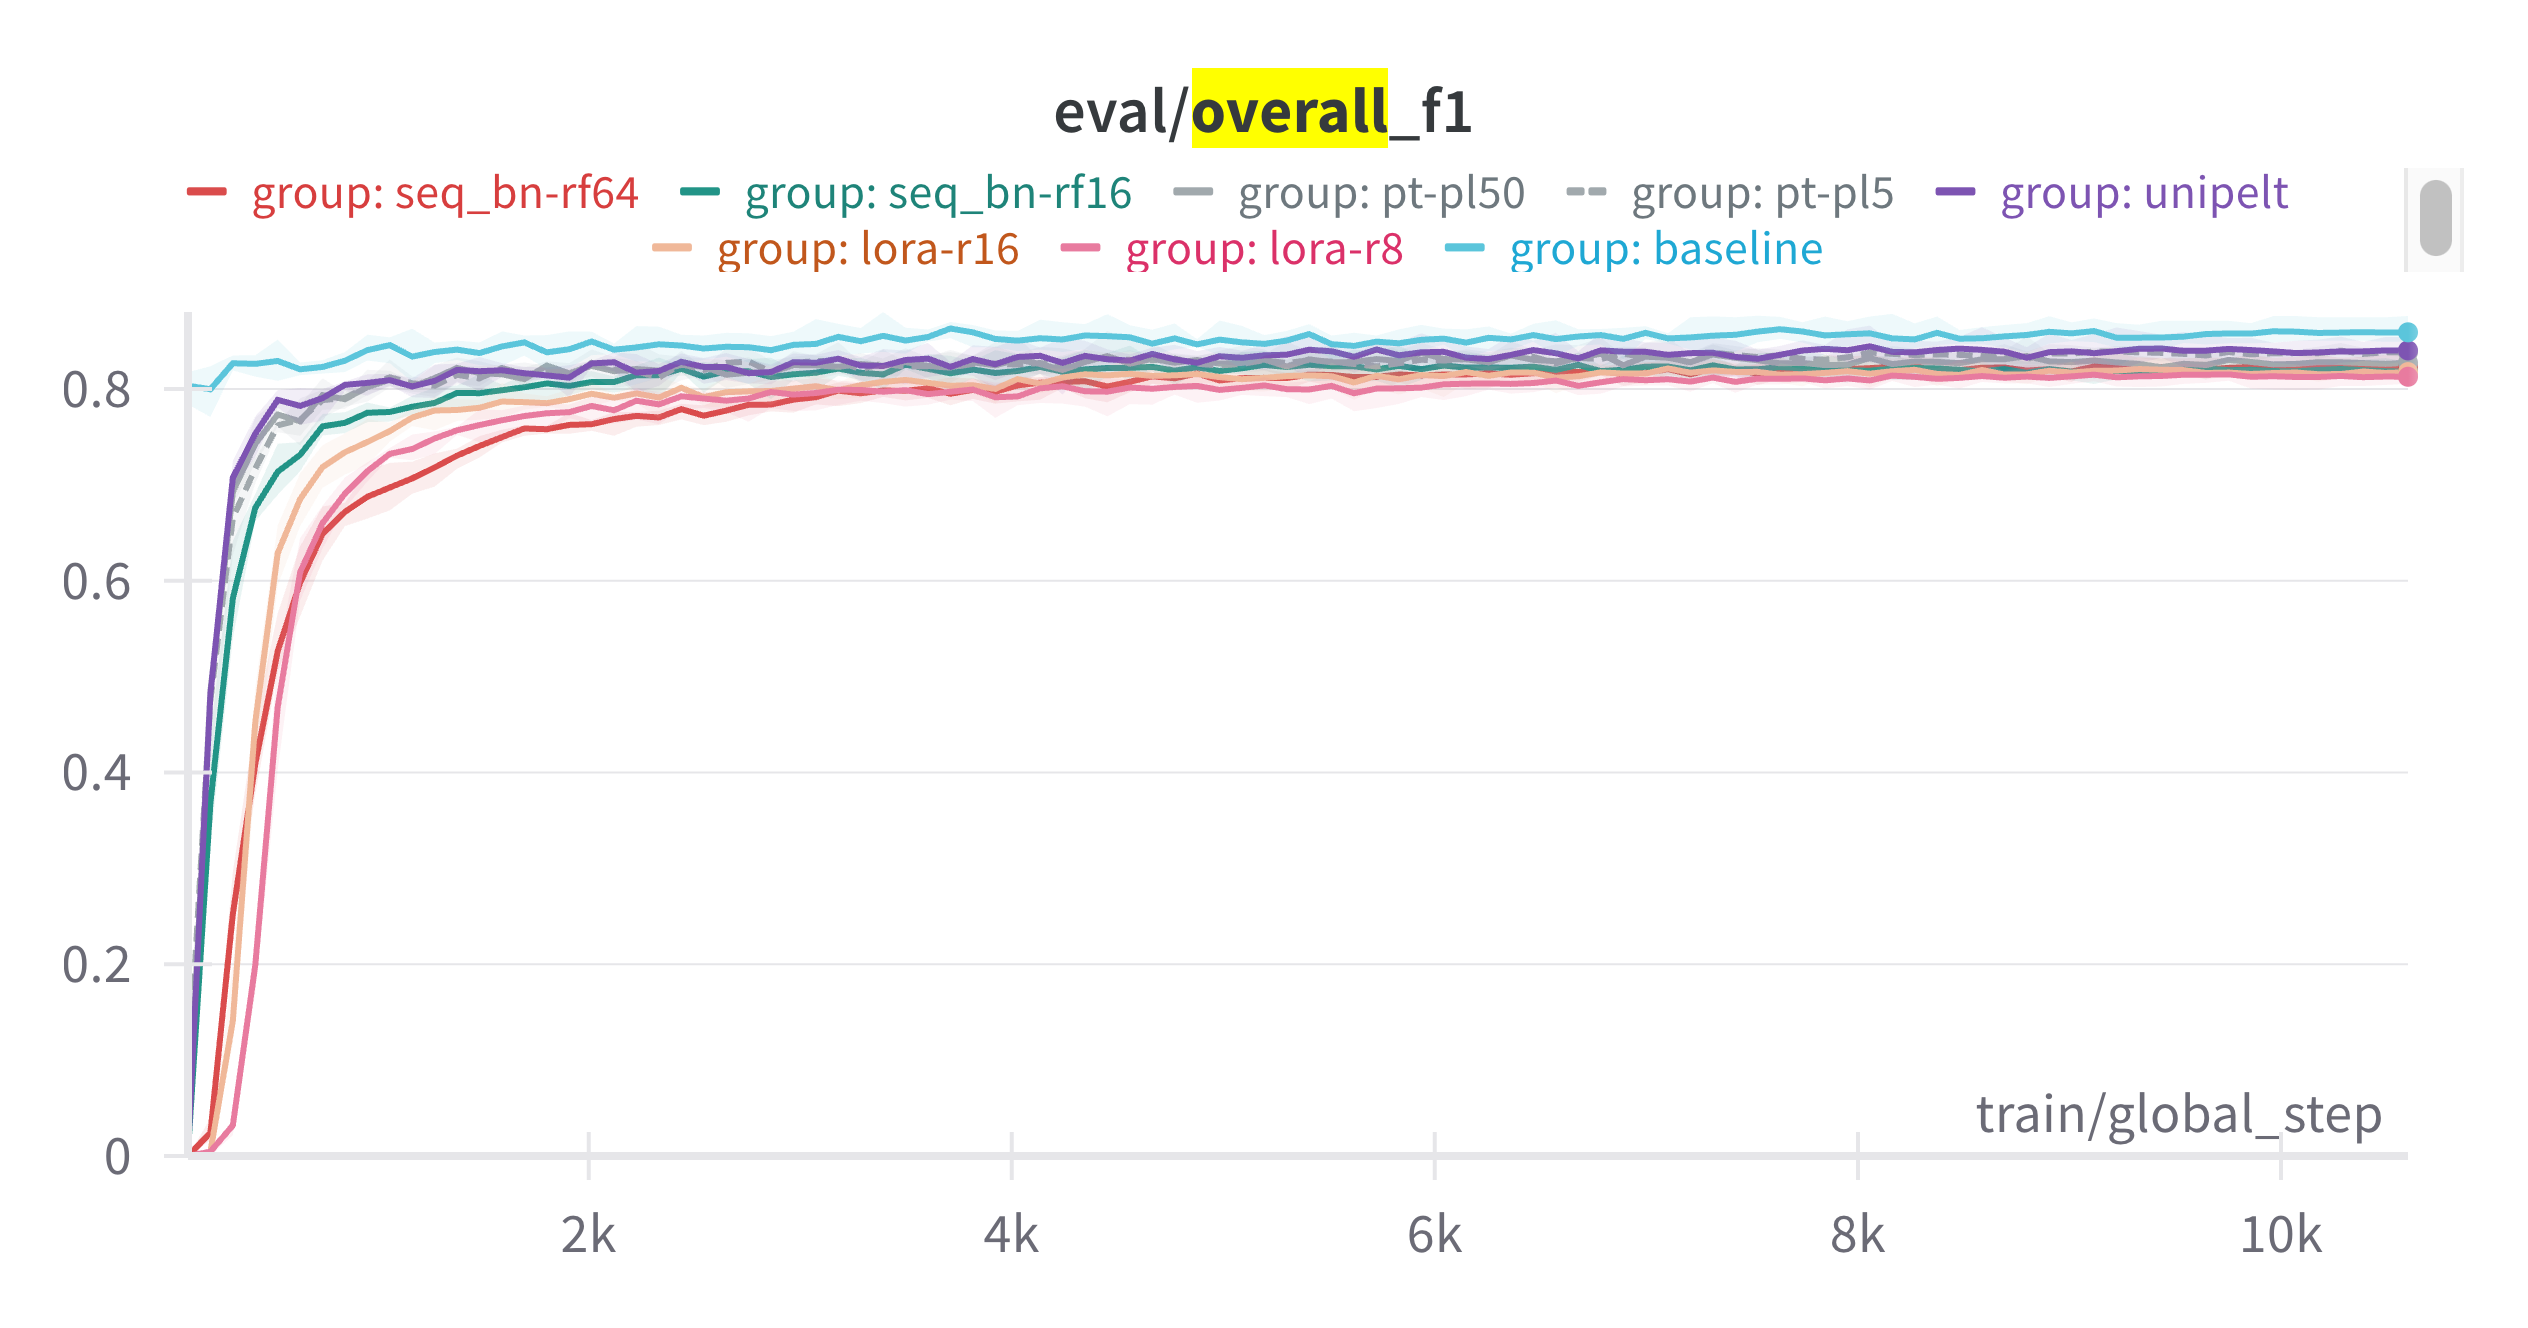
\includegraphics[width=\textwidth]{appendix/nerugm_eval_f1.png} \\
        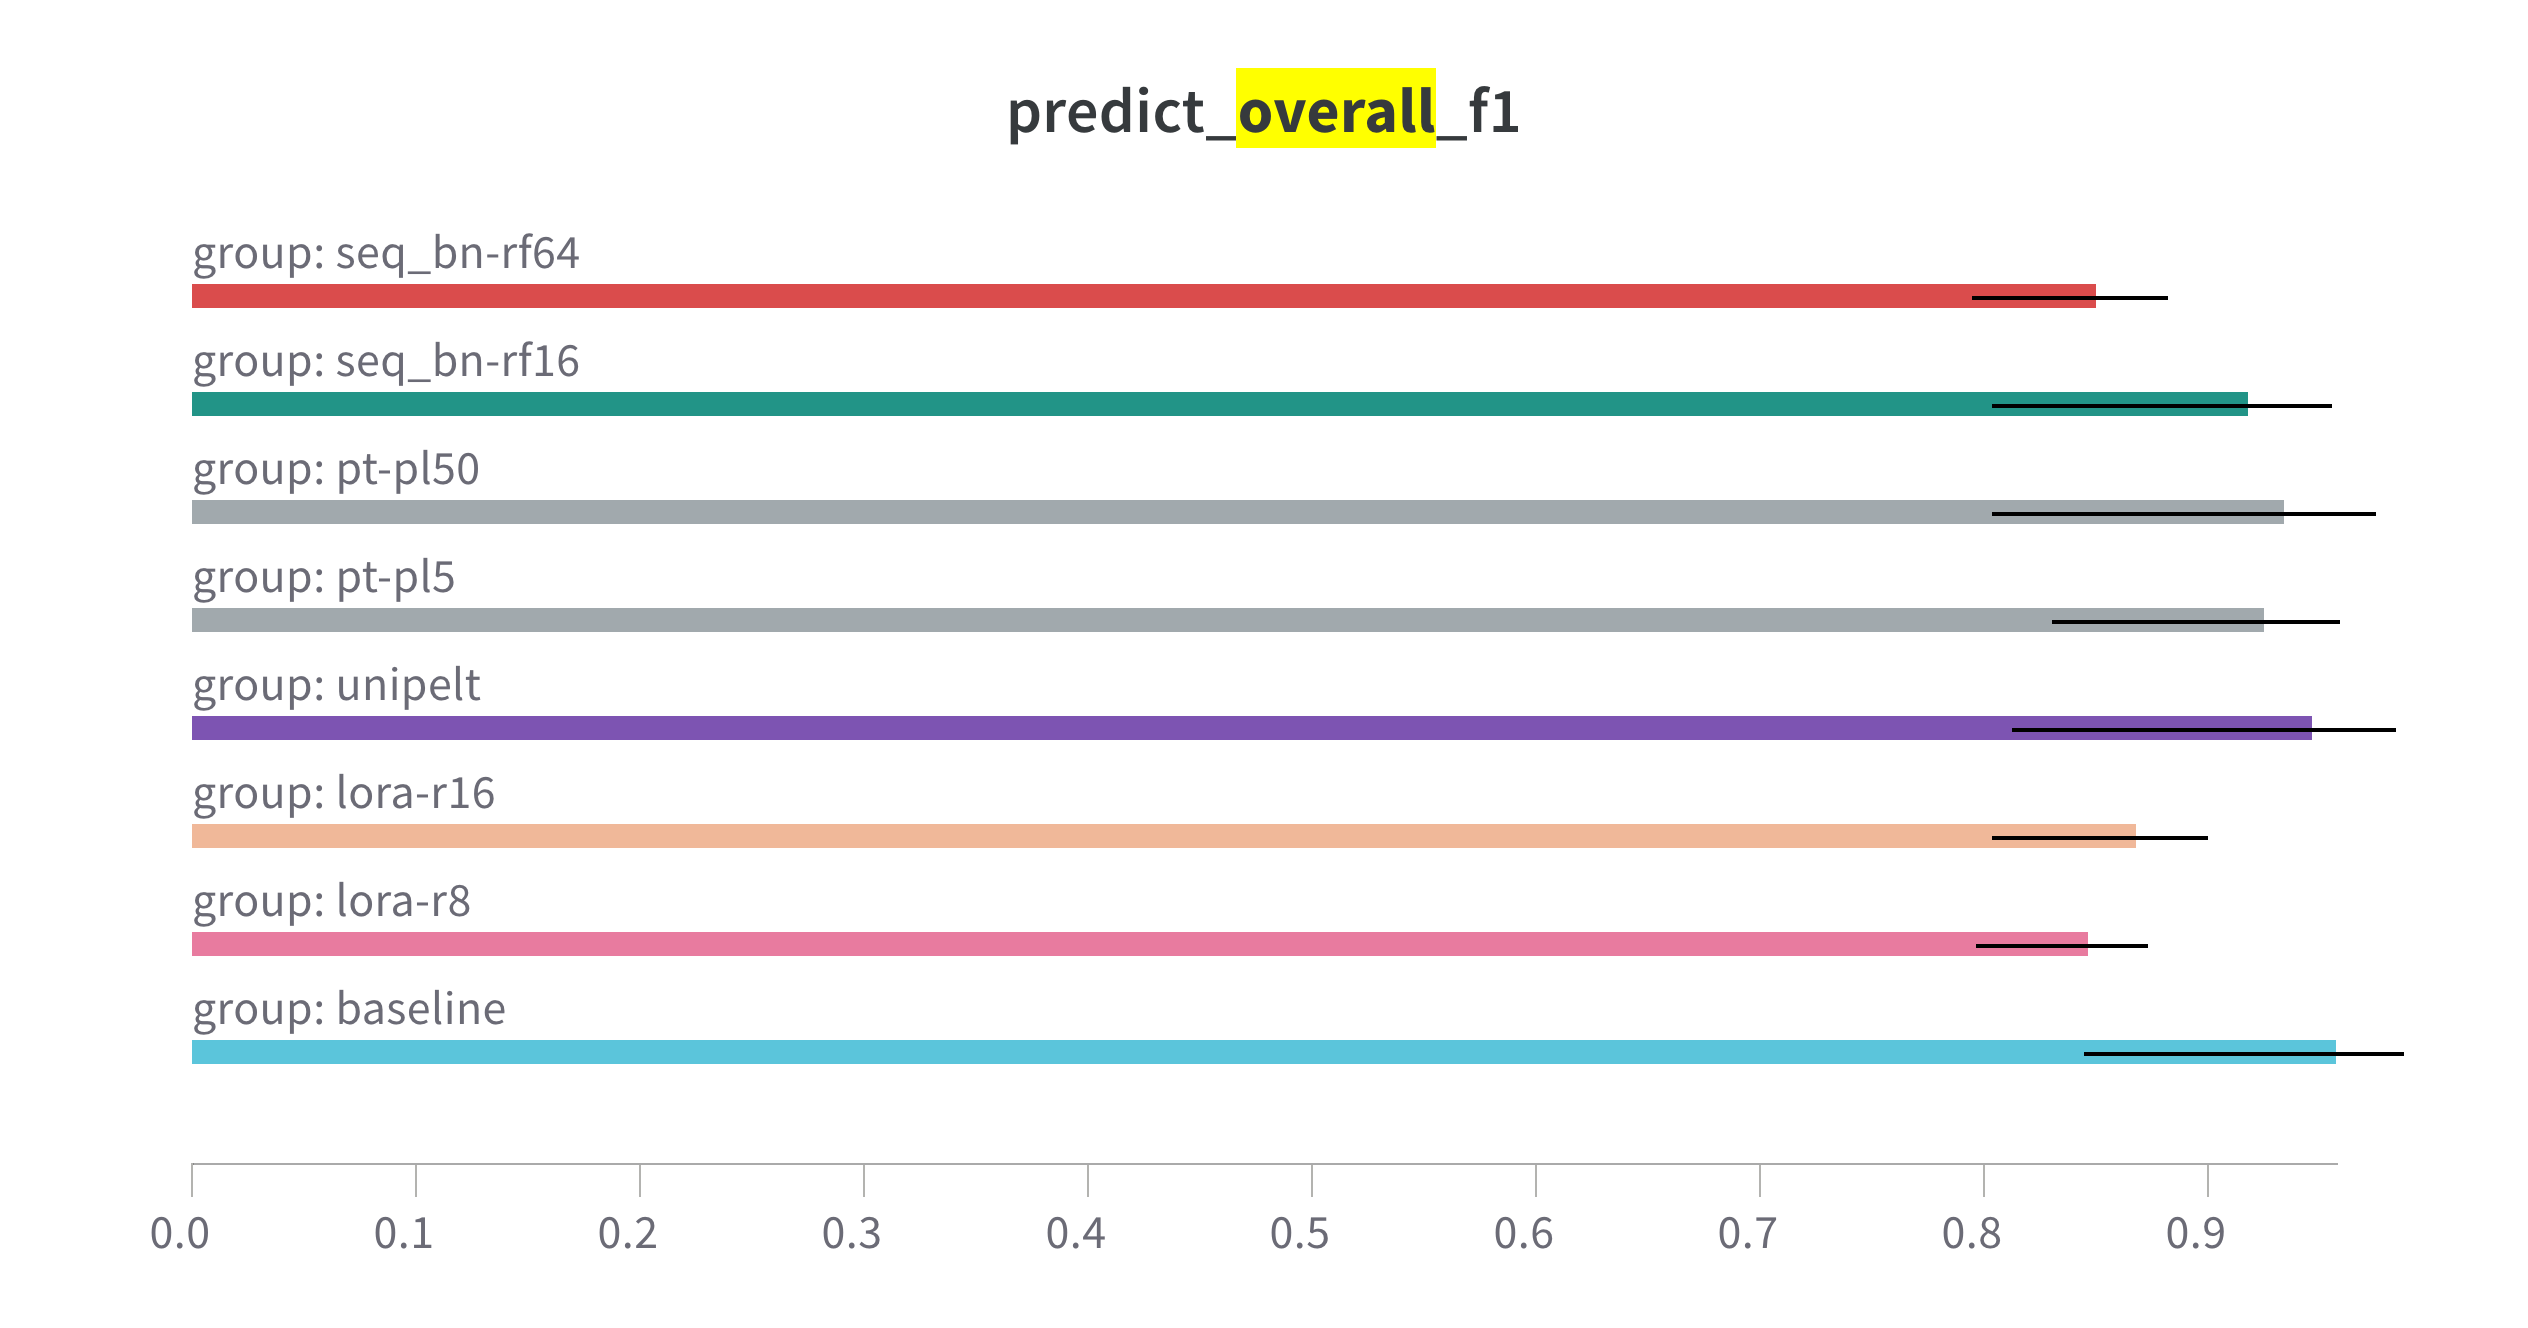
\includegraphics[width=\textwidth]{appendix/nerugm_pred_f1.png} \\
    \end{longtable}
    \caption{Hasil evaluasi dan prediksi F1 tugas NER pada NER UGM}
\end{figure}

\begin{figure}[h]
    \centering
    \begin{longtable}{c}
        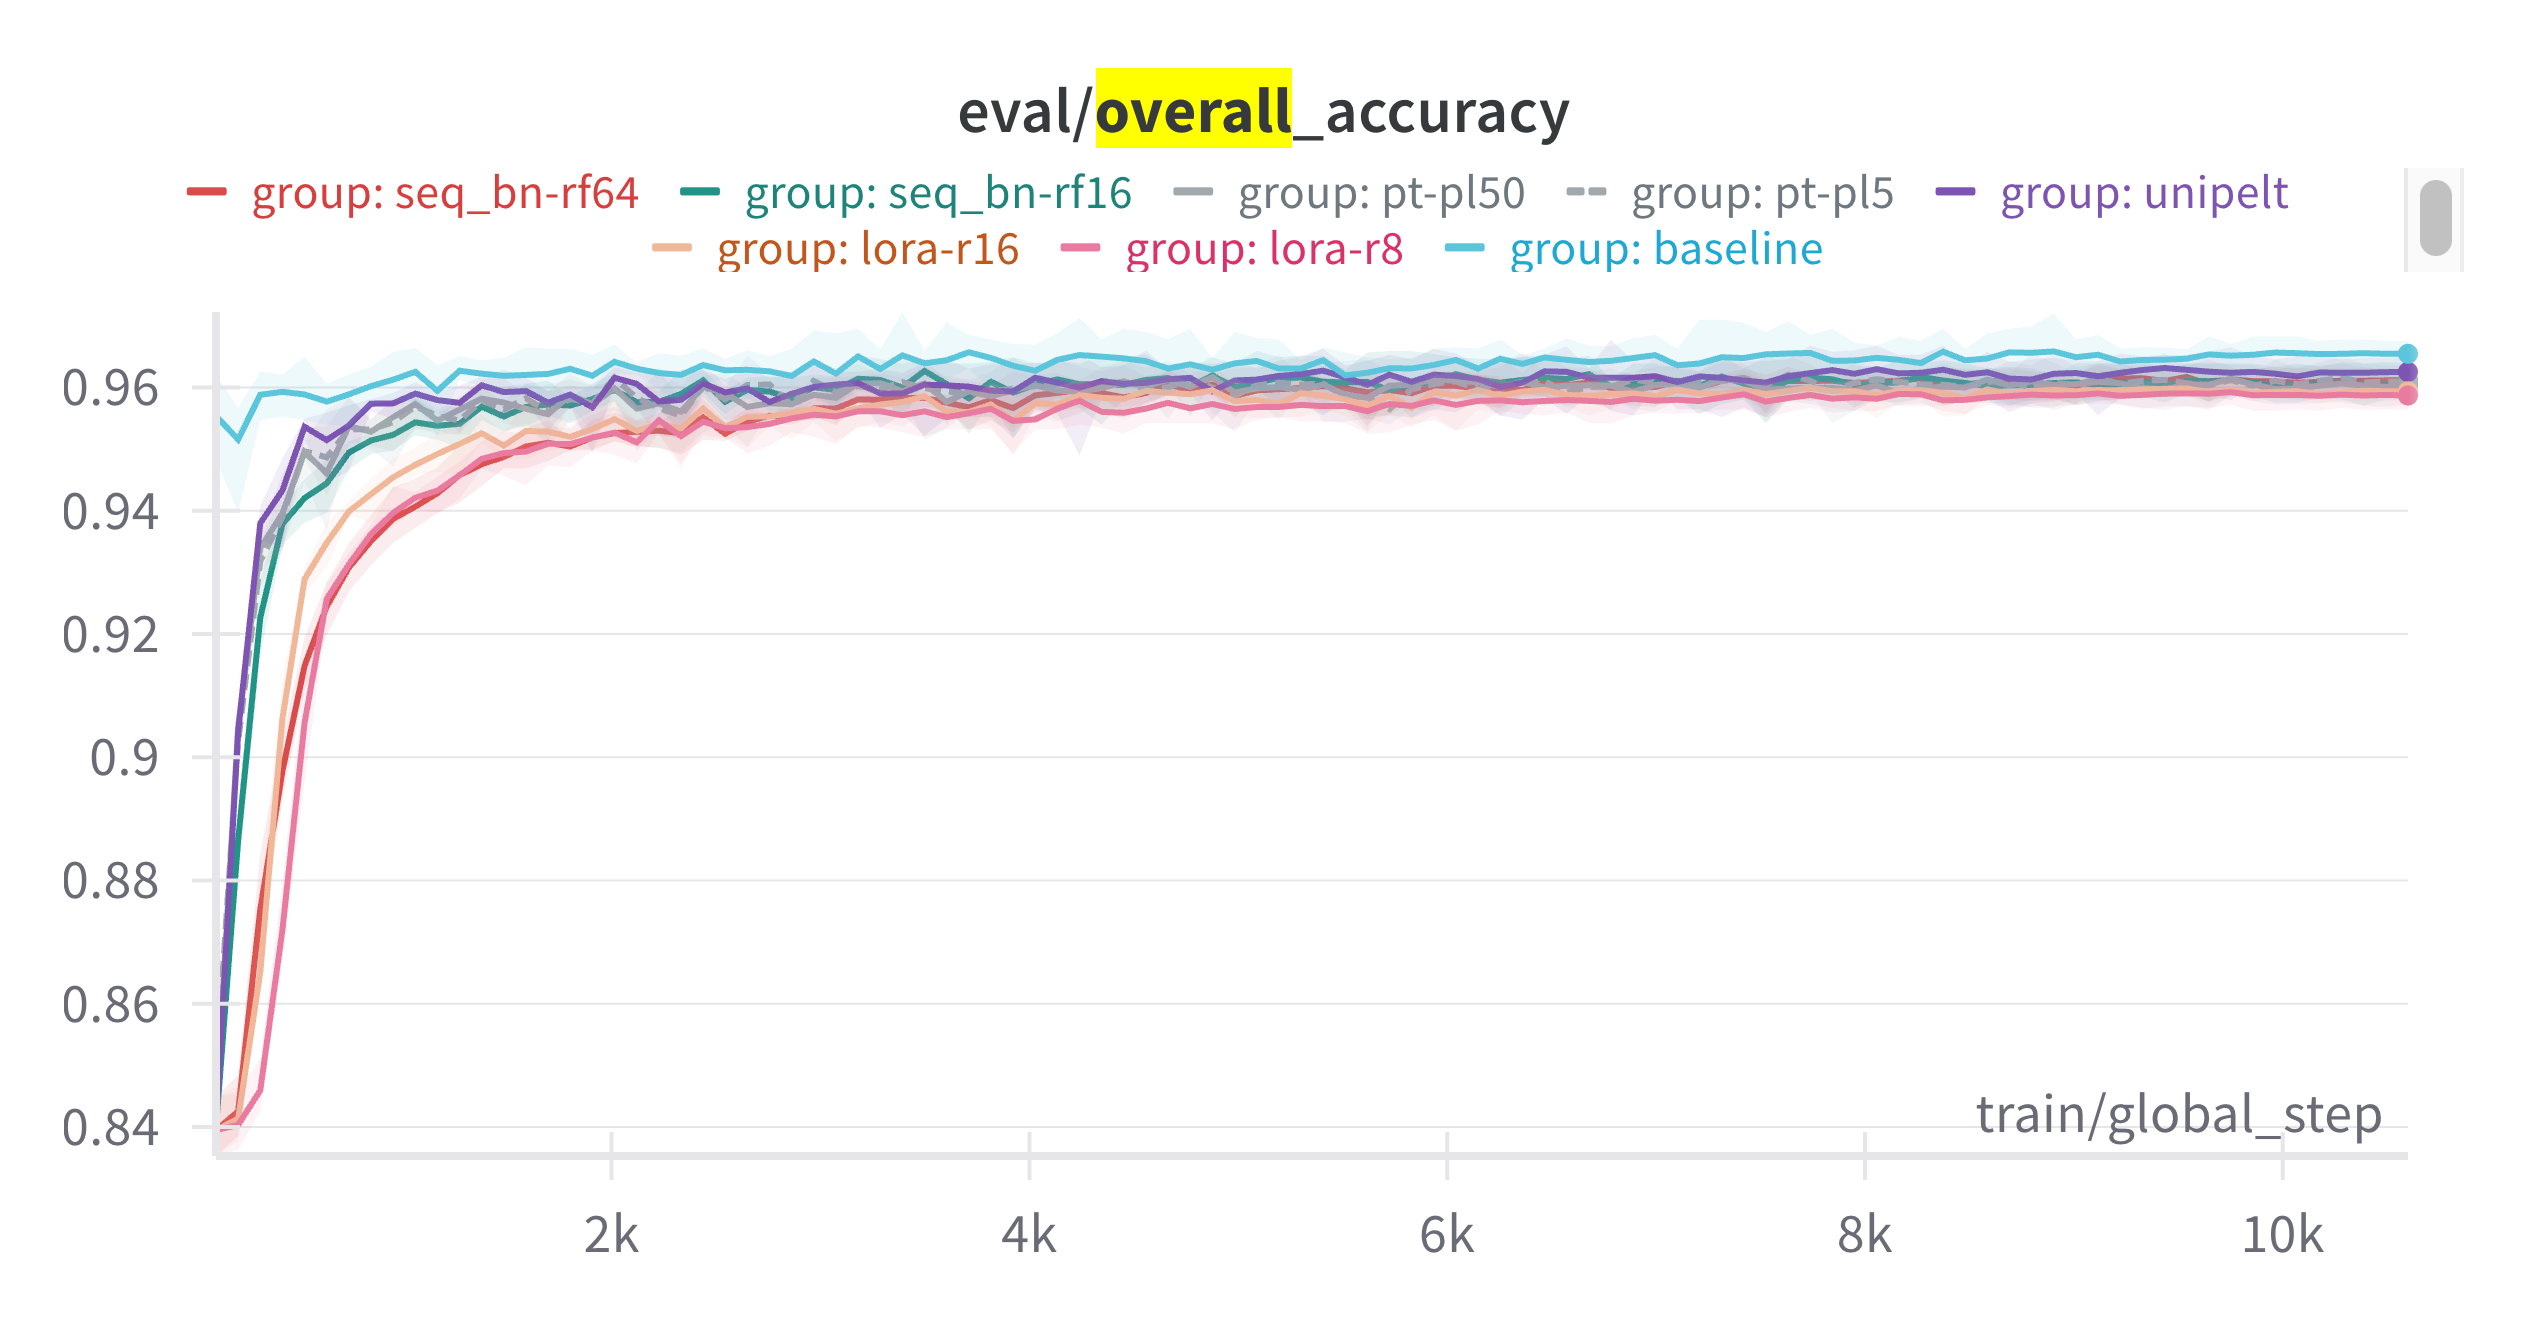
\includegraphics[width=\textwidth]{appendix/nerugm_eval_acc.png} \\
        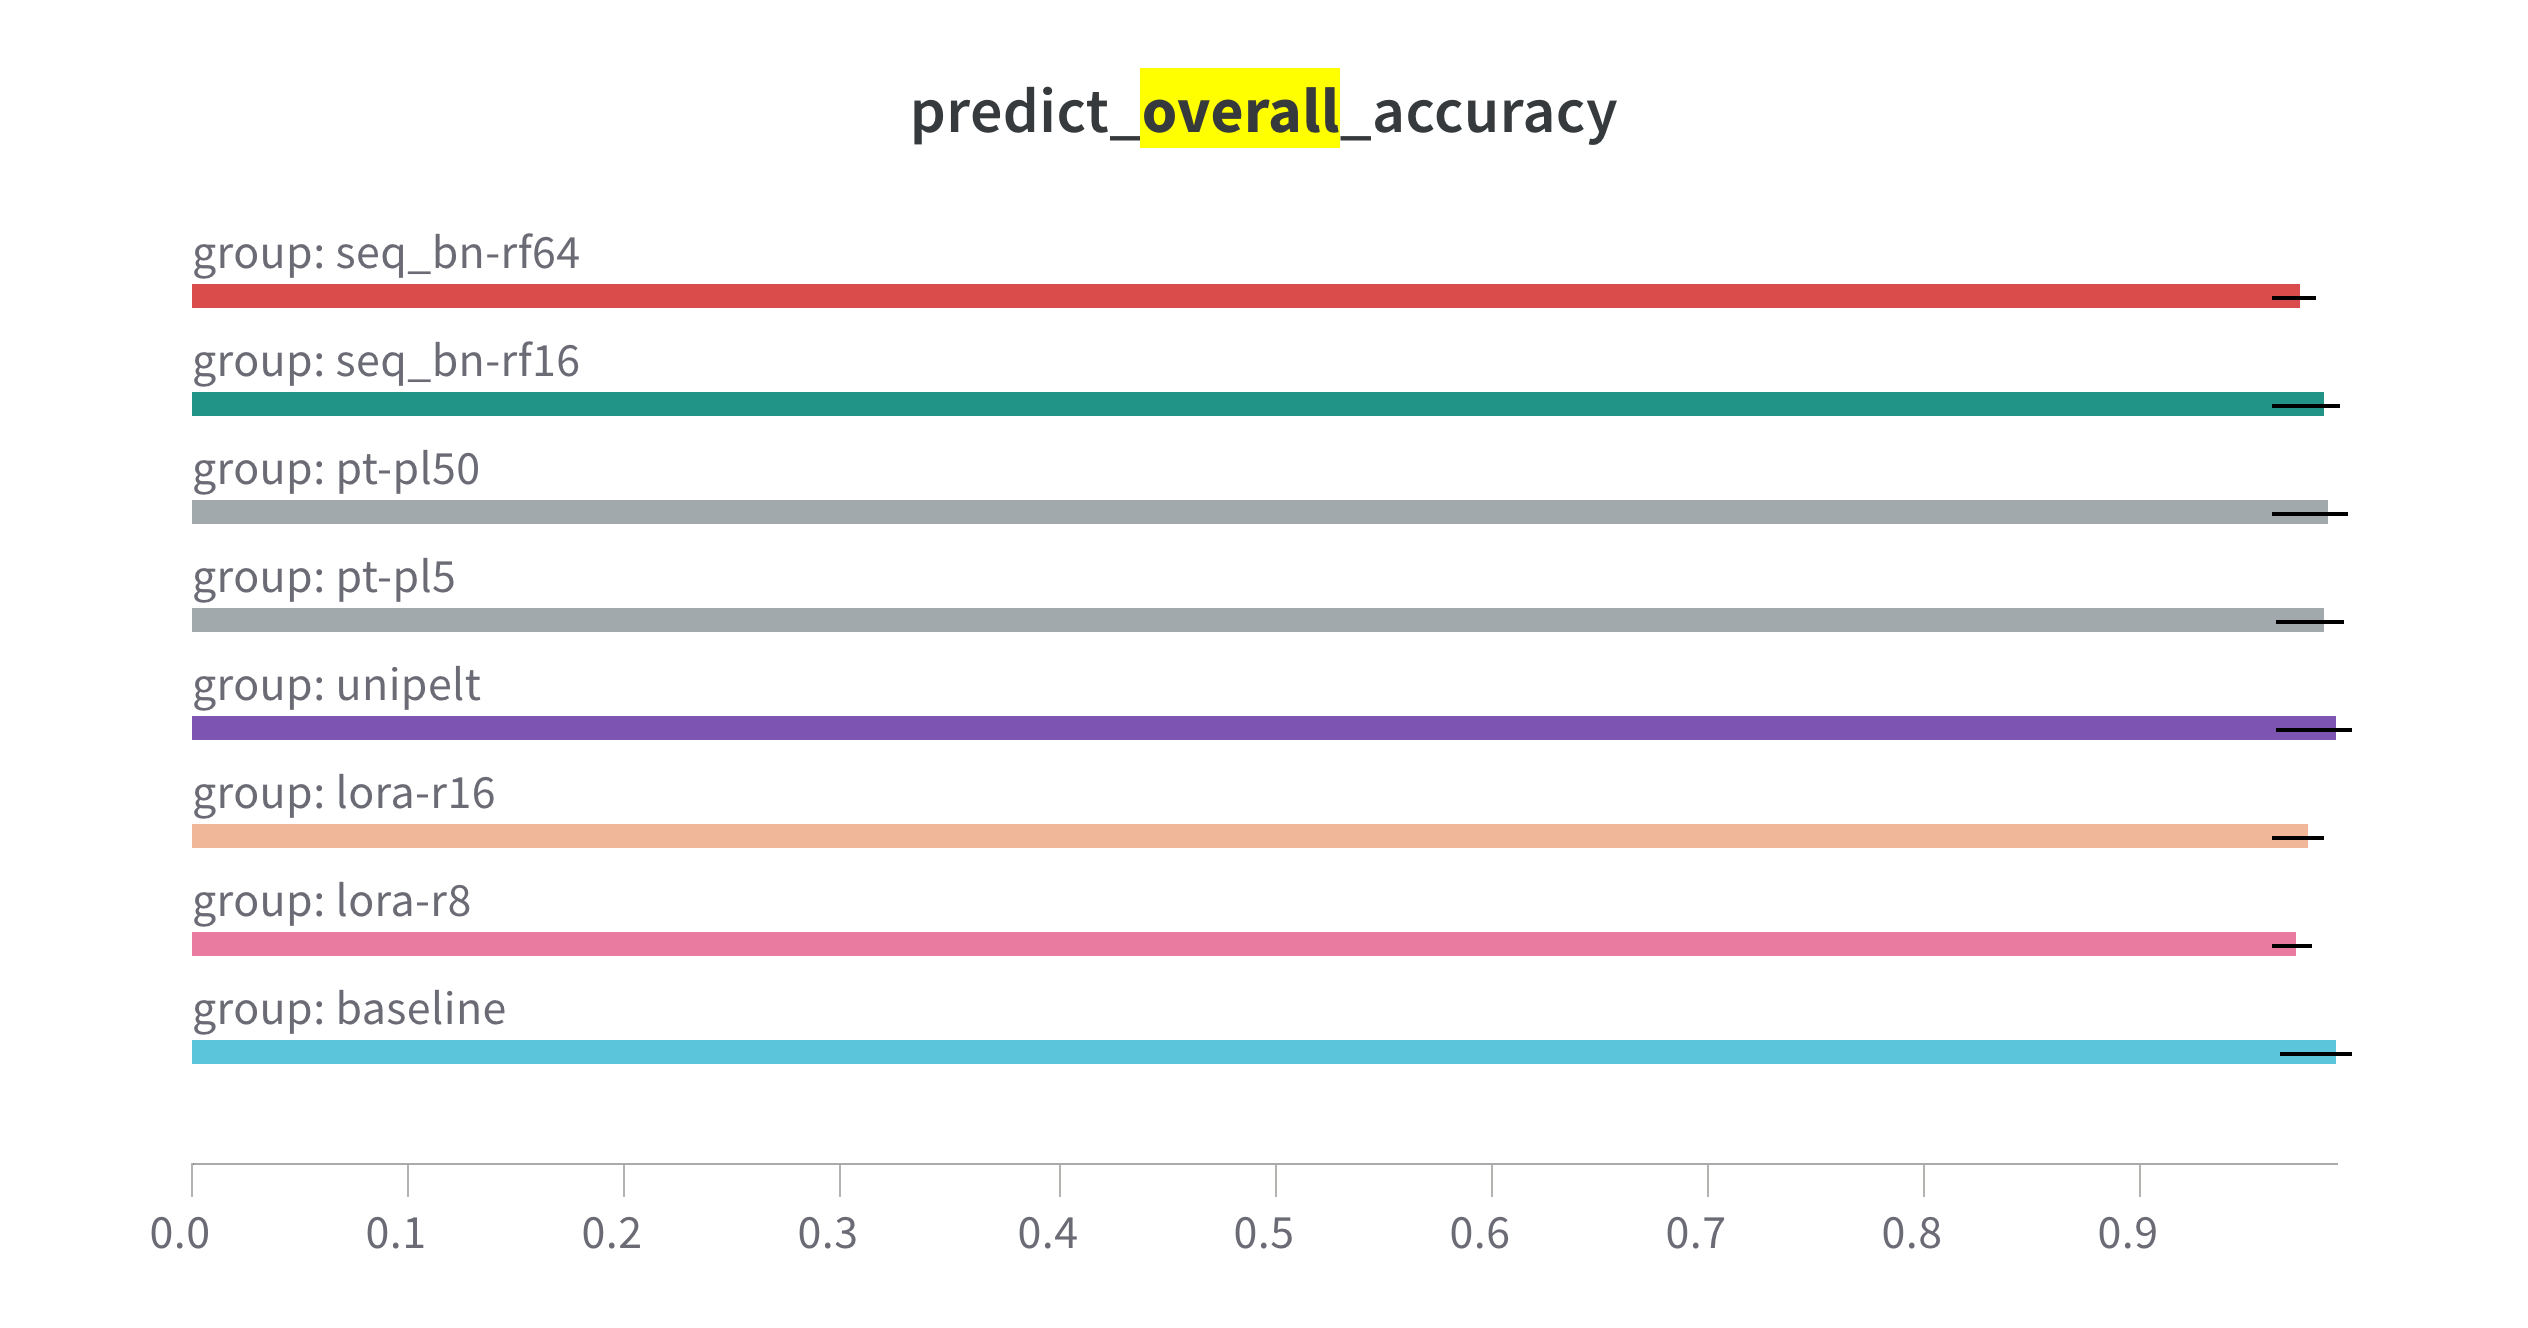
\includegraphics[width=\textwidth]{appendix/nerugm_pred_acc.png} \\
    \end{longtable}
    \caption{Hasil evaluasi dan prediksi \textit{accuracy} tugas NER pada NER UGM}
\end{figure}

\begin{figure}[h]
    \centering
    \begin{longtable}{c}
        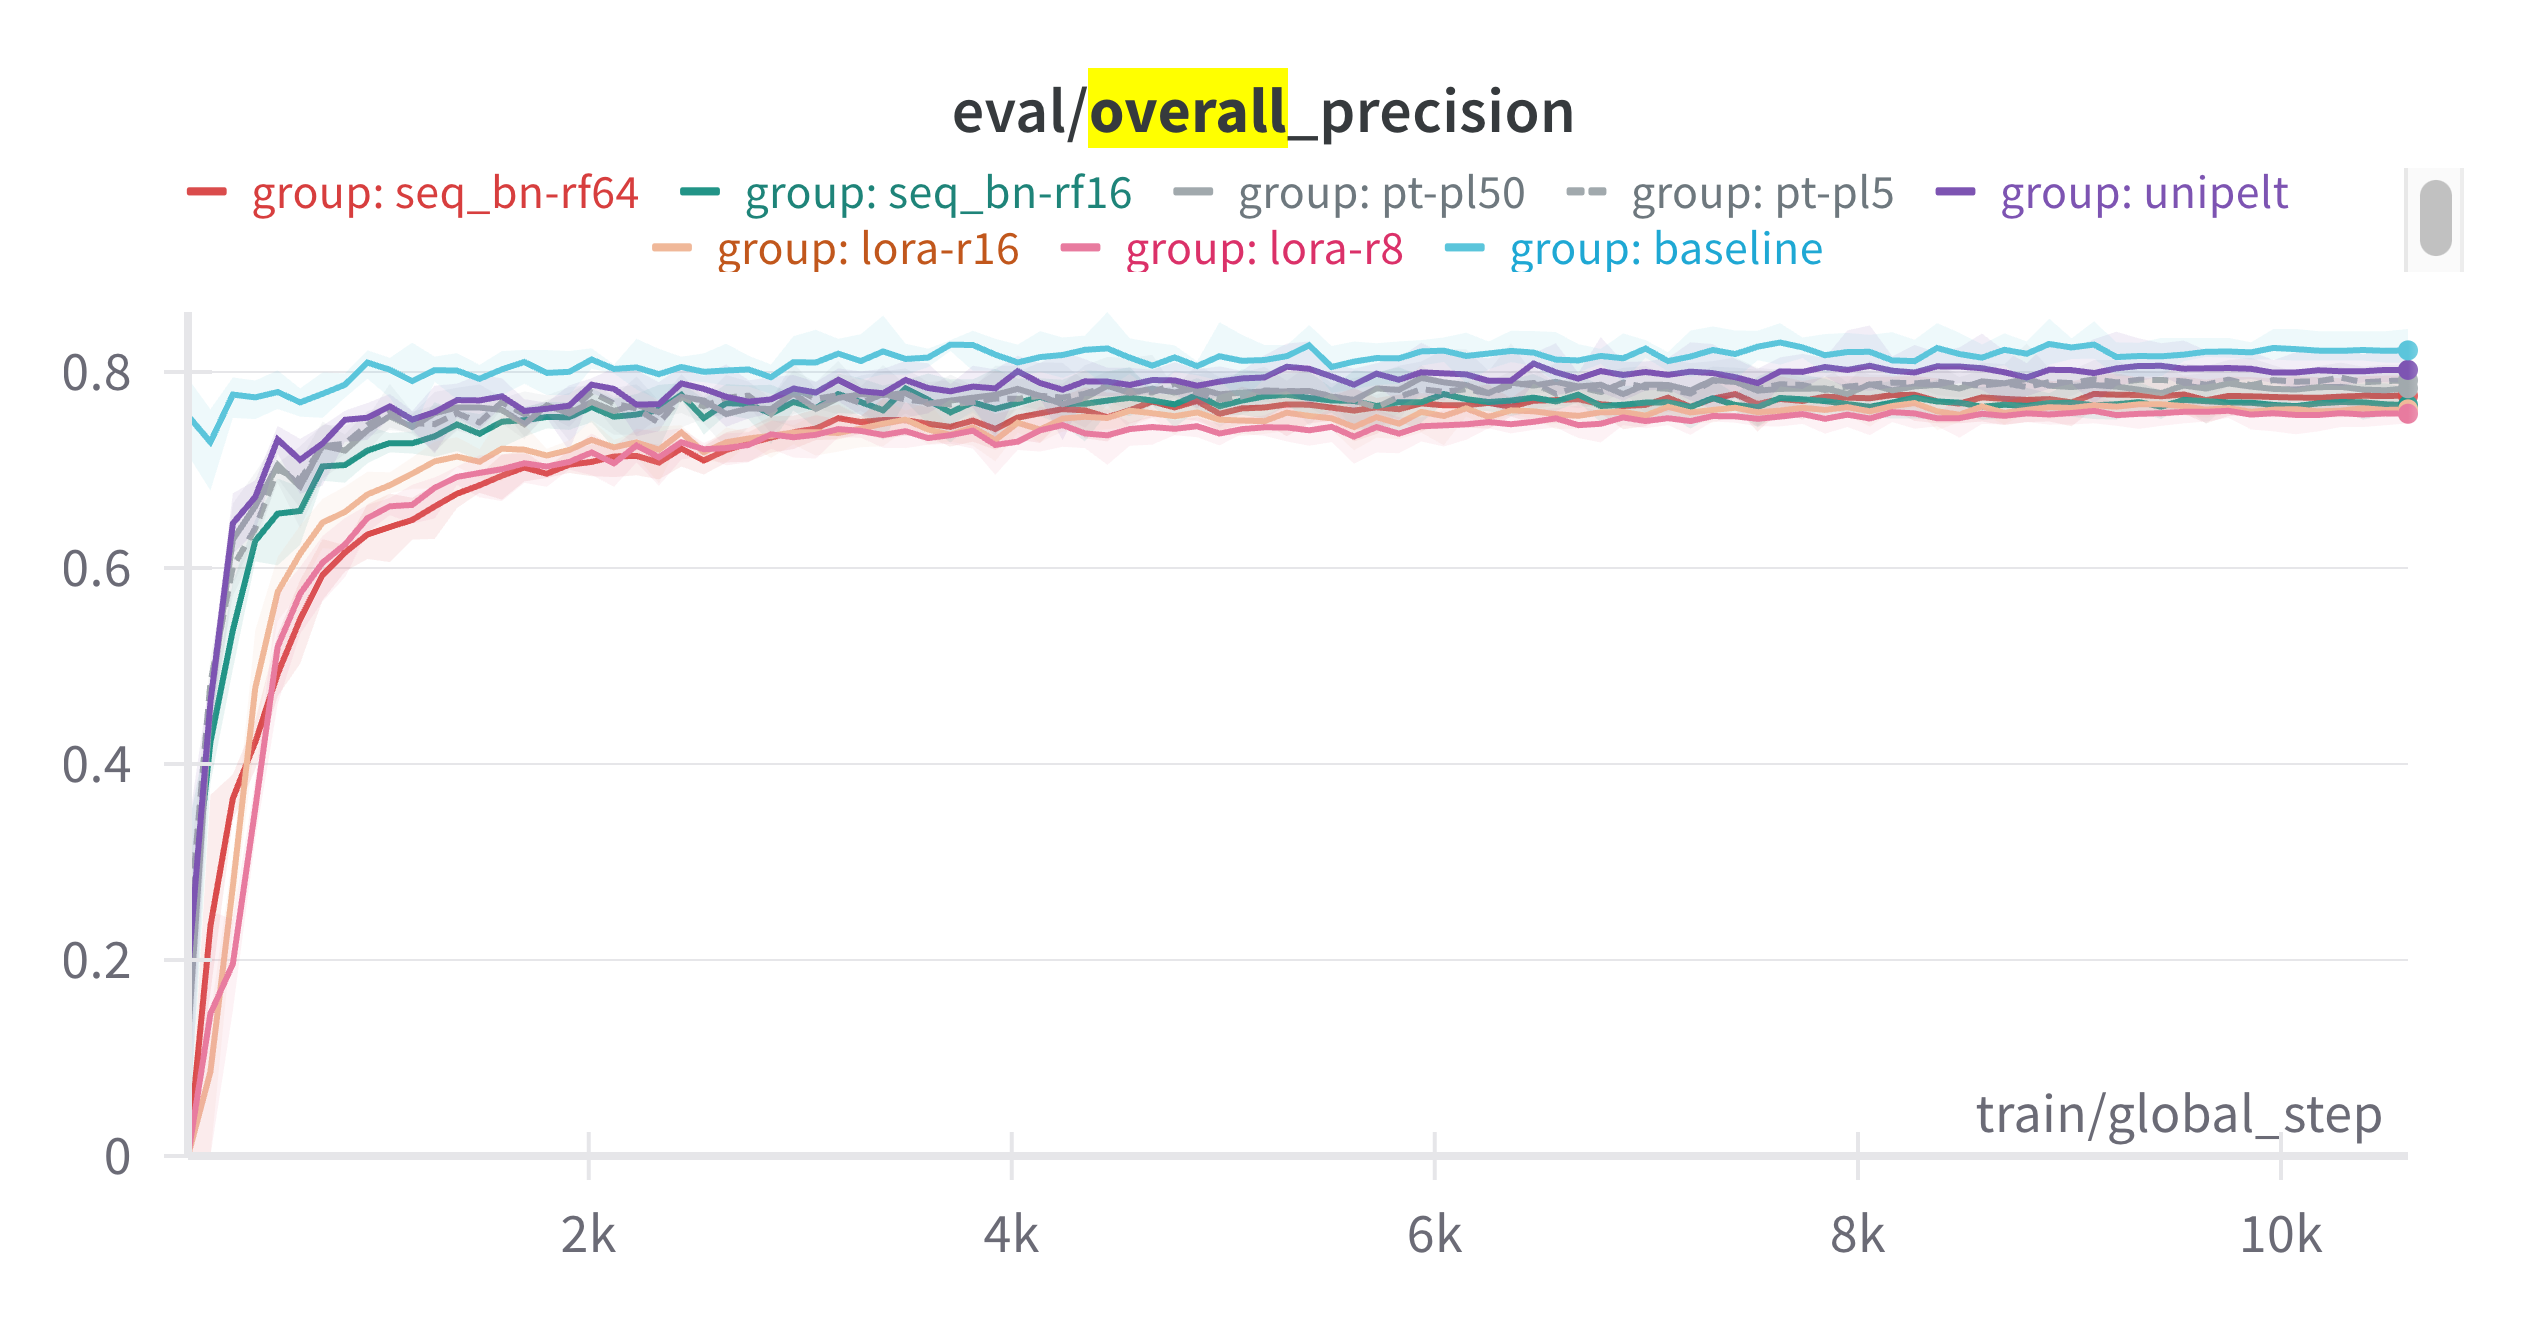
\includegraphics[width=\textwidth]{appendix/nerugm_eval_precision.png} \\
        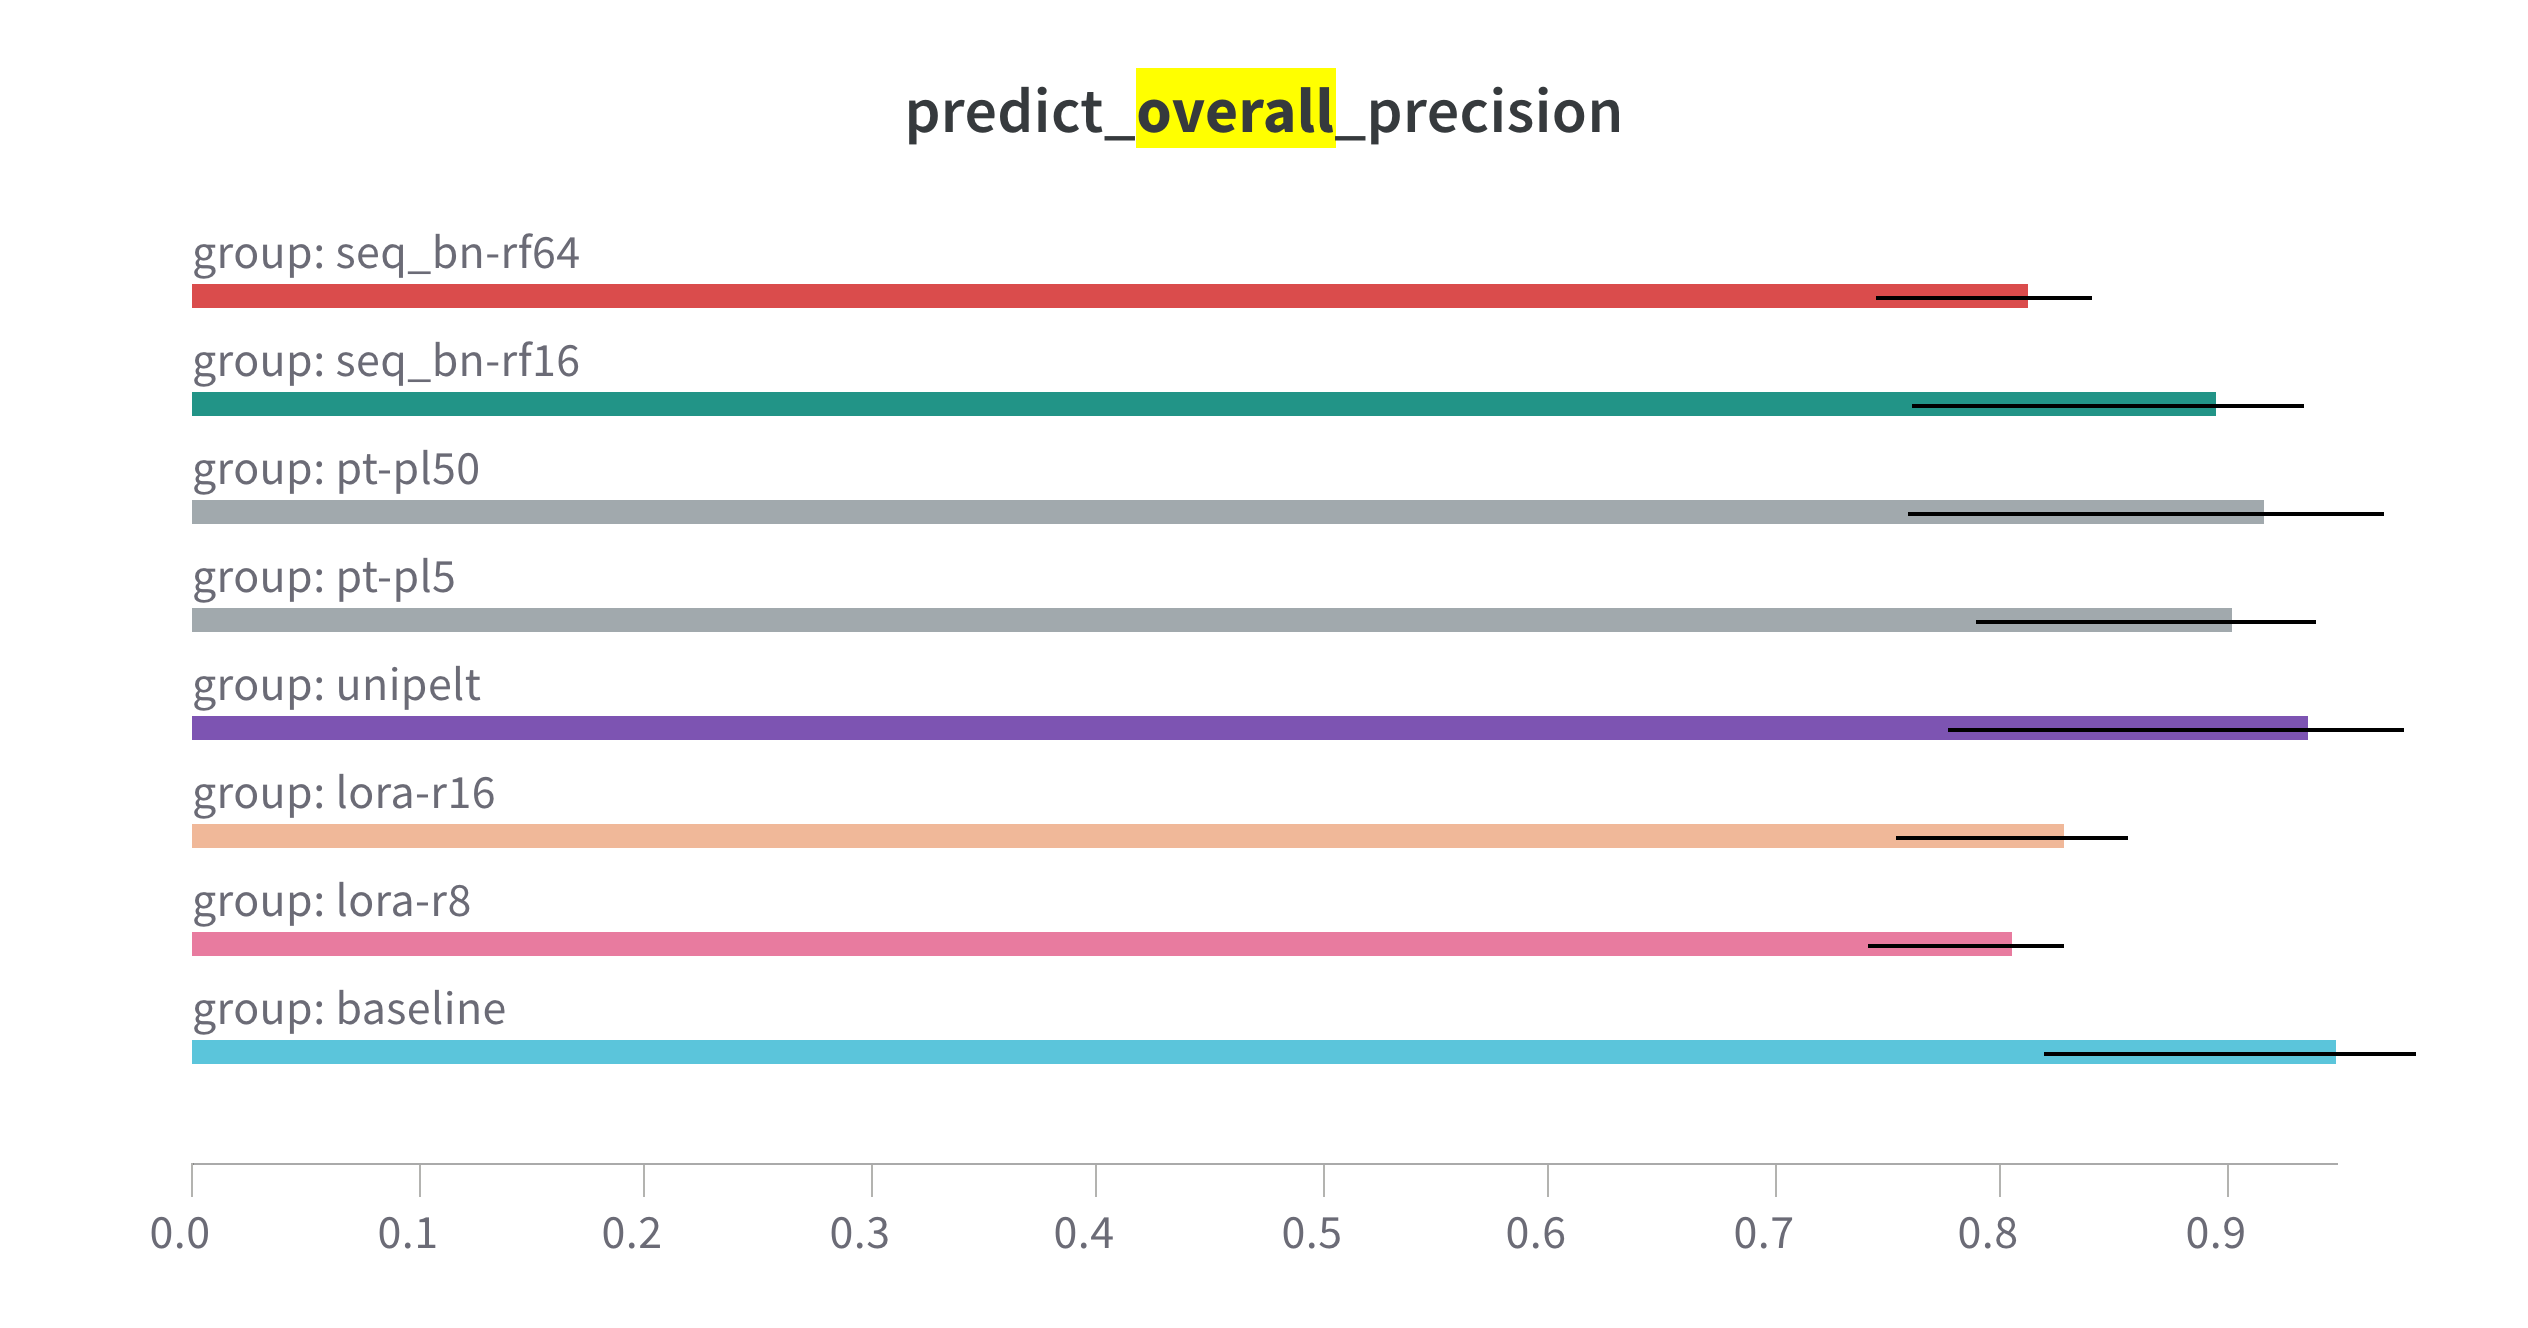
\includegraphics[width=\textwidth]{appendix/nerugm_pred_precision.png} \\
    \end{longtable}
    \caption{Hasil evaluasi dan prediksi \textit{precision} tugas NER pada NER UGM}
\end{figure}

\begin{figure}[h]
    \centering
    \begin{longtable}{c}
        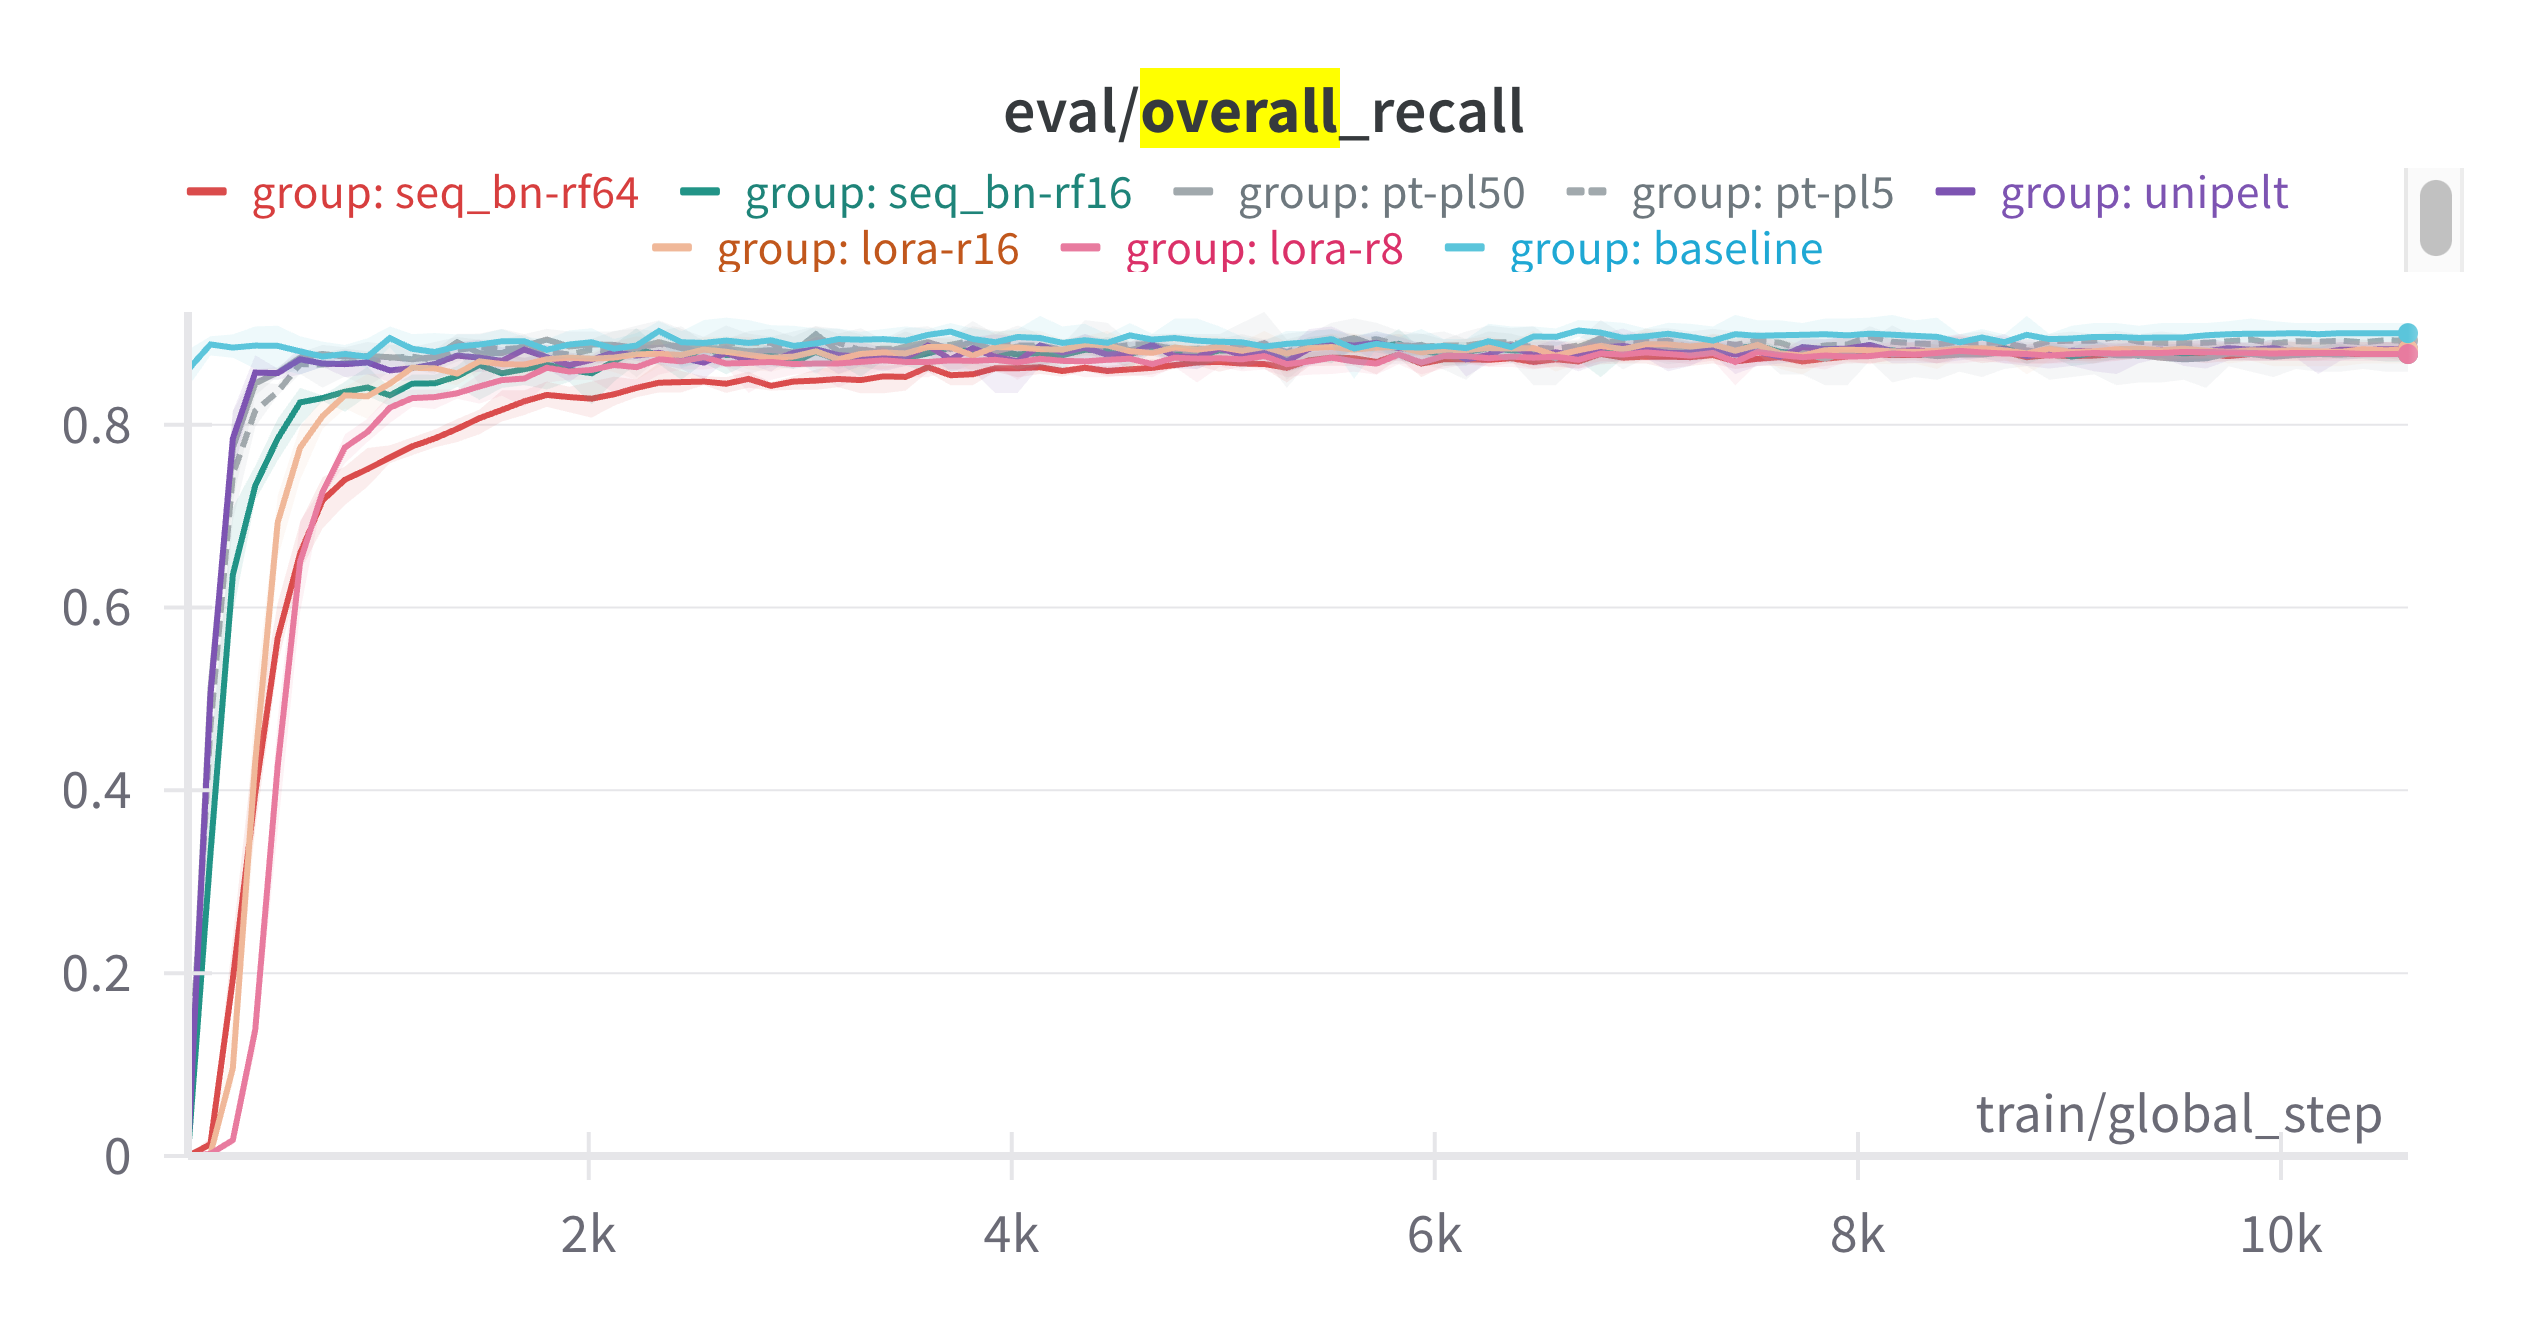
\includegraphics[width=\textwidth]{appendix/nerugm_eval_recall.png} \\
        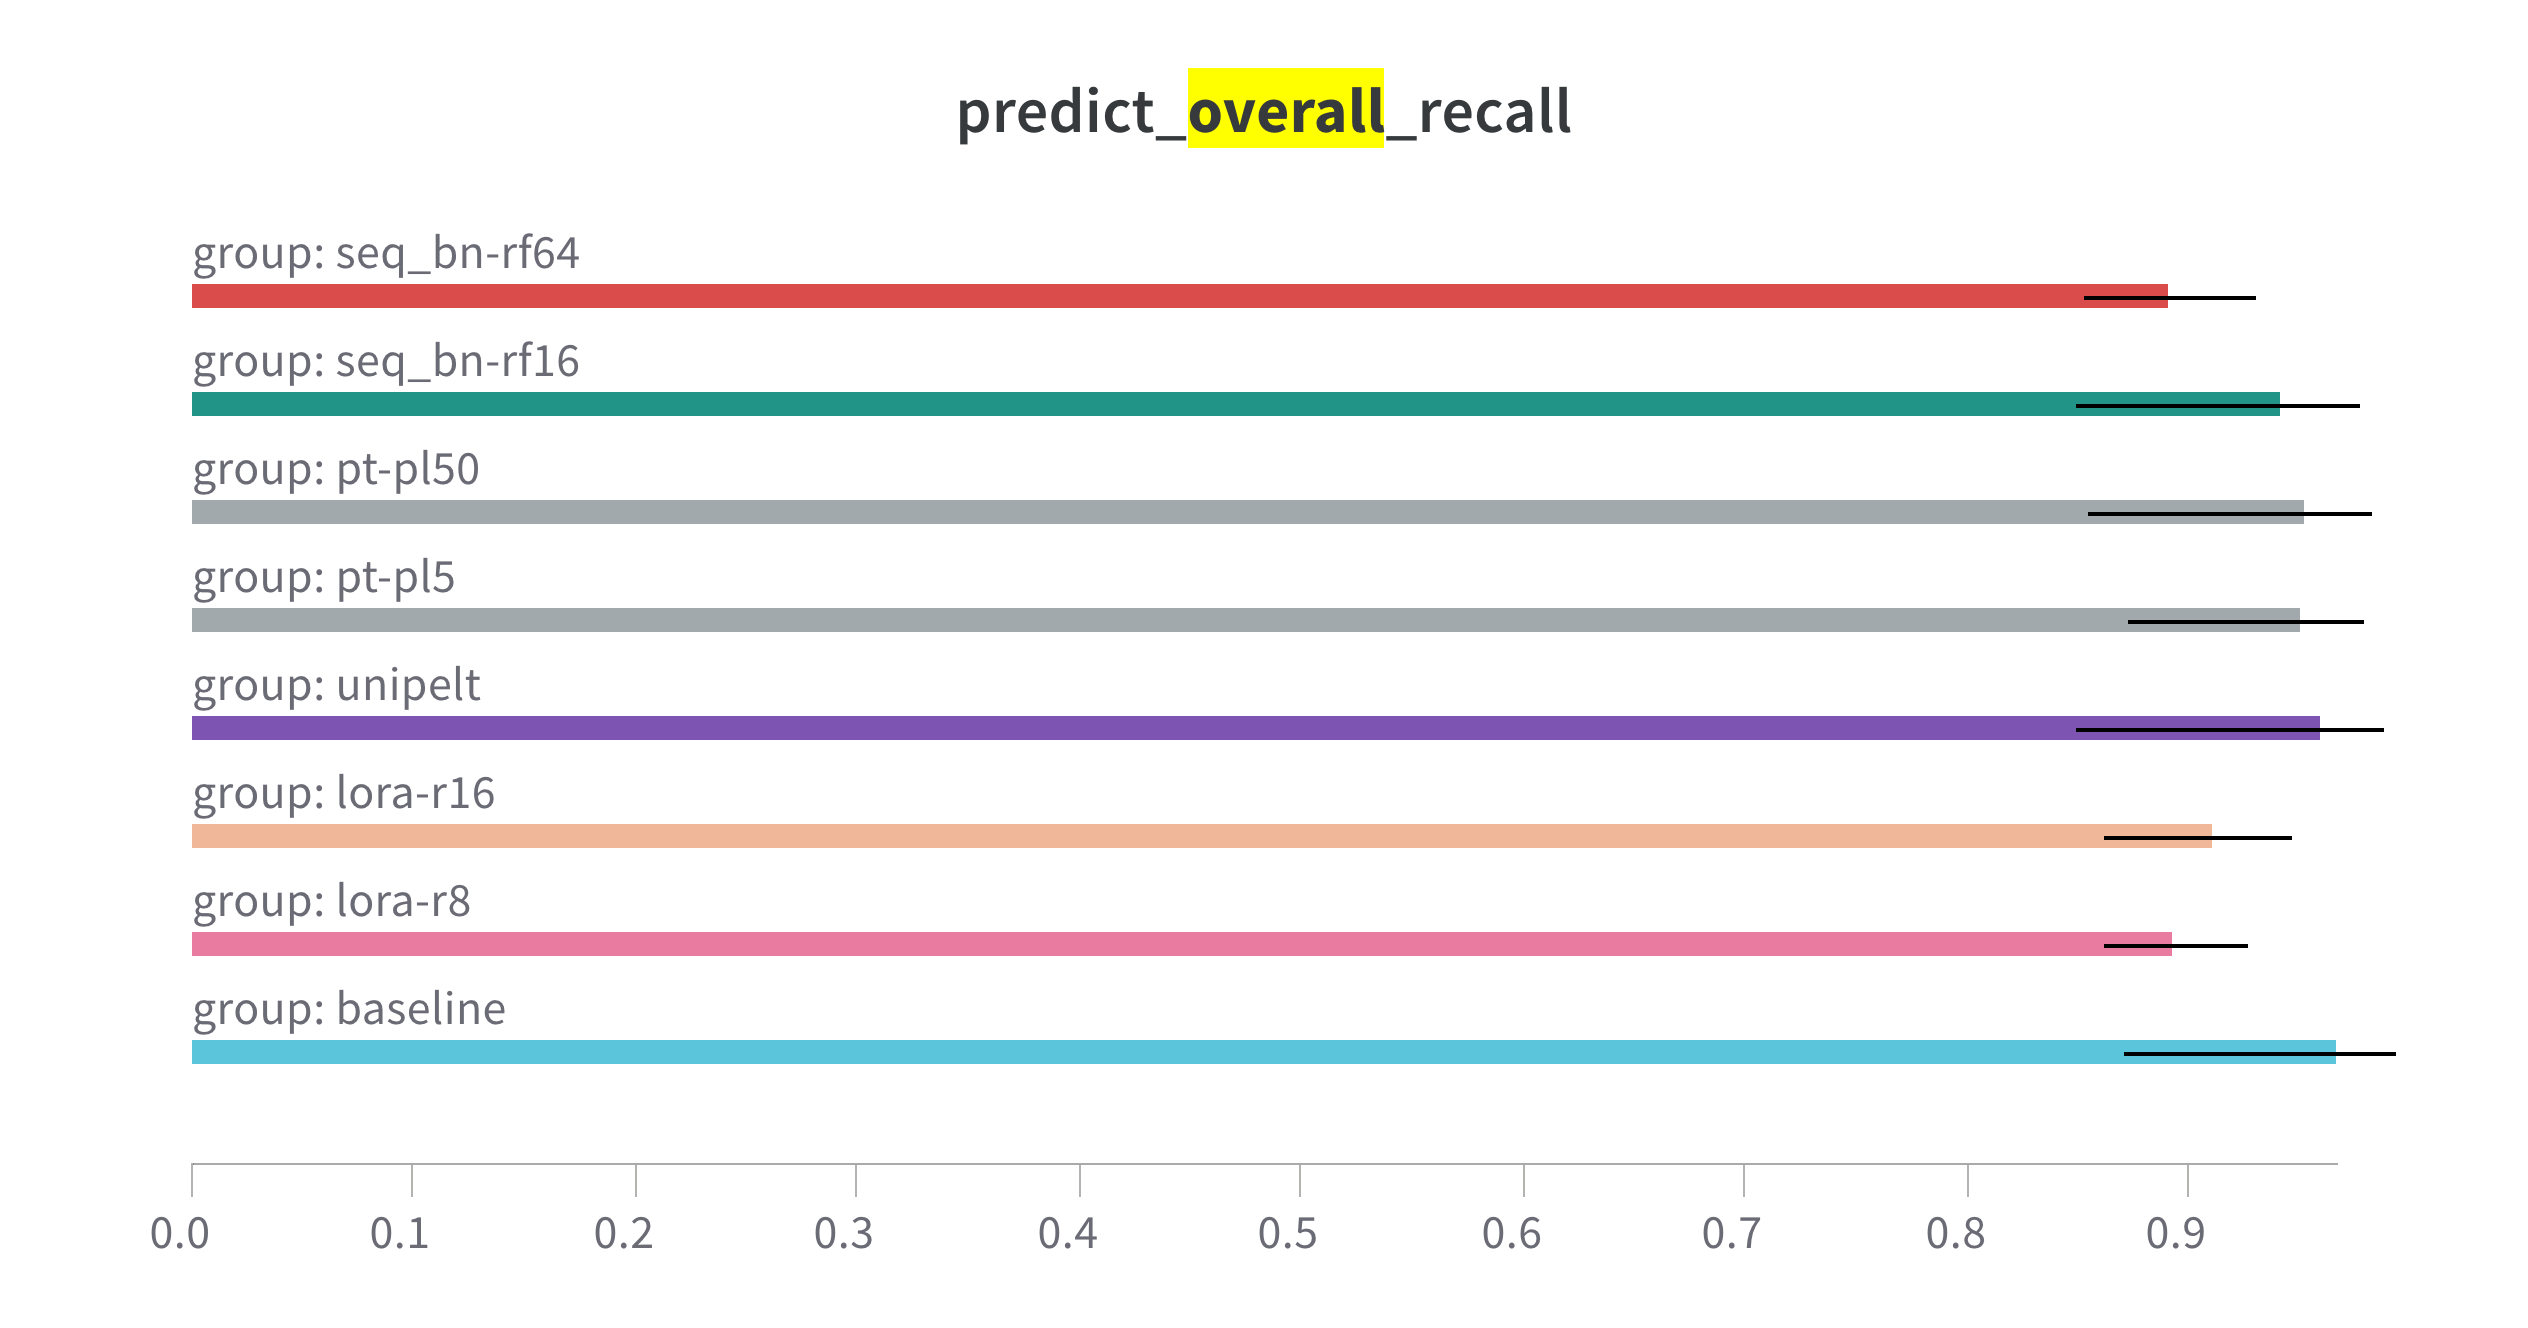
\includegraphics[width=\textwidth]{appendix/nerugm_pred_recall.png} \\
    \end{longtable}
    \caption{Hasil evaluasi dan prediksi \textit{recall} tugas NER pada NER UGM}
\end{figure}

\chapter{Hasil Evaluasi dan Prediksi Tugas \textit{Sentiment Analysis}}
\label{appendix:sentiment}

\begin{figure}[h]
    \centering
    \begin{longtable}{c}
        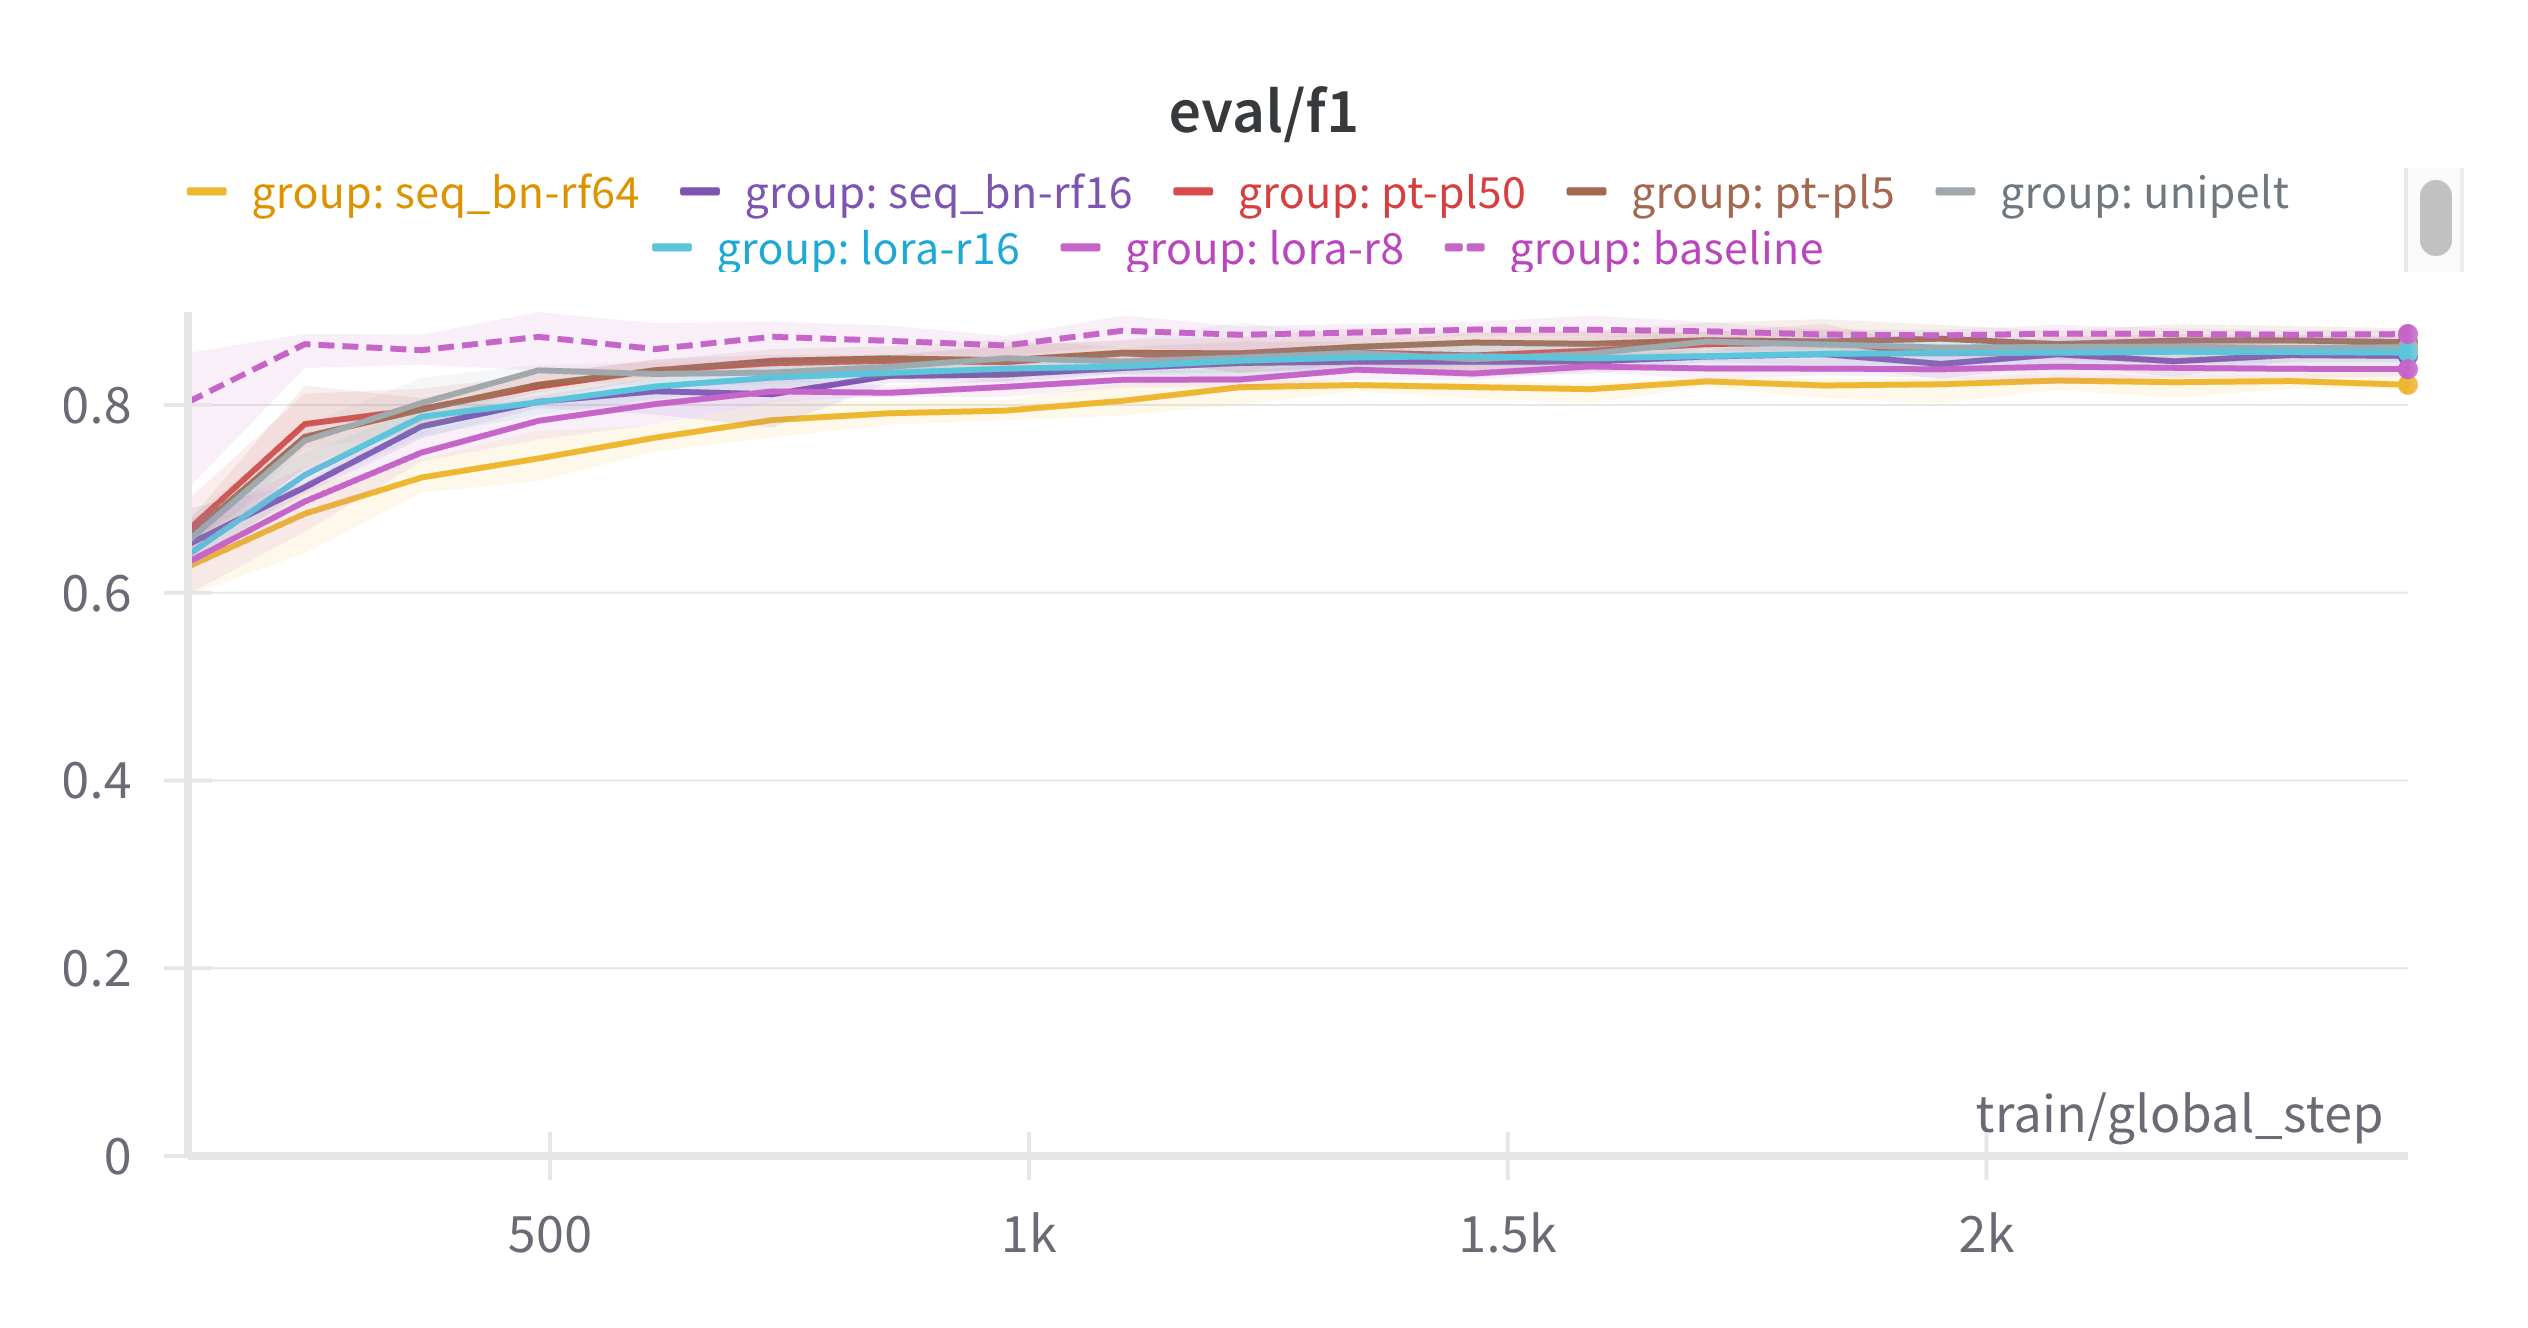
\includegraphics[width=\textwidth]{appendix/sentiment_eval_f1.png} \\
        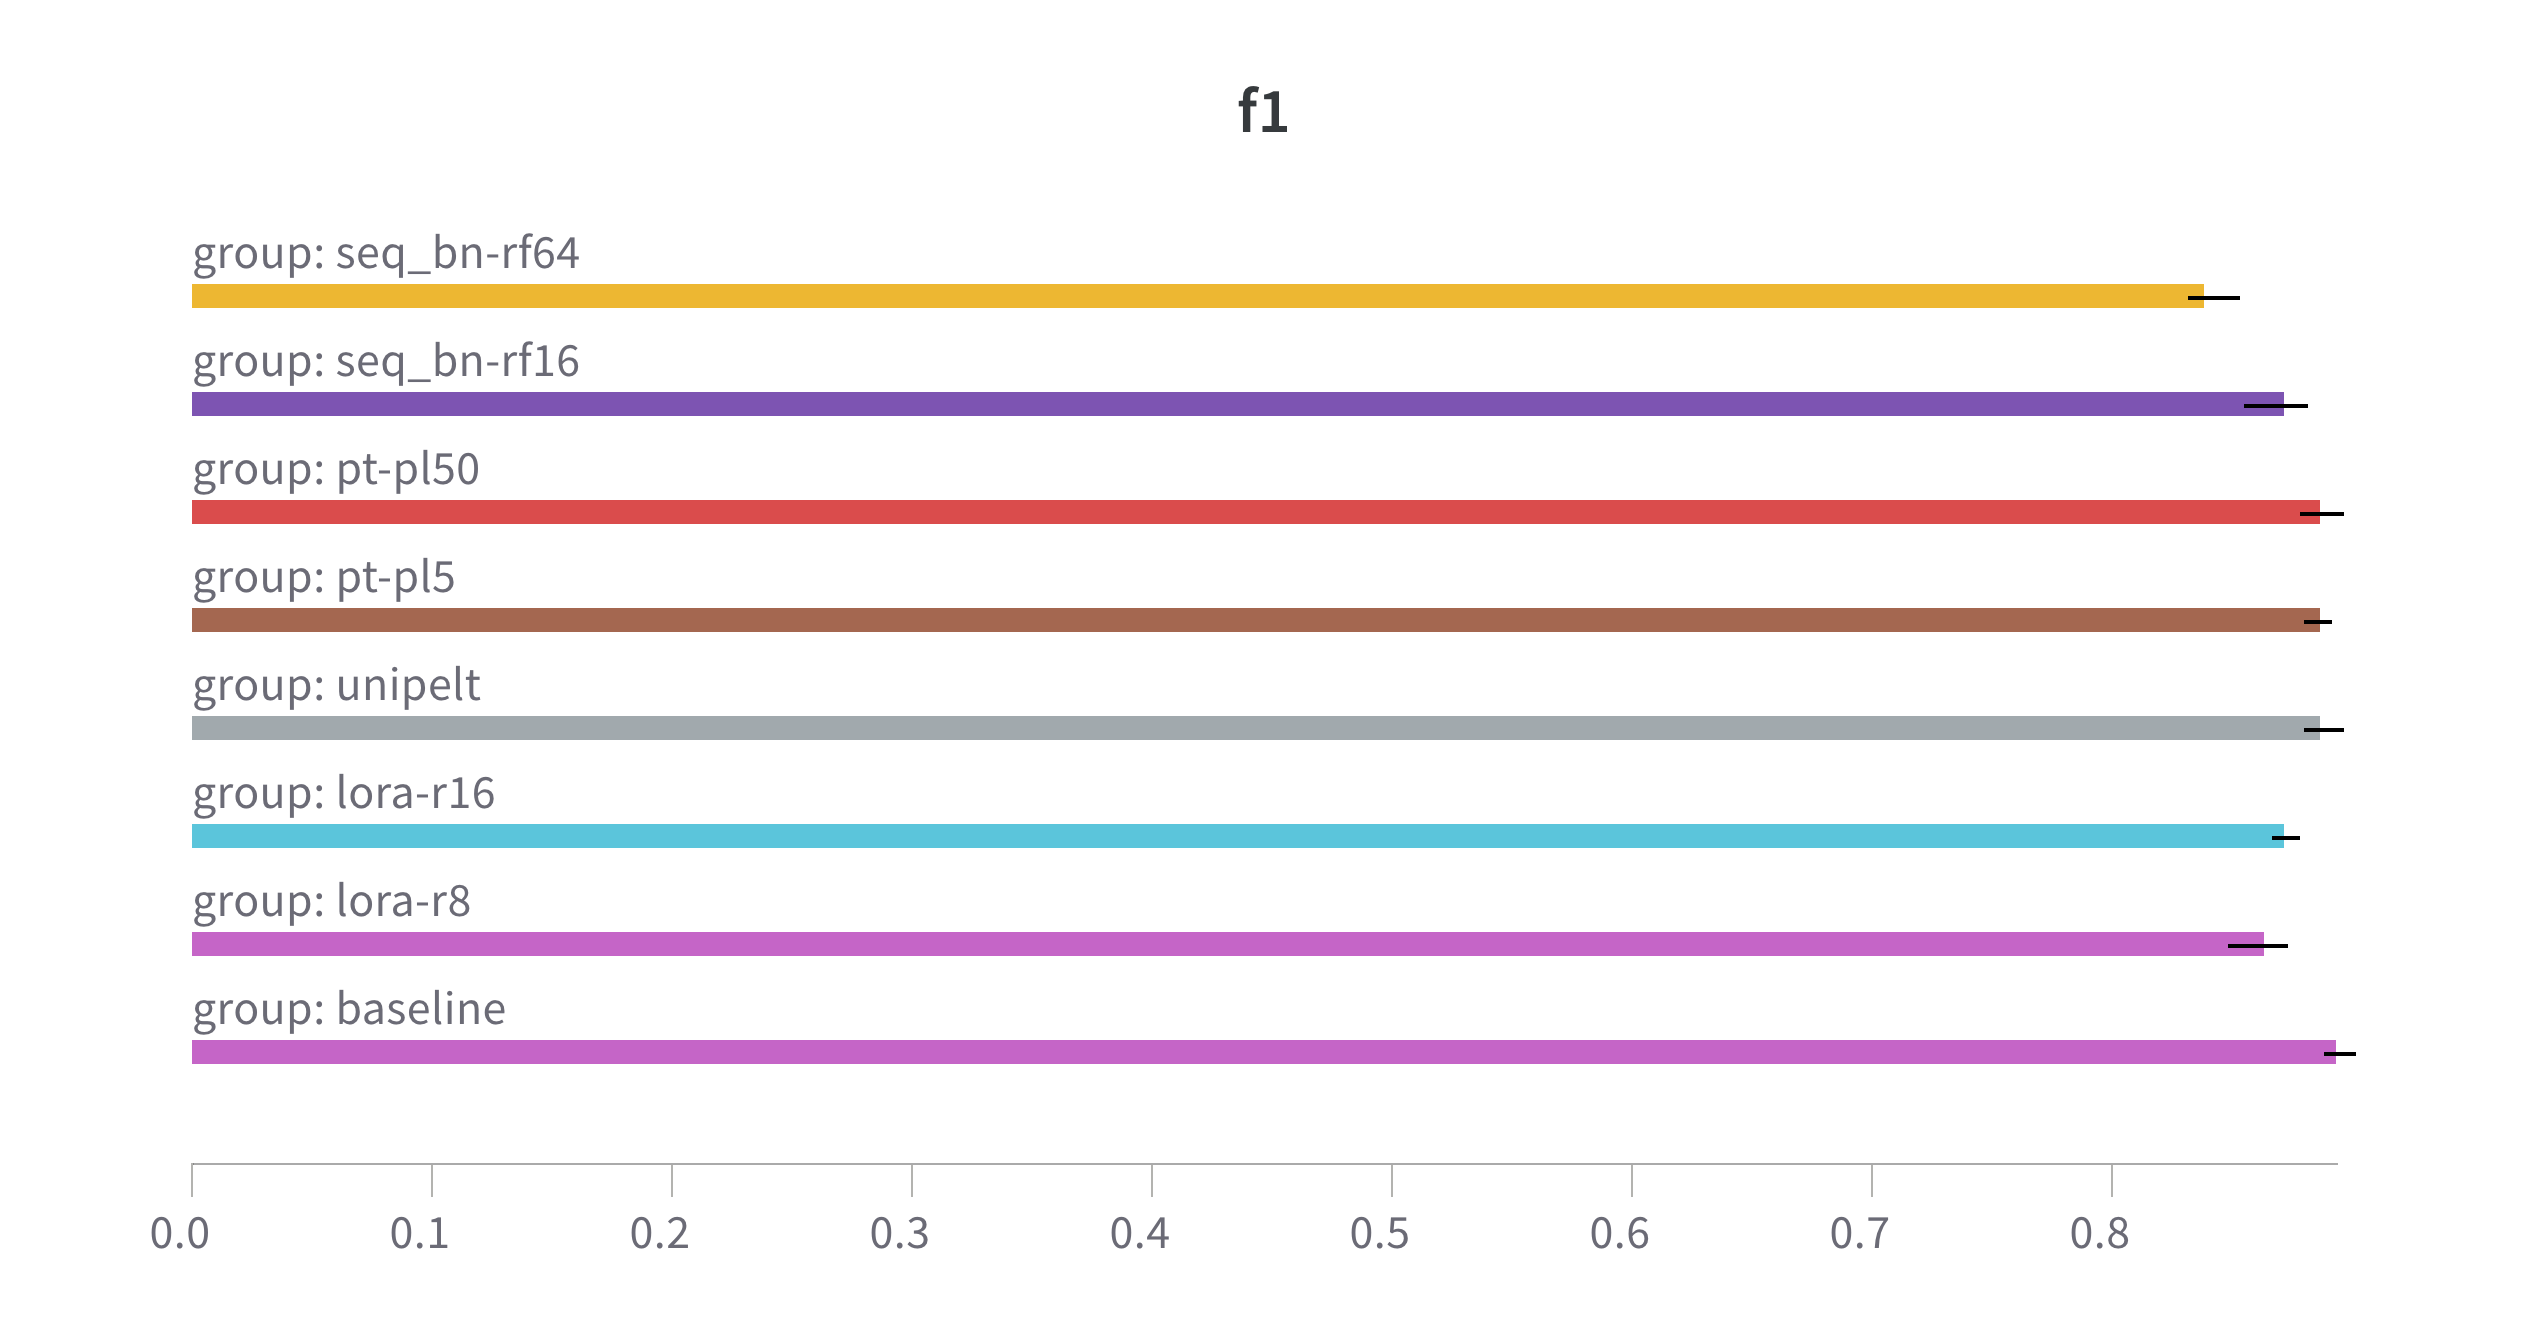
\includegraphics[width=\textwidth]{appendix/sentiment_pred_f1.png} \\
    \end{longtable}
    \caption{Hasil evaluasi dan prediksi F1 tugas \textit{sentiment analysis}}
\end{figure}

\begin{figure}[h]
    \centering
    \begin{longtable}{c}
        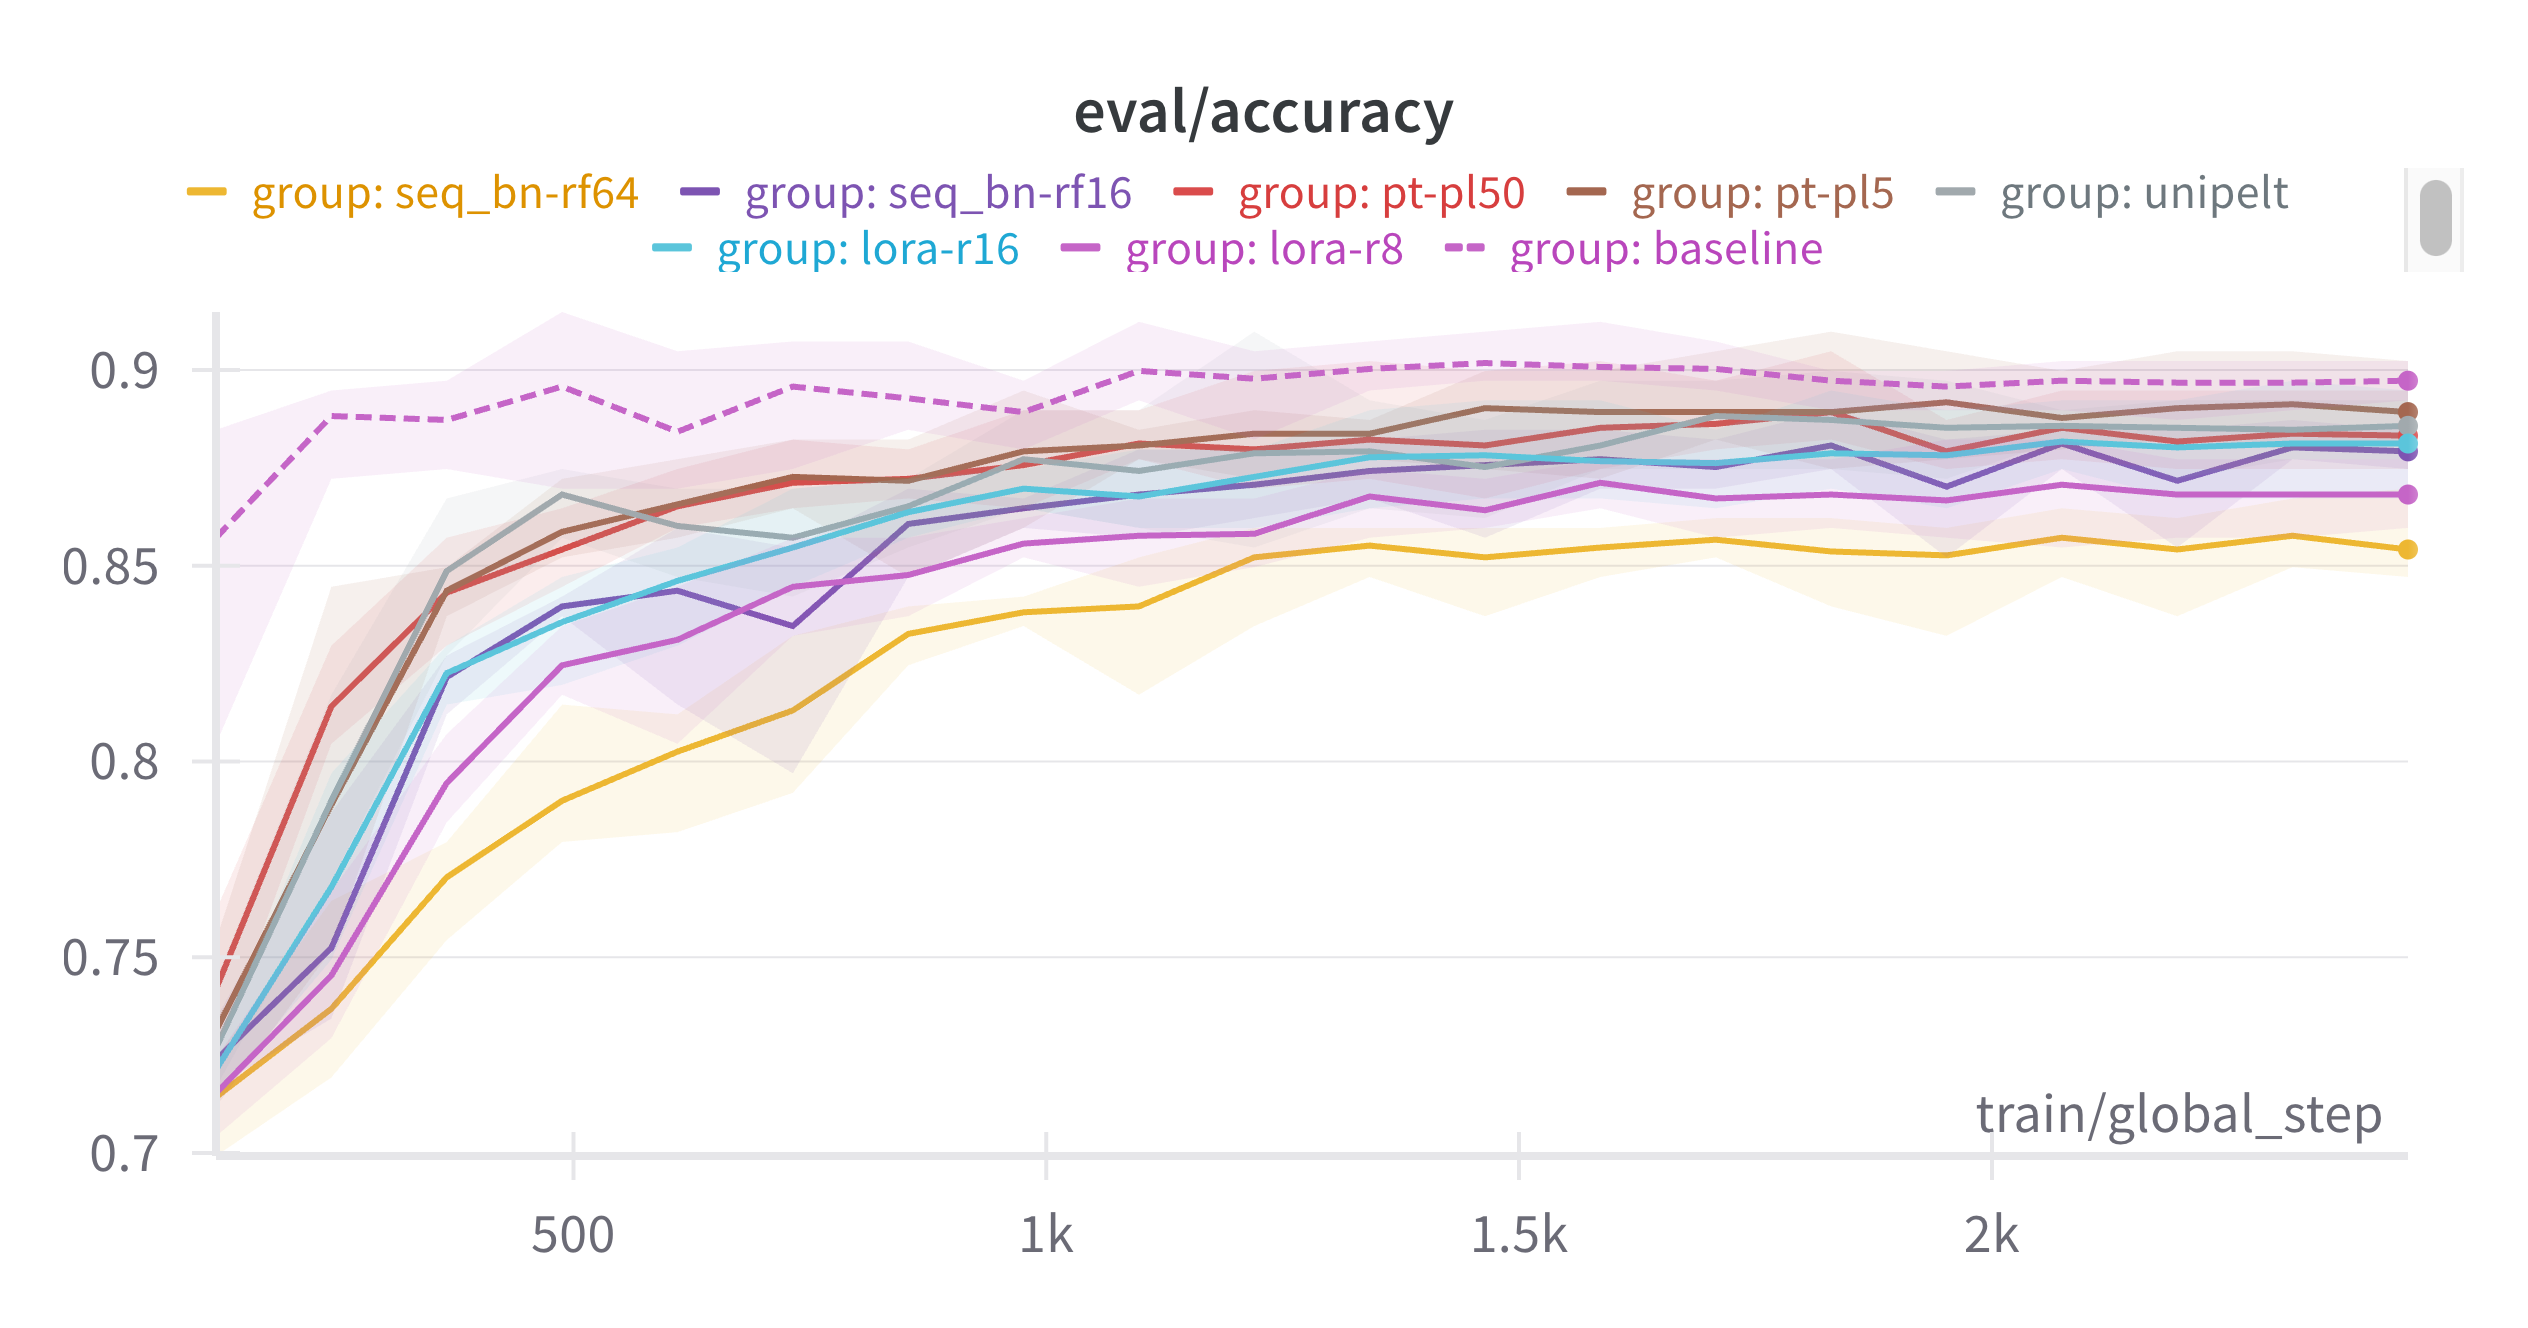
\includegraphics[width=\textwidth]{appendix/sentiment_eval_acc.png} \\
        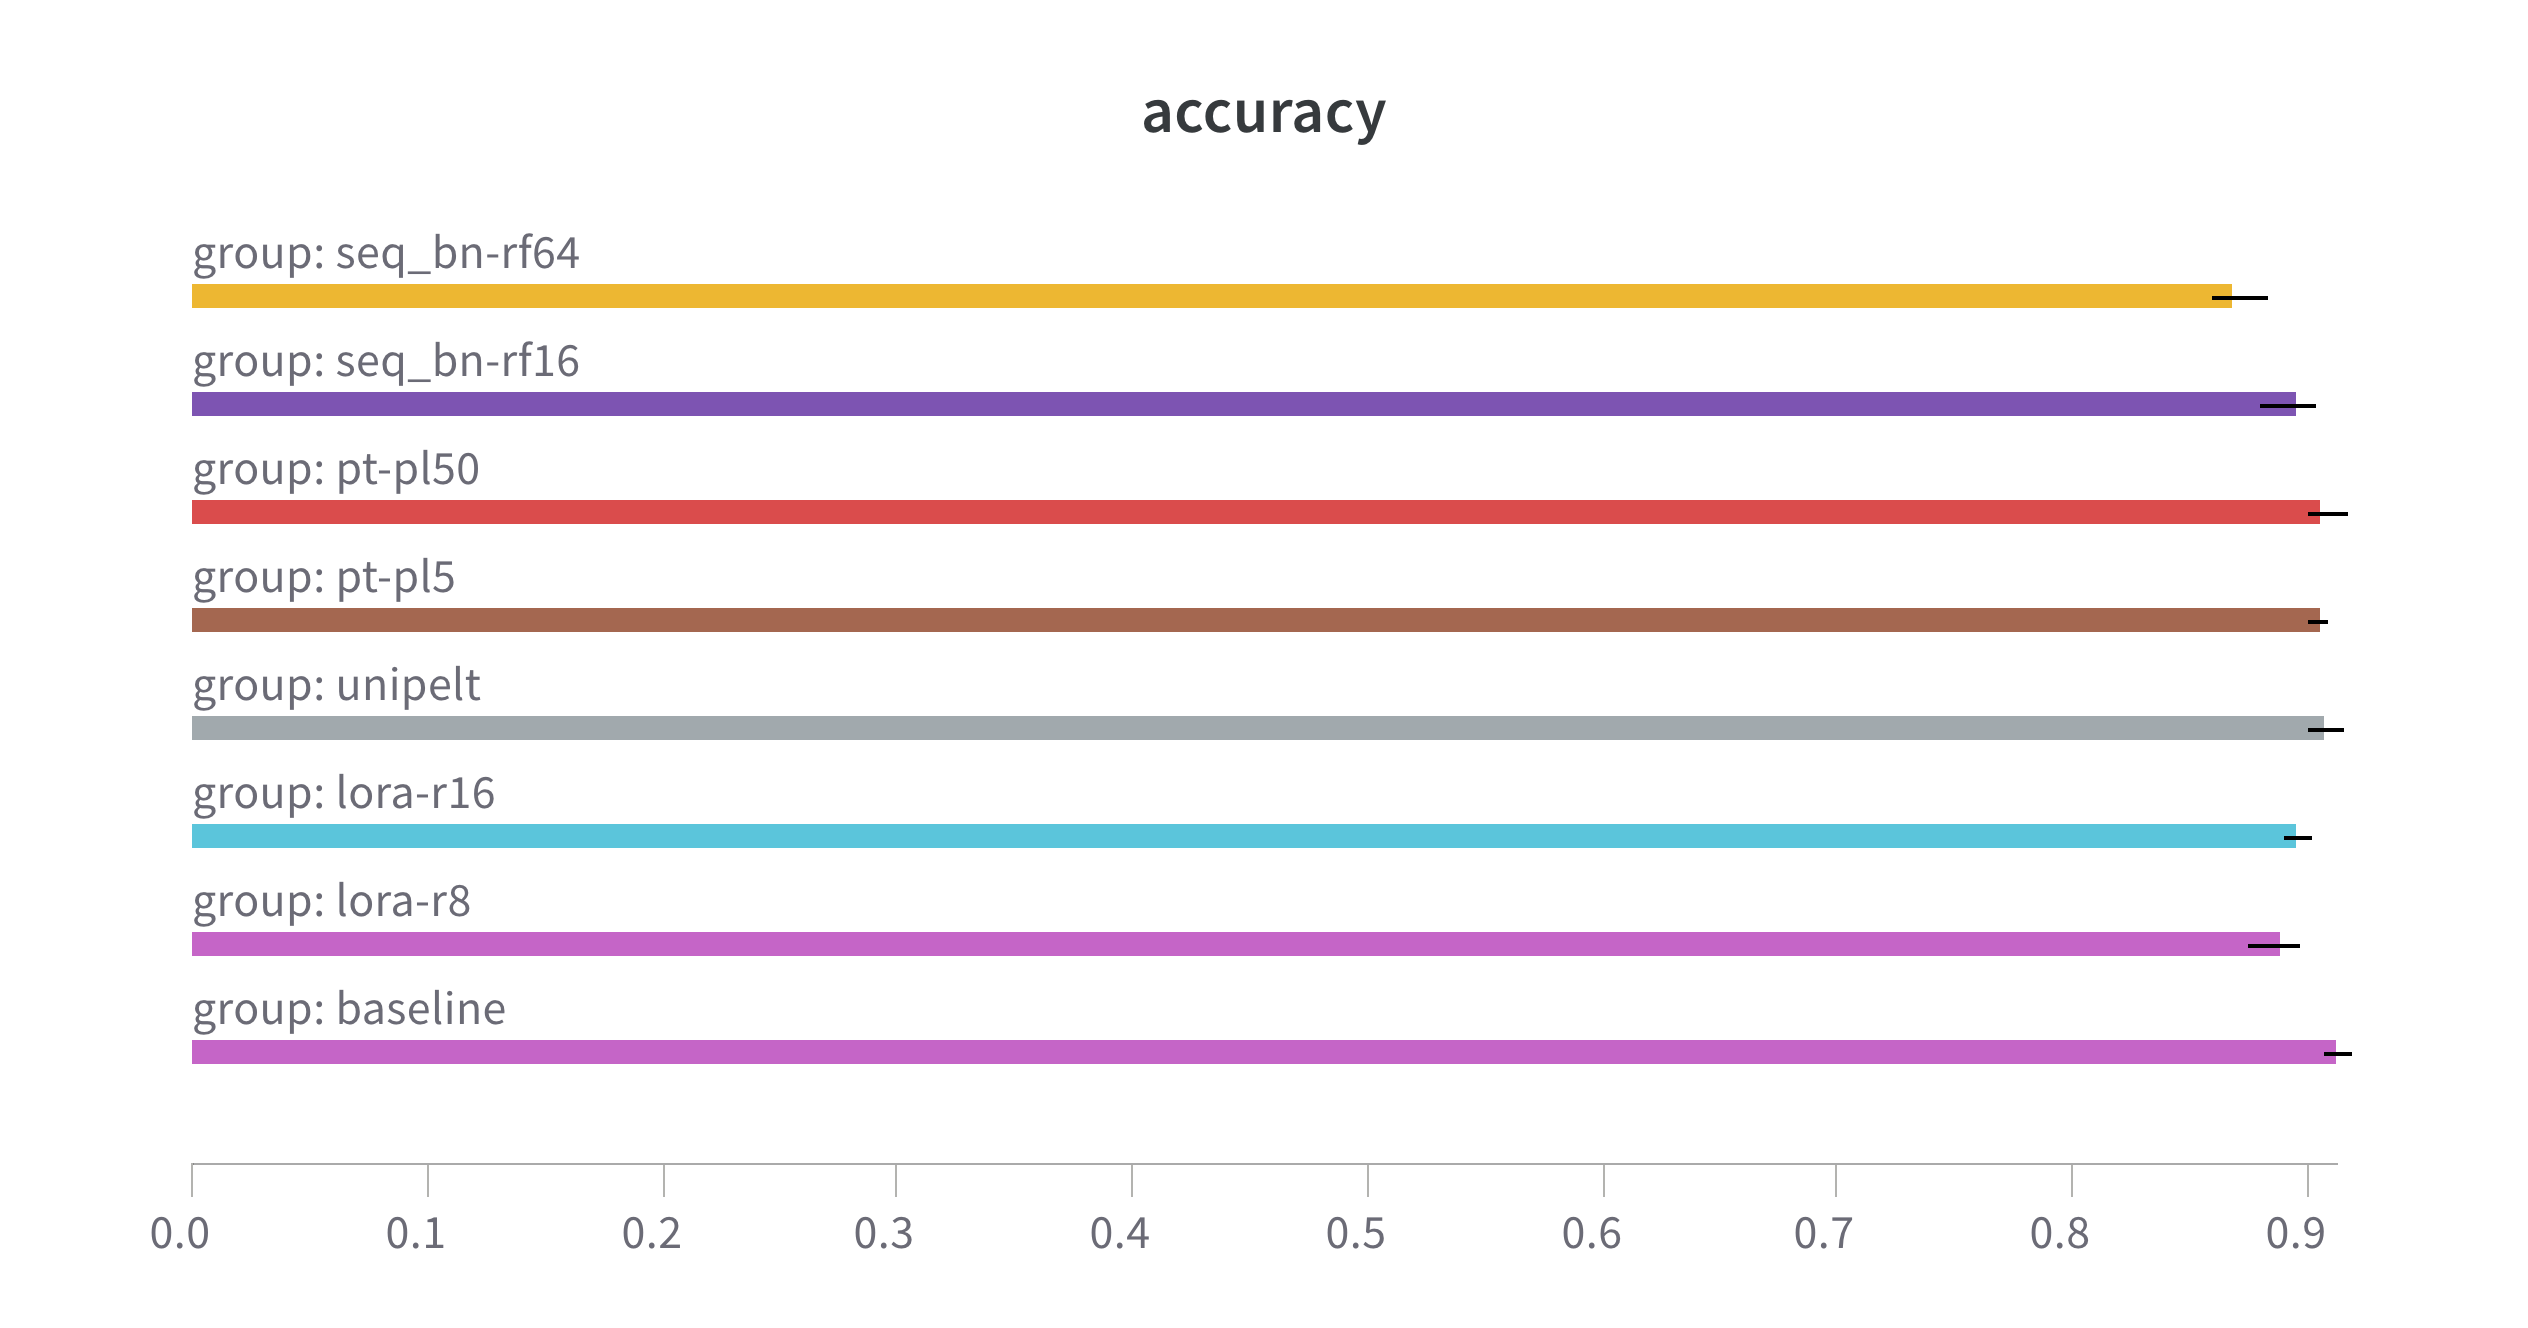
\includegraphics[width=\textwidth]{appendix/sentiment_pred_acc.png} \\
    \end{longtable}
    \caption{Hasil evaluasi dan prediksi \textit{accuracy} tugas \textit{sentiment analysis}}
\end{figure}

\begin{figure}[h]
    \centering
    \begin{longtable}{c}
        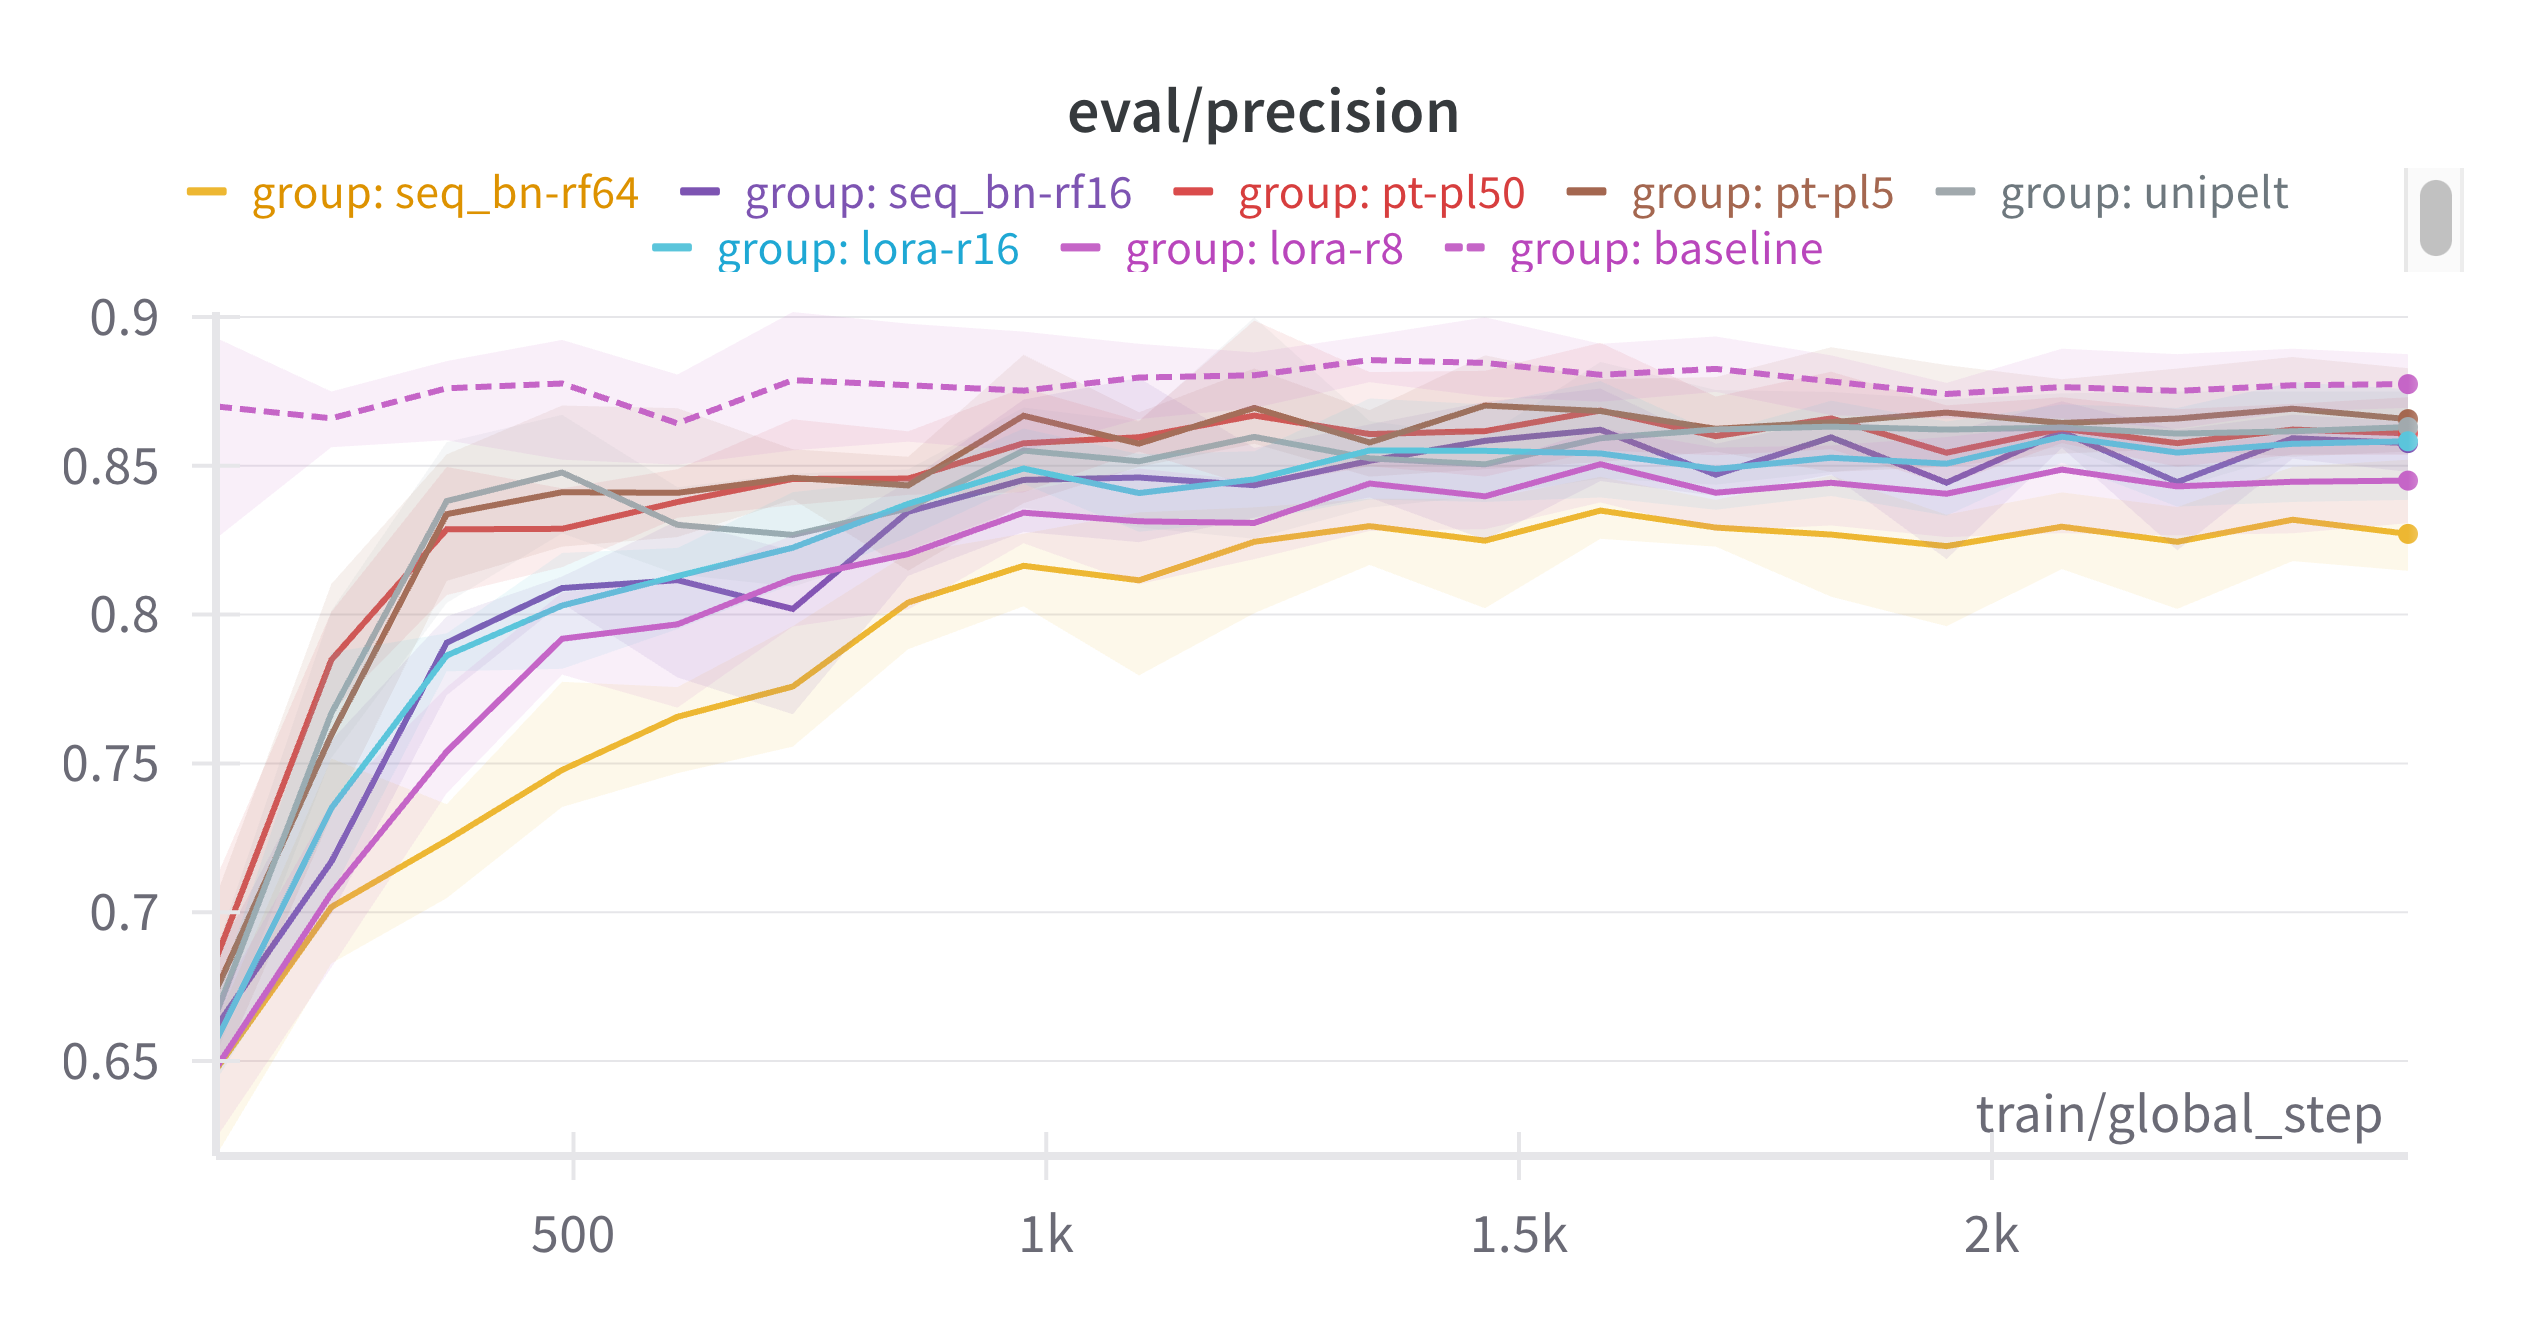
\includegraphics[width=\textwidth]{appendix/sentiment_eval_precision.png} \\
        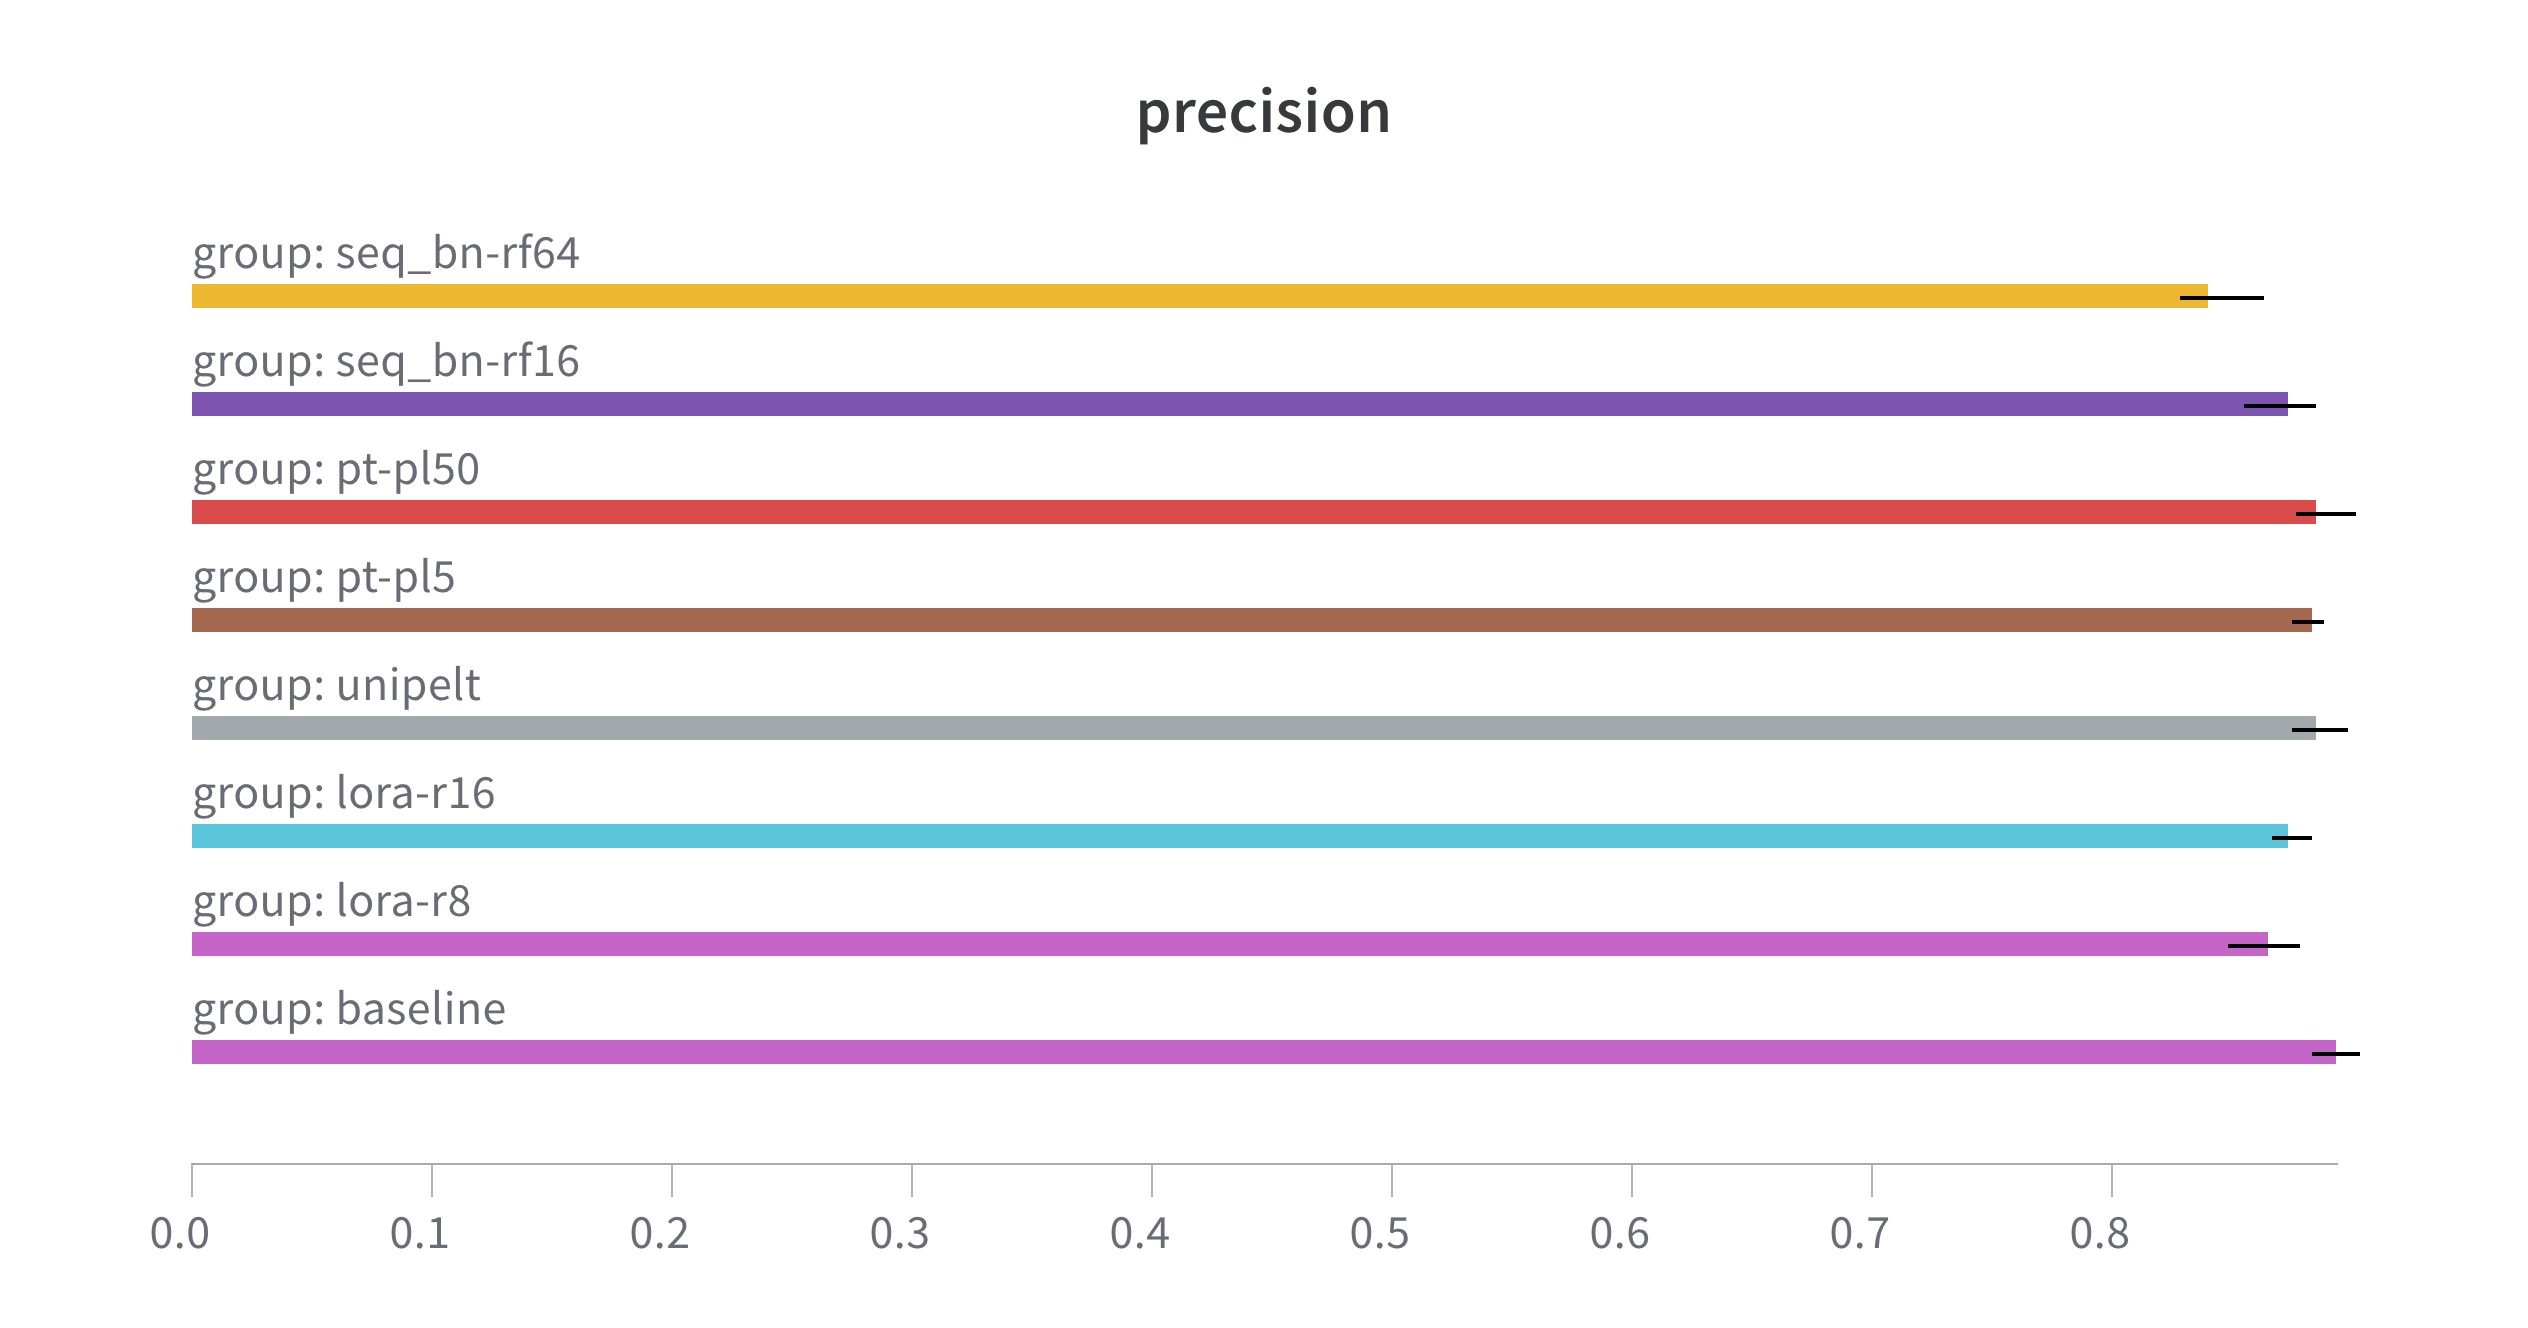
\includegraphics[width=\textwidth]{appendix/sentiment_pred_precision.png} \\
    \end{longtable}
    \caption{Hasil evaluasi dan prediksi \textit{precision} tugas \textit{sentiment analysis}}
\end{figure}

\begin{figure}[h]
    \centering
    \begin{longtable}{c}
        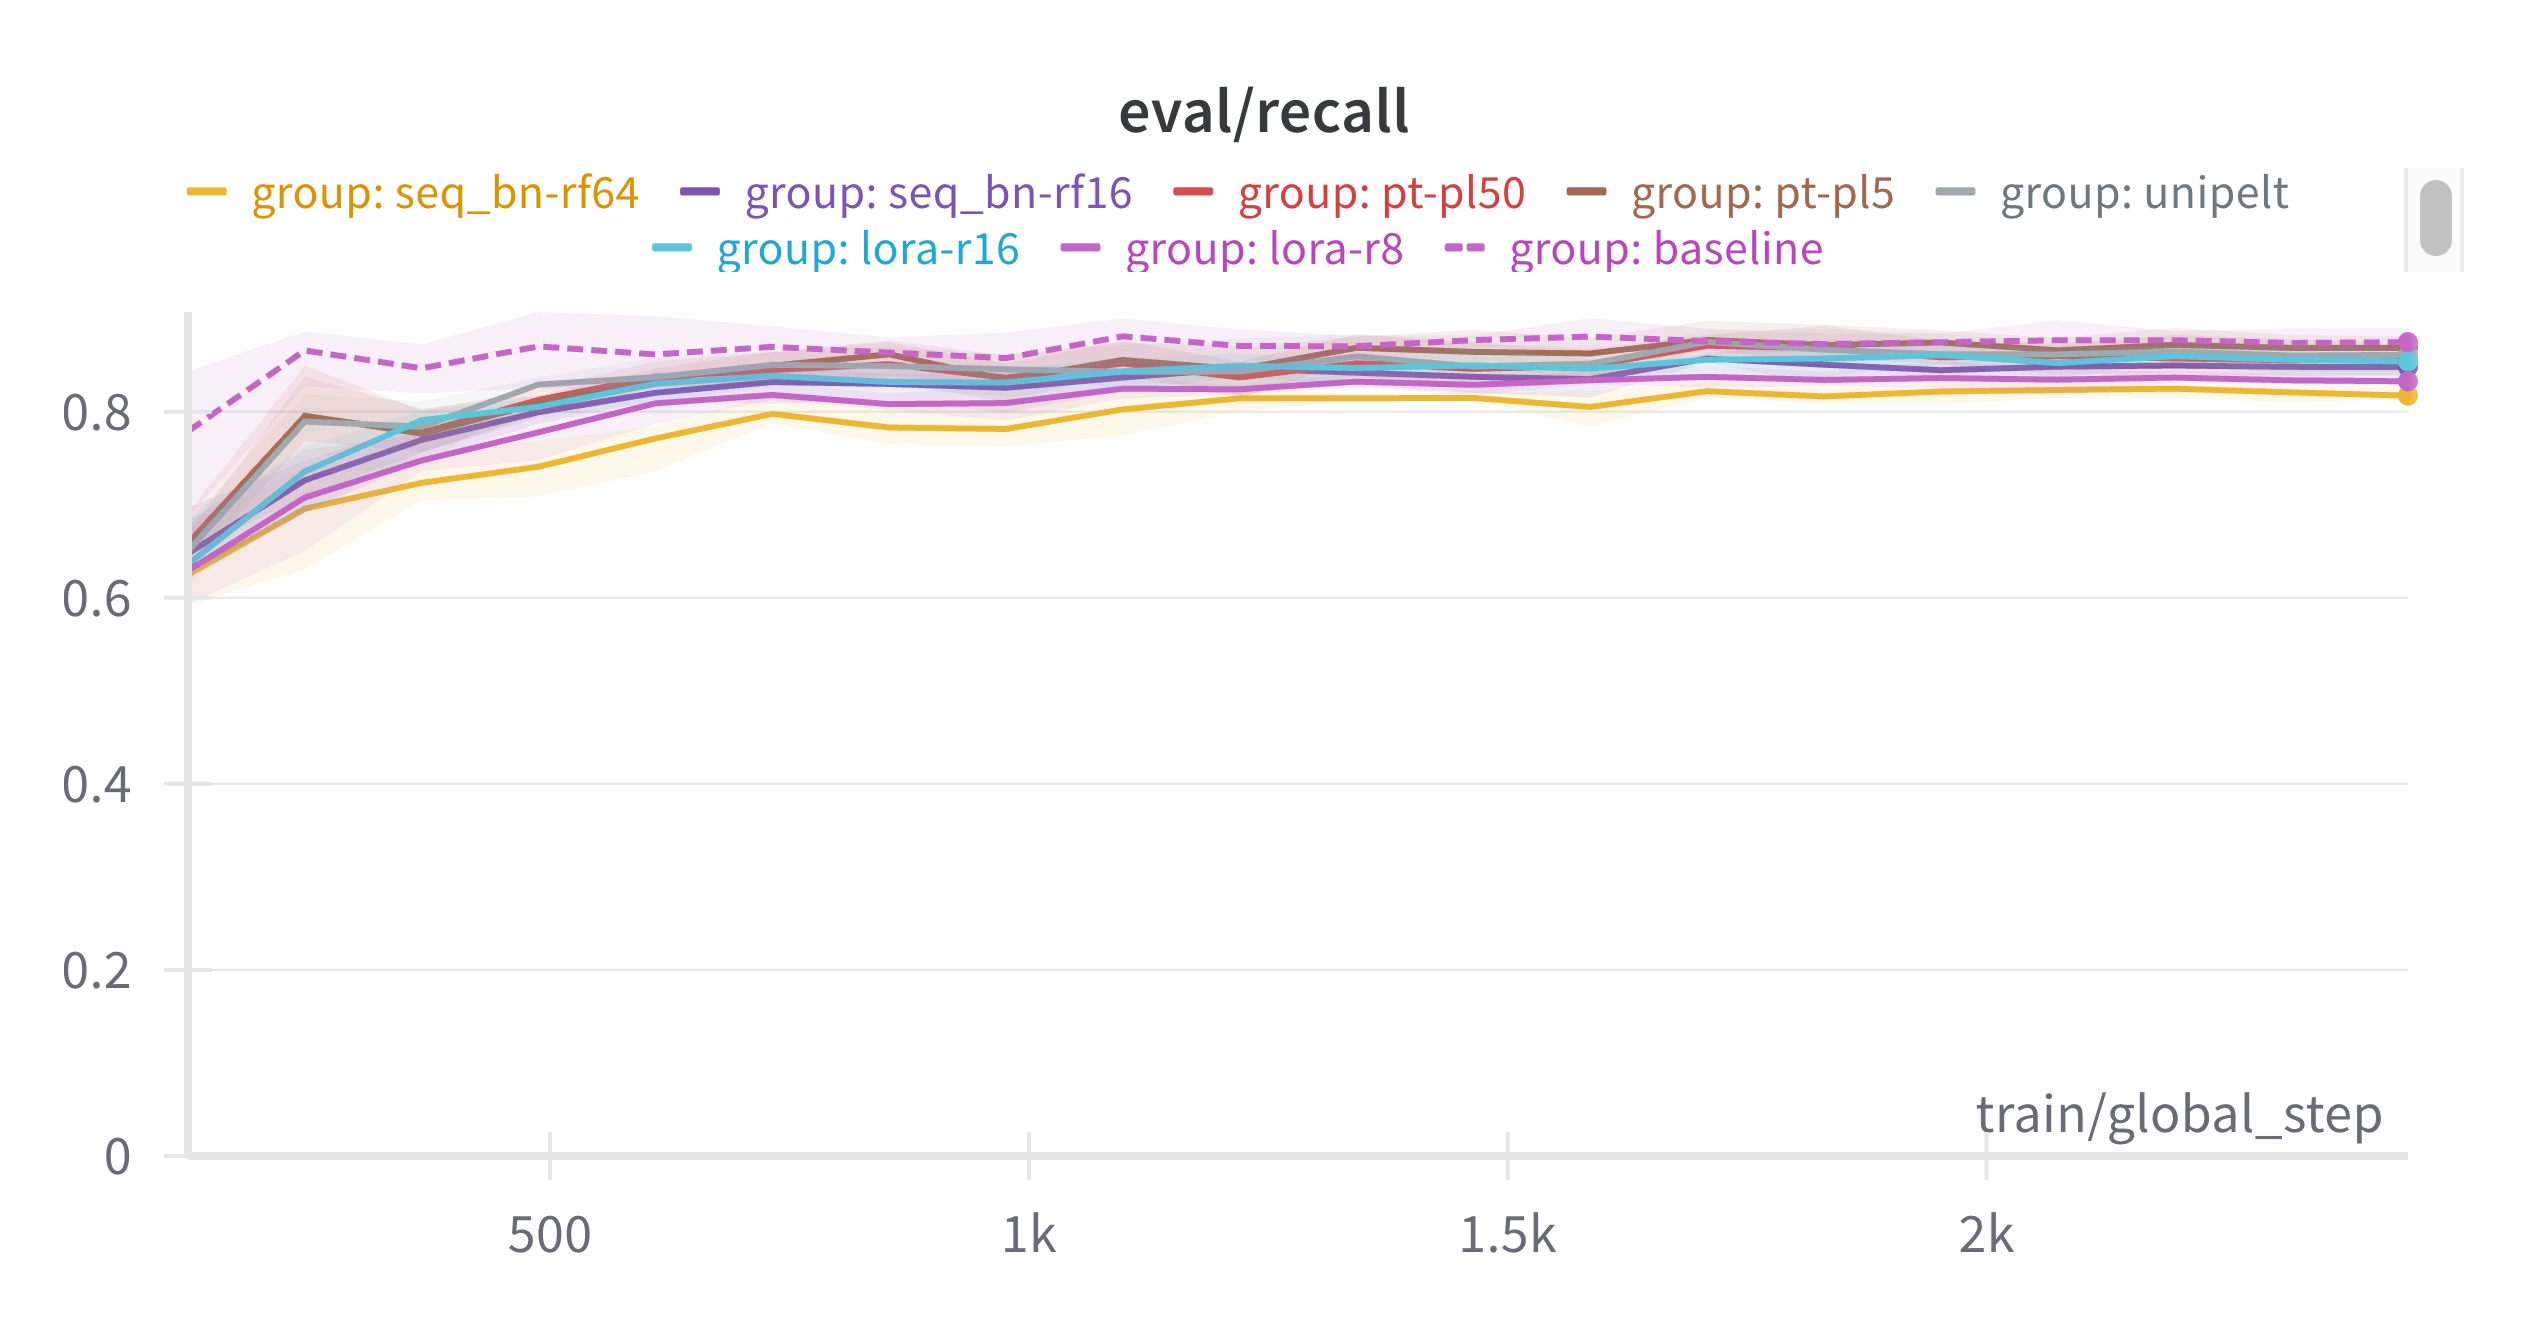
\includegraphics[width=\textwidth]{appendix/sentiment_eval_recall.png} \\
        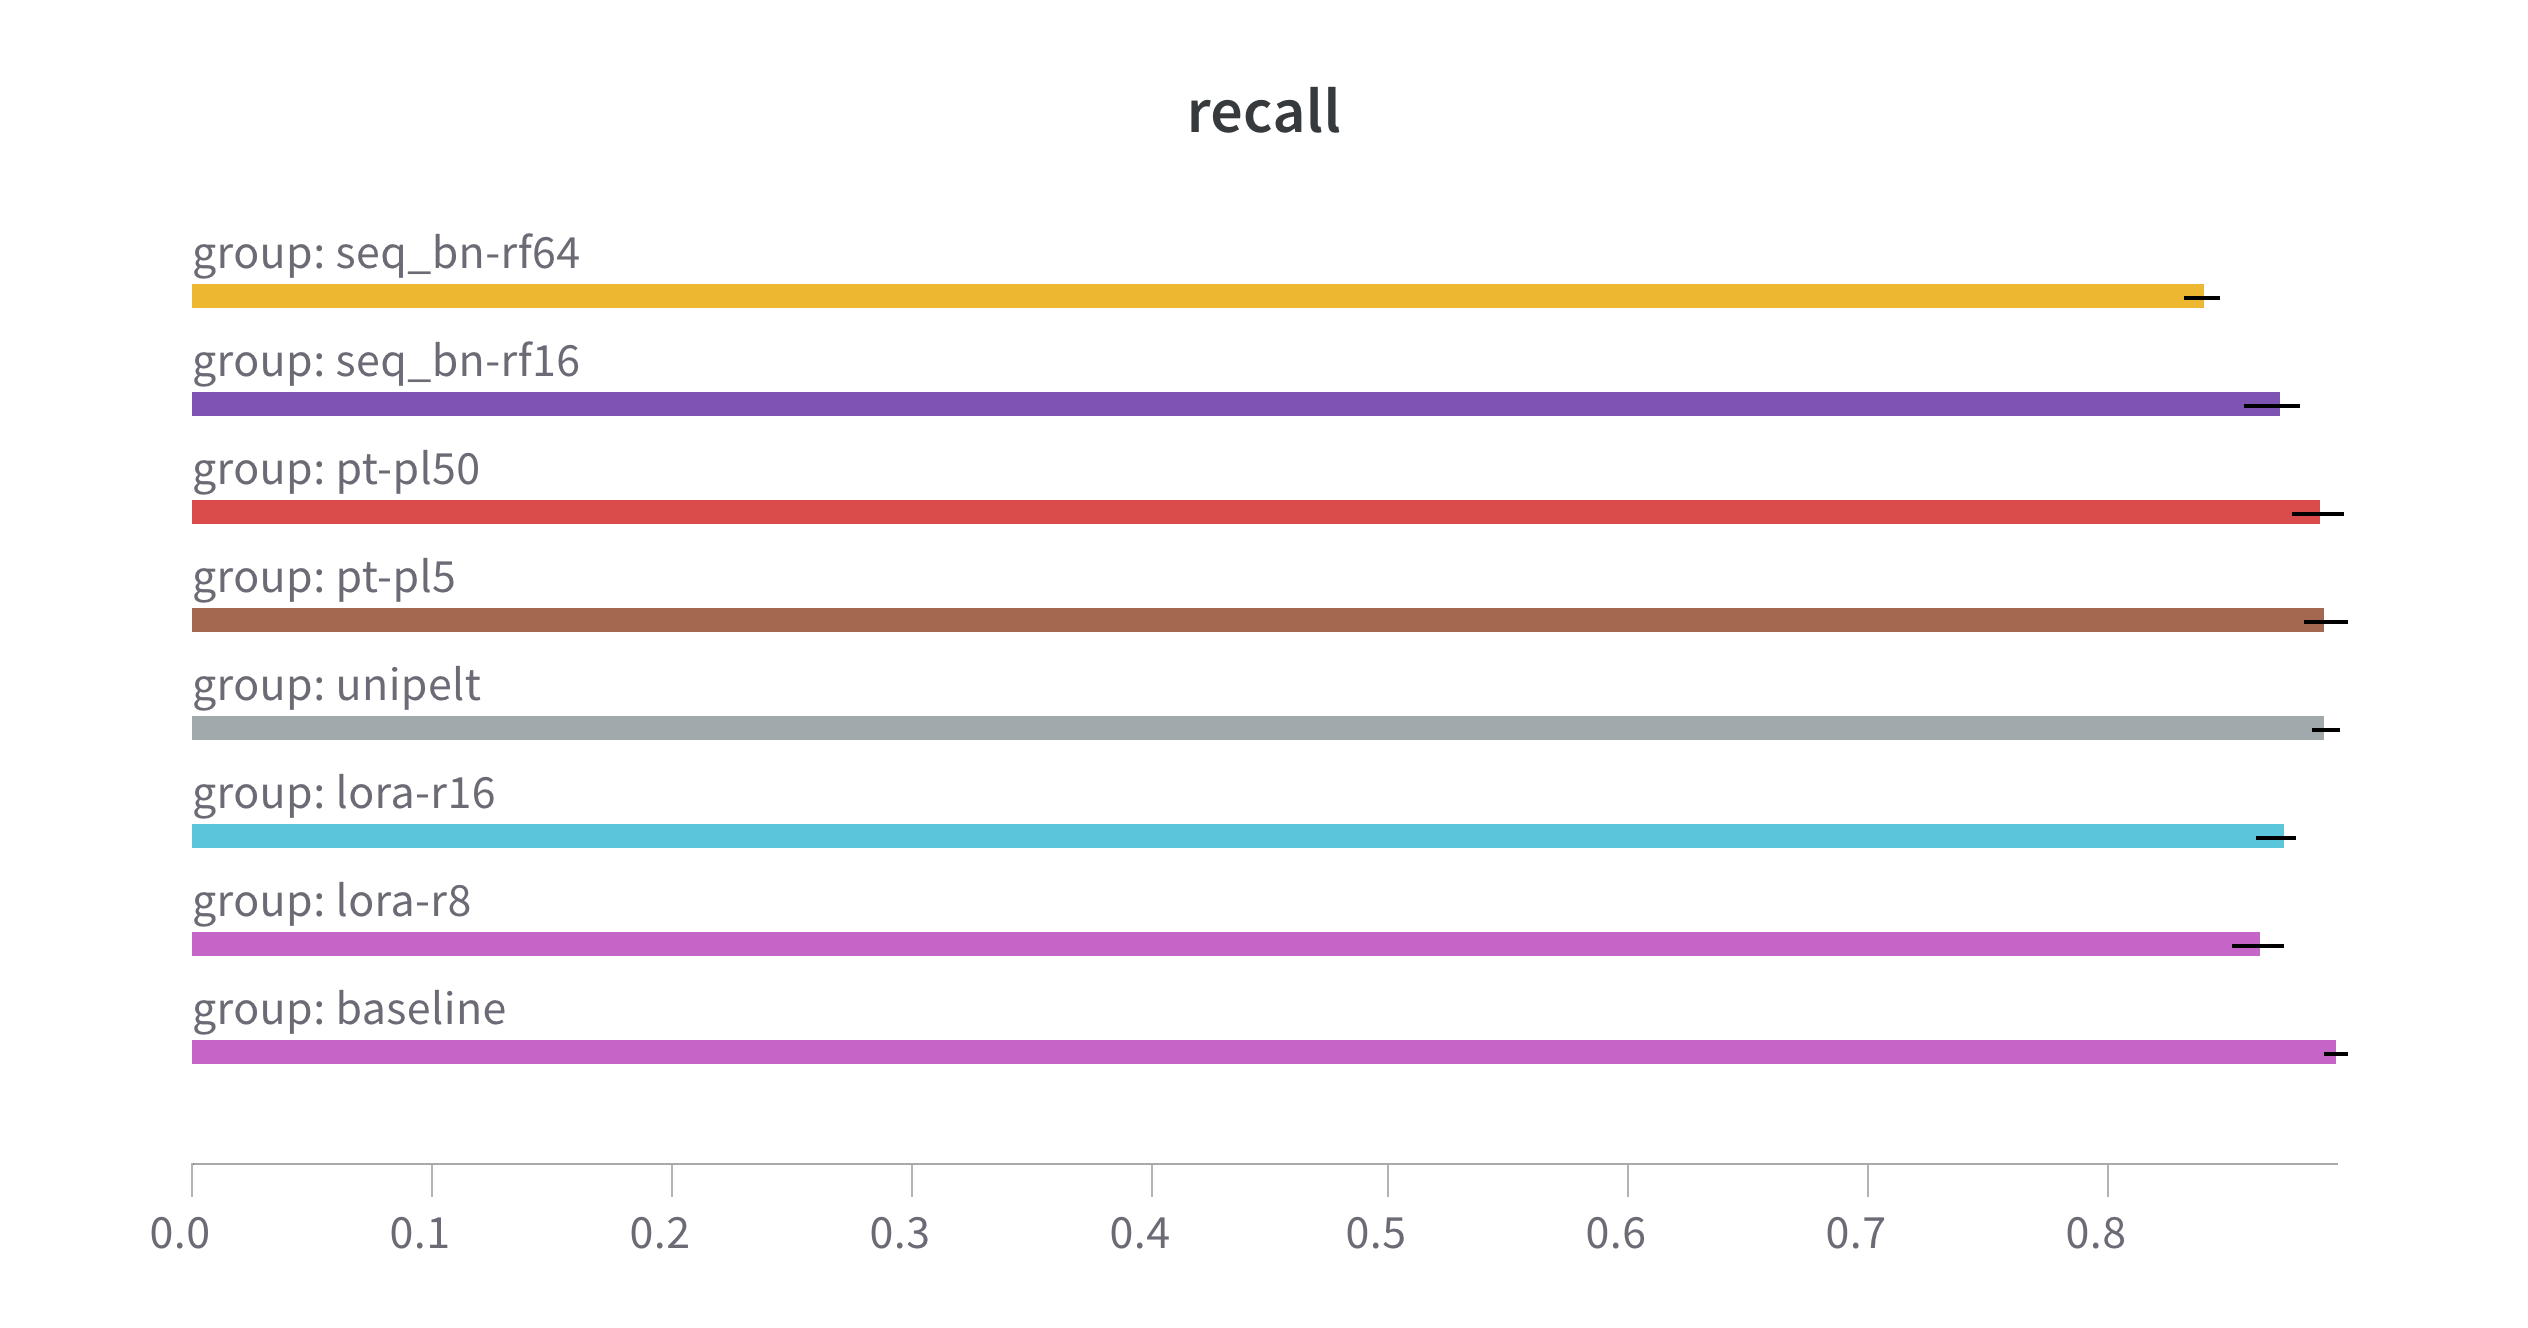
\includegraphics[width=\textwidth]{appendix/sentiment_pred_recall.png} \\
    \end{longtable}
    \caption{Hasil evaluasi dan prediksi \textit{recall} tugas \textit{sentiment analysis}}
\end{figure}

\chapter{Hasil Evaluasi dan Prediksi Tugas \textit{Summarization}}
\label{appendix:summarization}

\begin{figure}[h]
    \centering
    \begin{longtable}{c}
        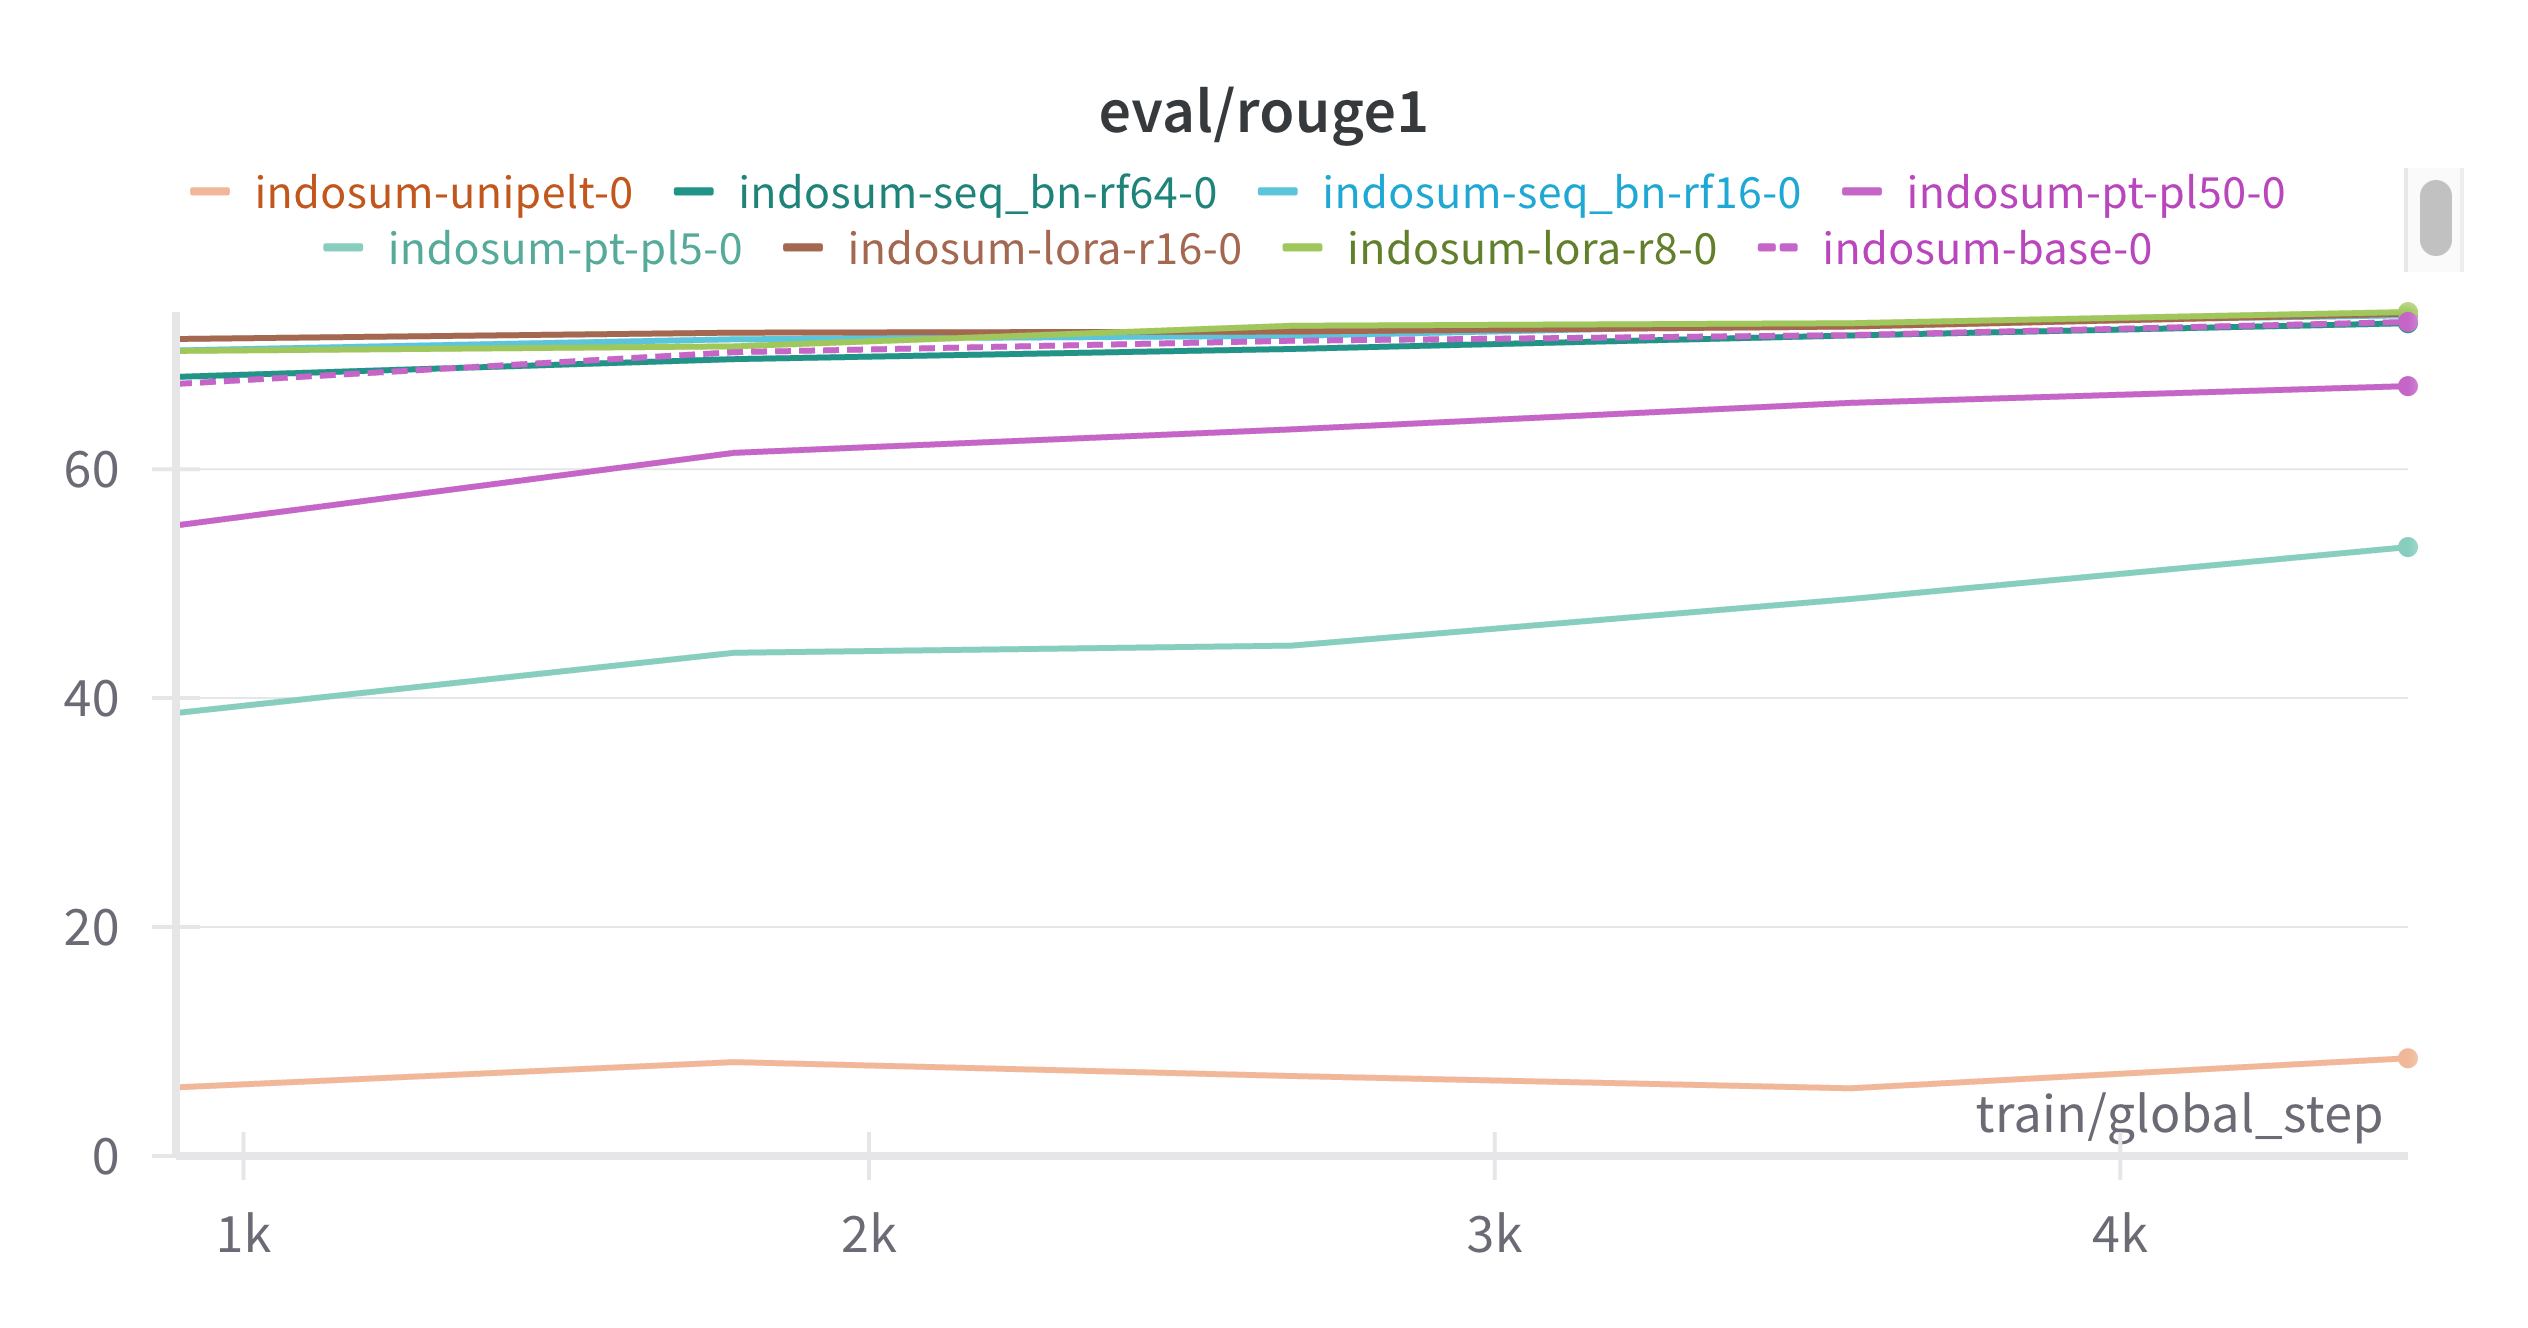
\includegraphics[width=\textwidth]{appendix/summ_eval_r1.png} \\
        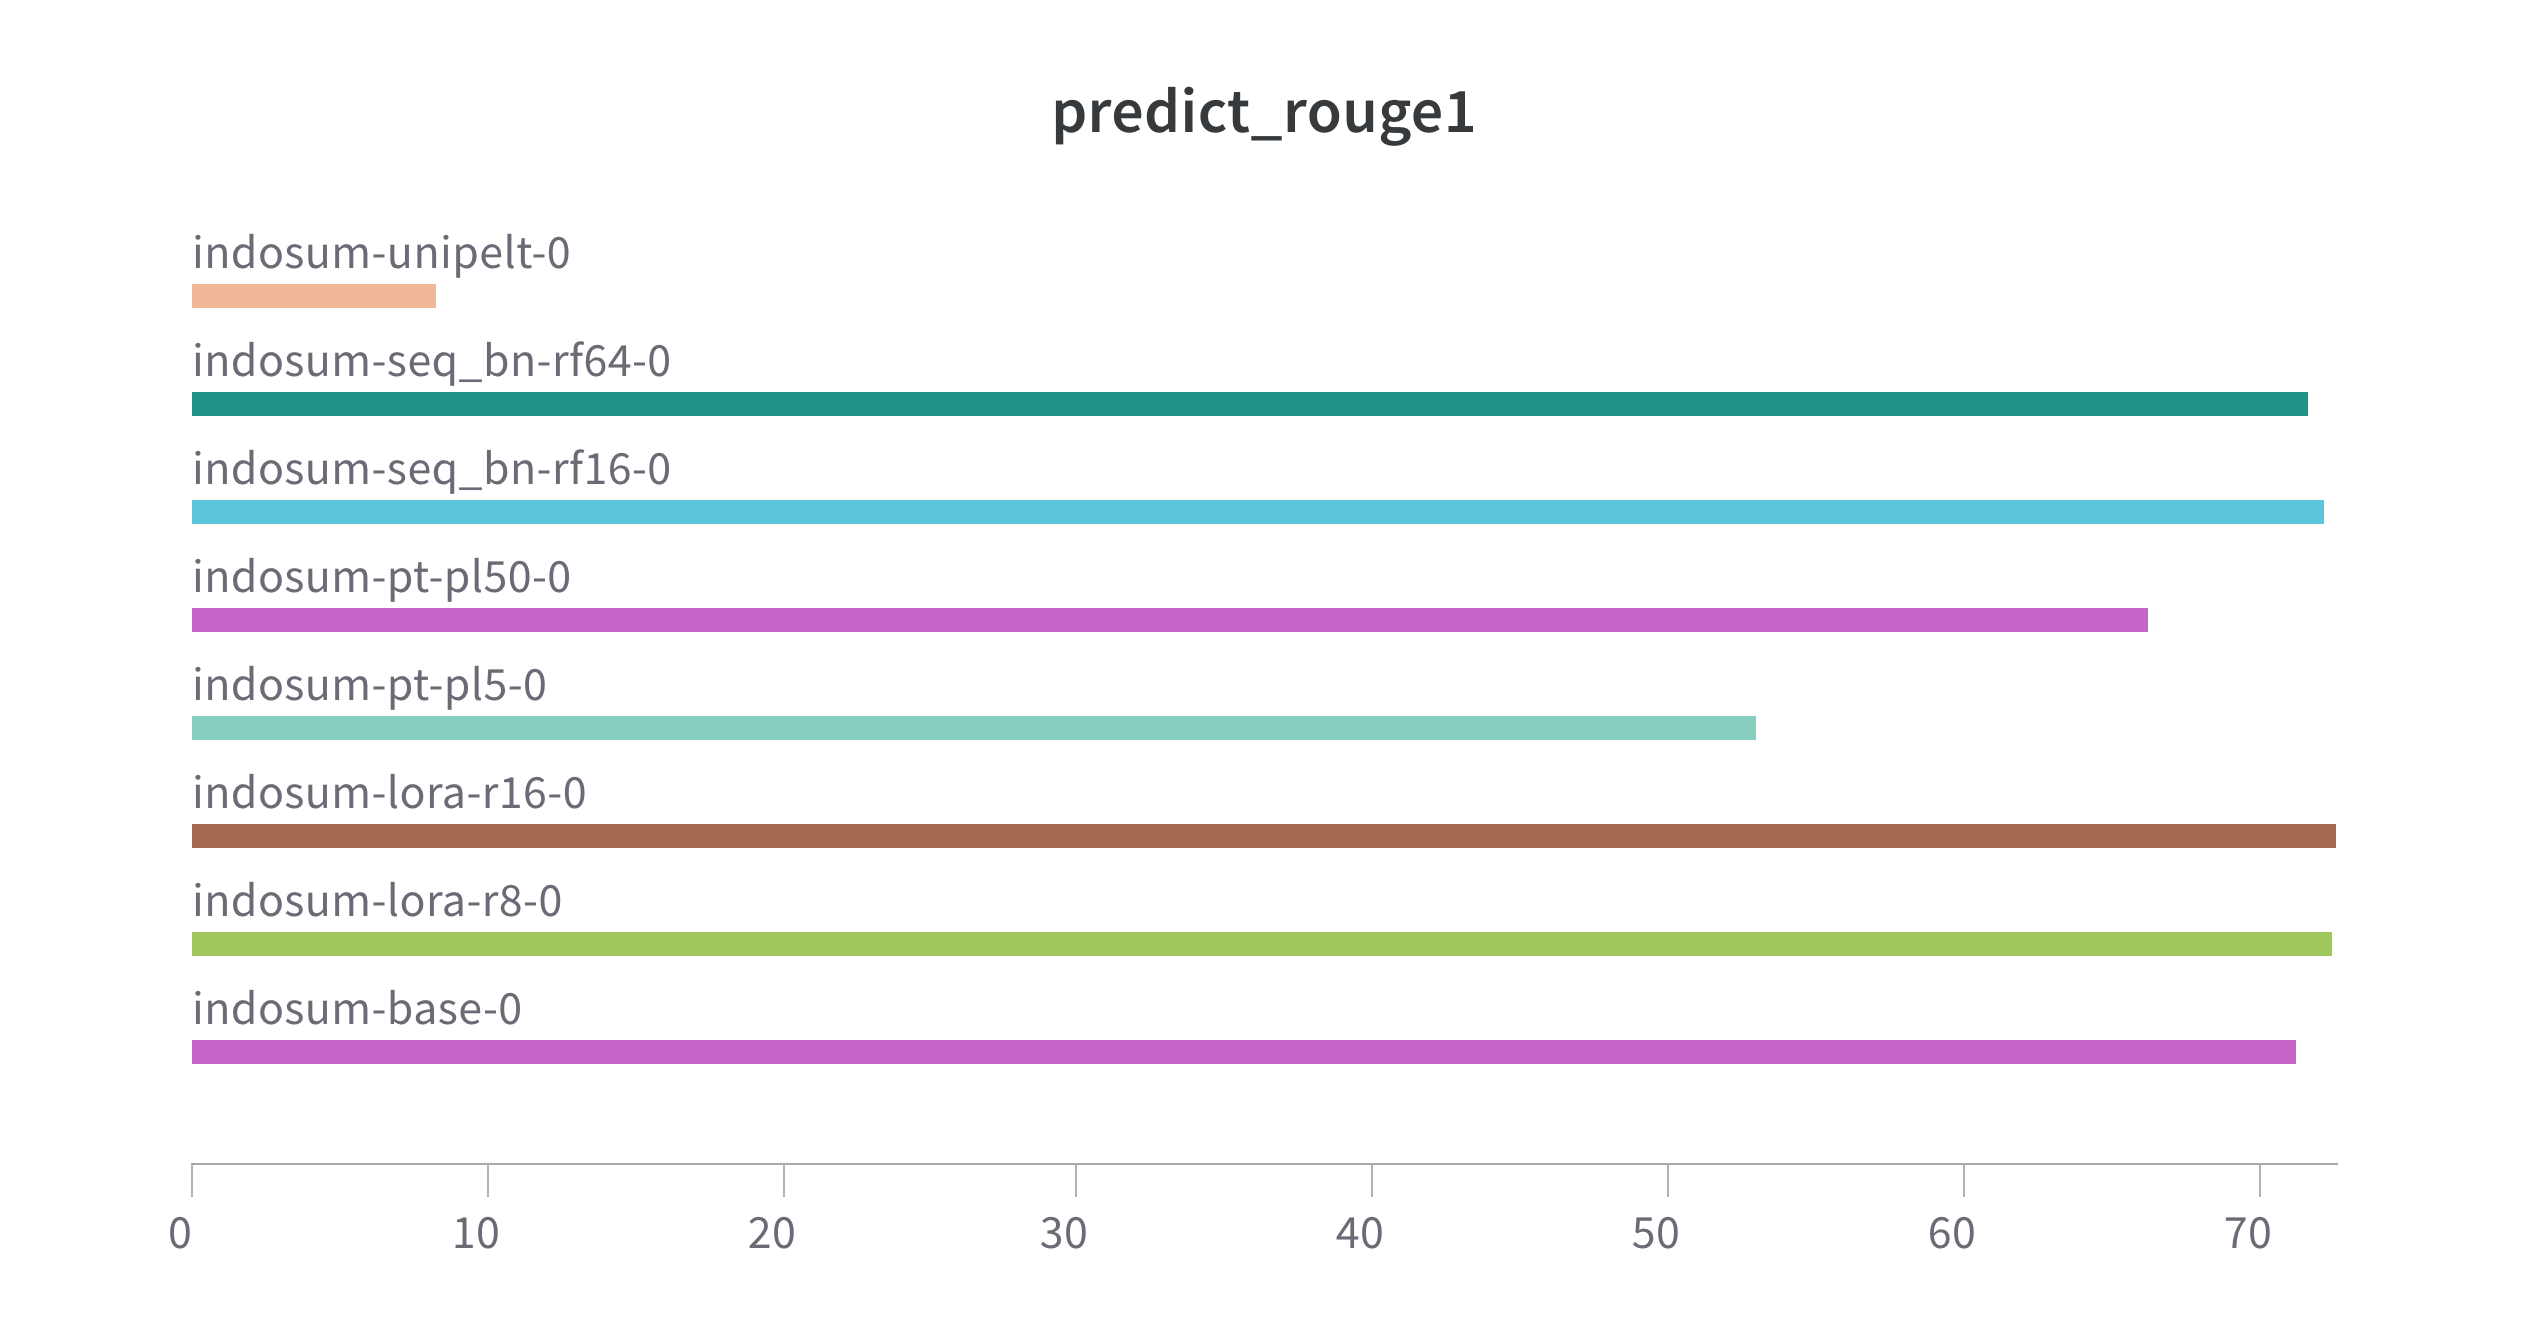
\includegraphics[width=\textwidth]{appendix/summ_pred_r1.png} \\
    \end{longtable}
    \caption{Hasil evaluasi dan prediksi ROUGE-1 tugas \textit{summarization}}
\end{figure}

\begin{figure}[h]
    \centering
    \begin{longtable}{c}
        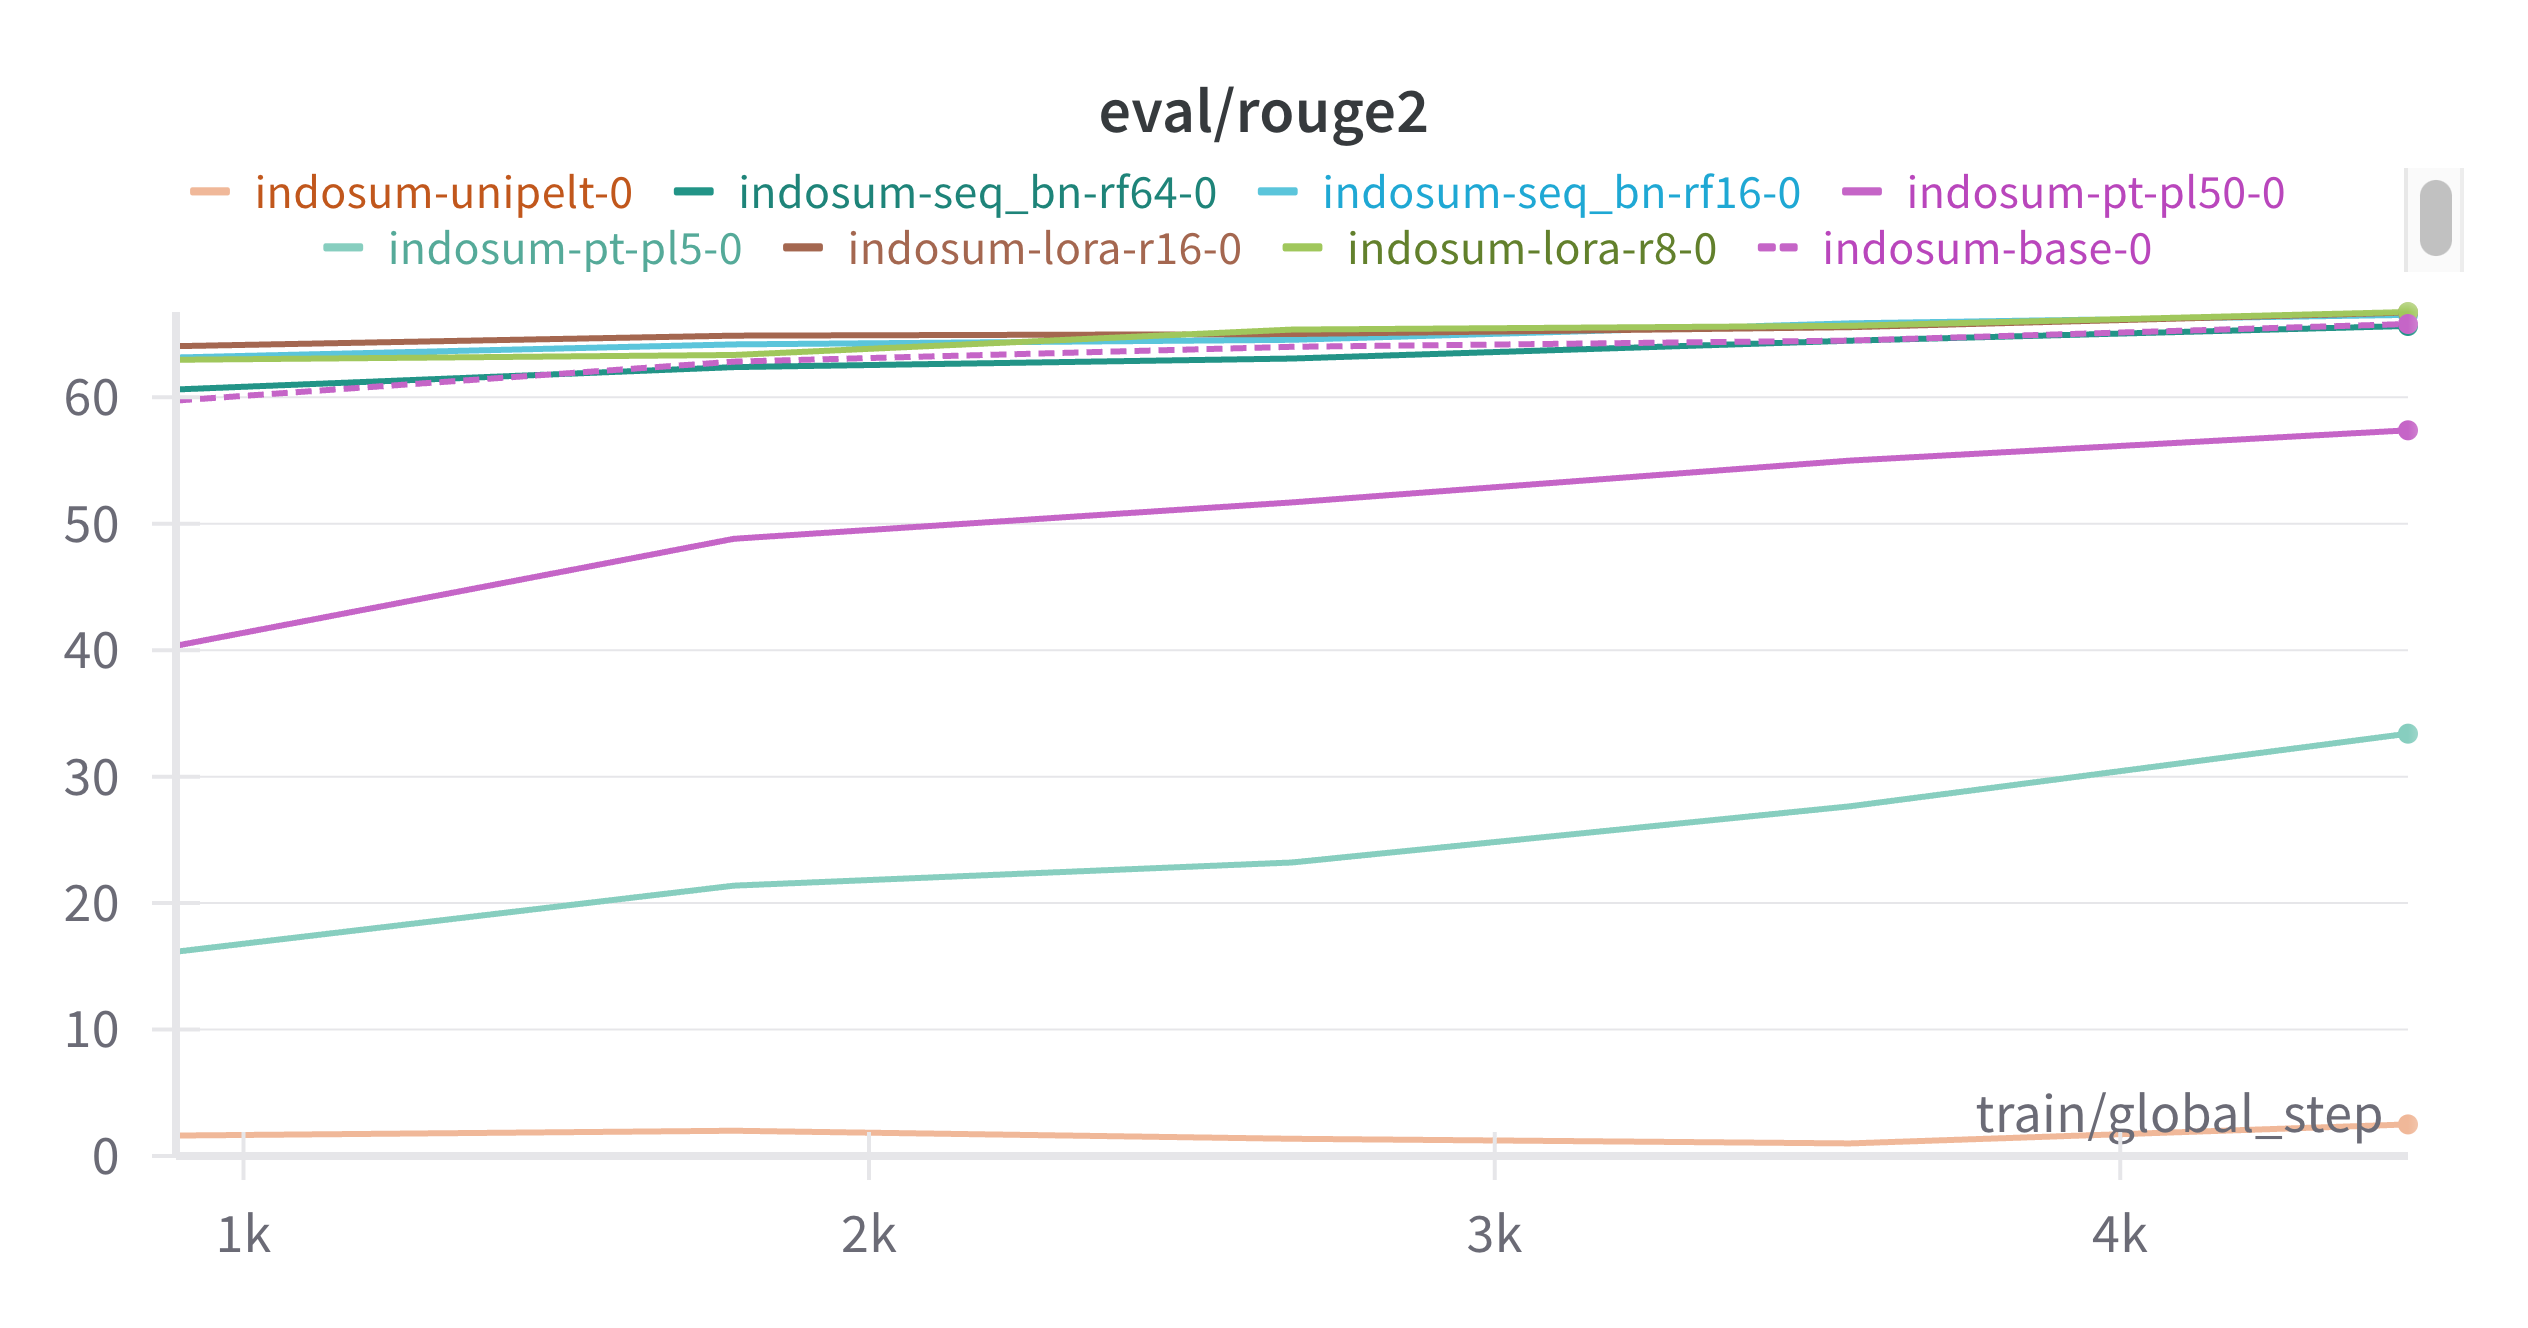
\includegraphics[width=\textwidth]{appendix/summ_eval_r2.png} \\
        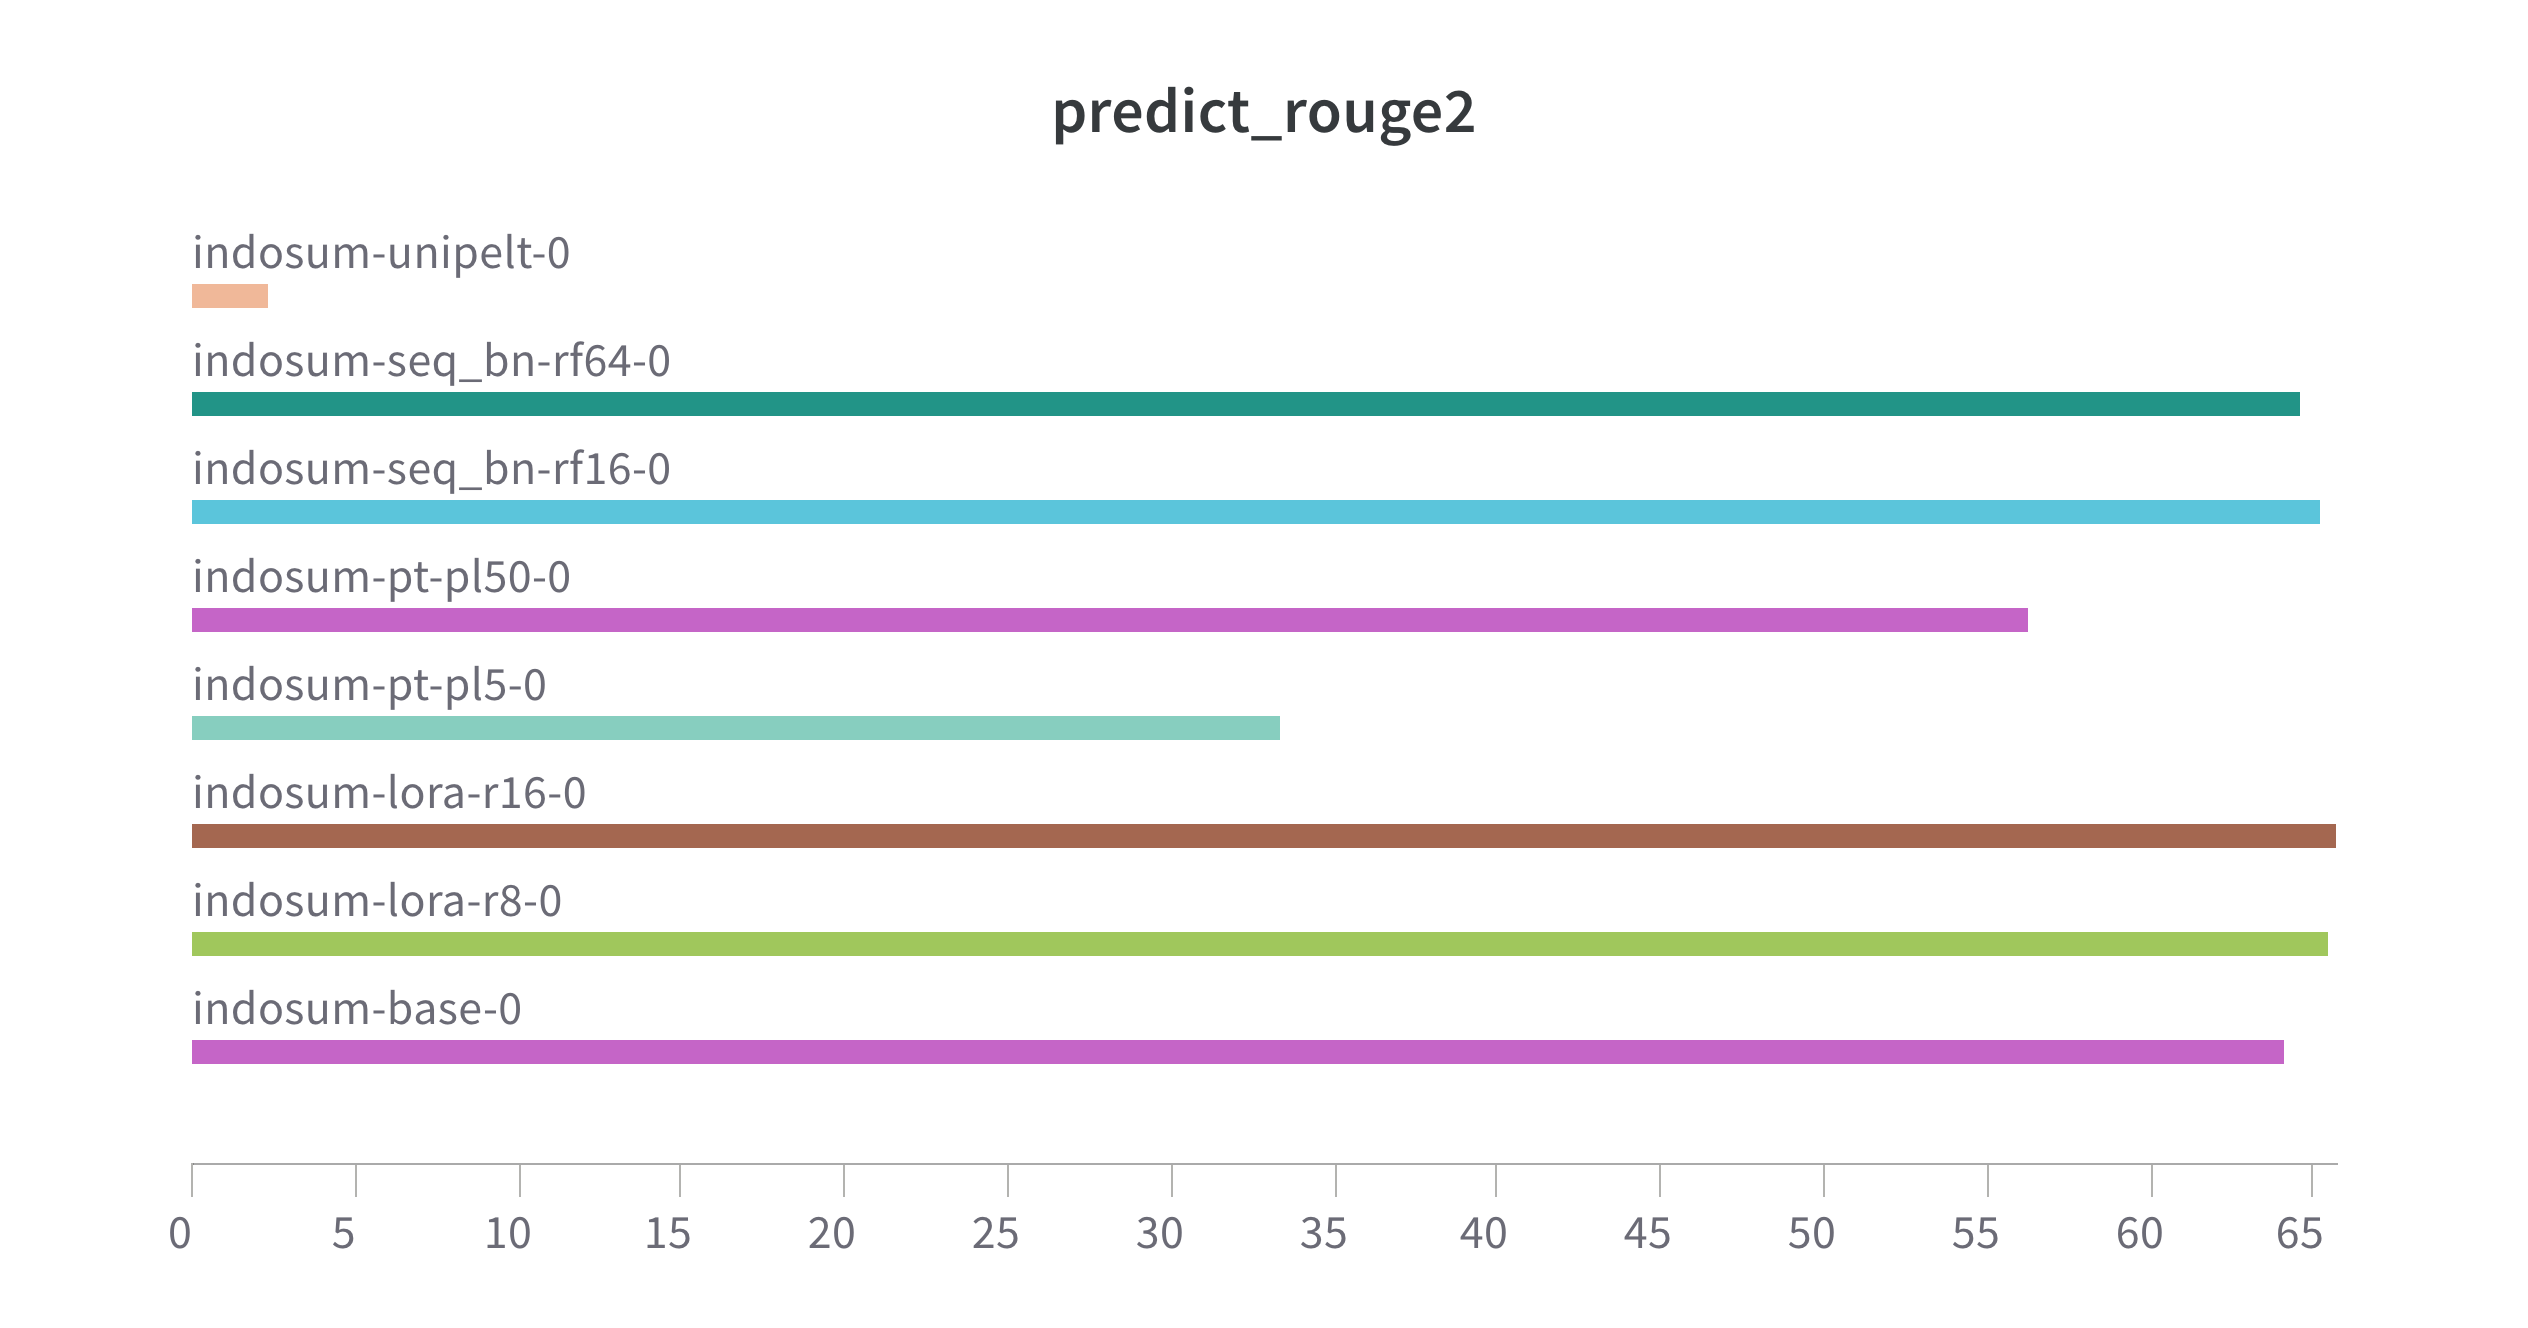
\includegraphics[width=\textwidth]{appendix/summ_pred_r2.png} \\
    \end{longtable}
    \caption{Hasil evaluasi dan prediksi ROUGE-2 tugas \textit{summarization}}
\end{figure}

\begin{figure}[h]
    \centering
    \begin{longtable}{c}
        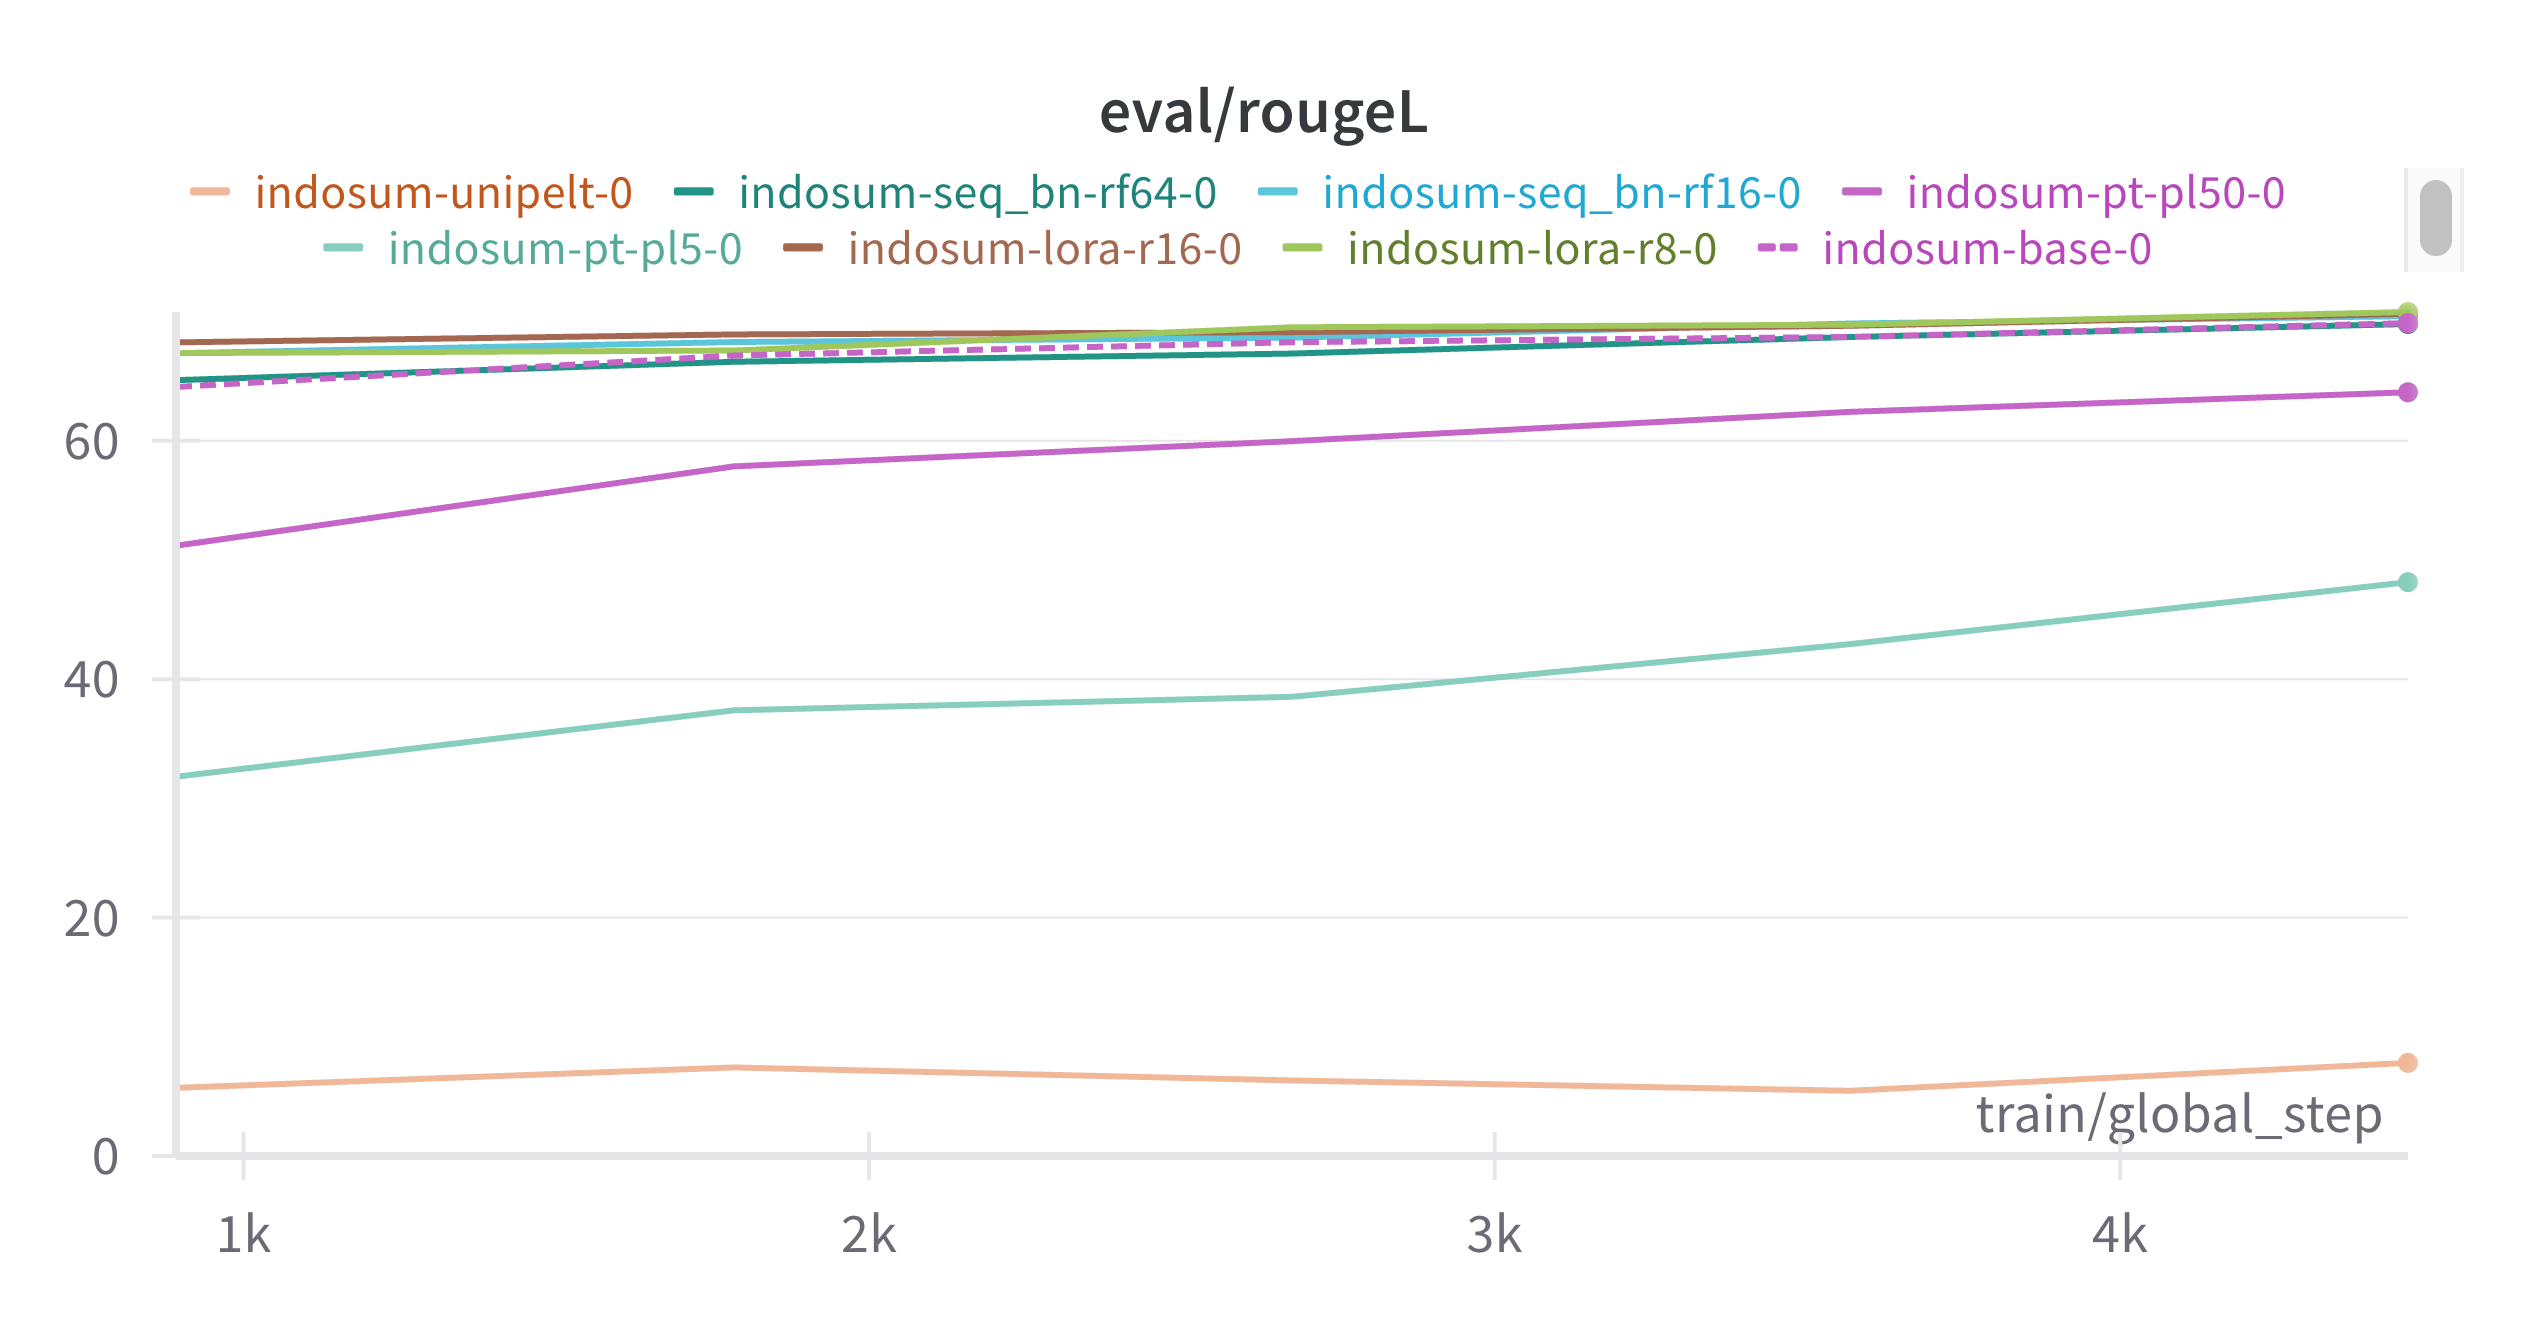
\includegraphics[width=\textwidth]{appendix/summ_eval_rl.png} \\
        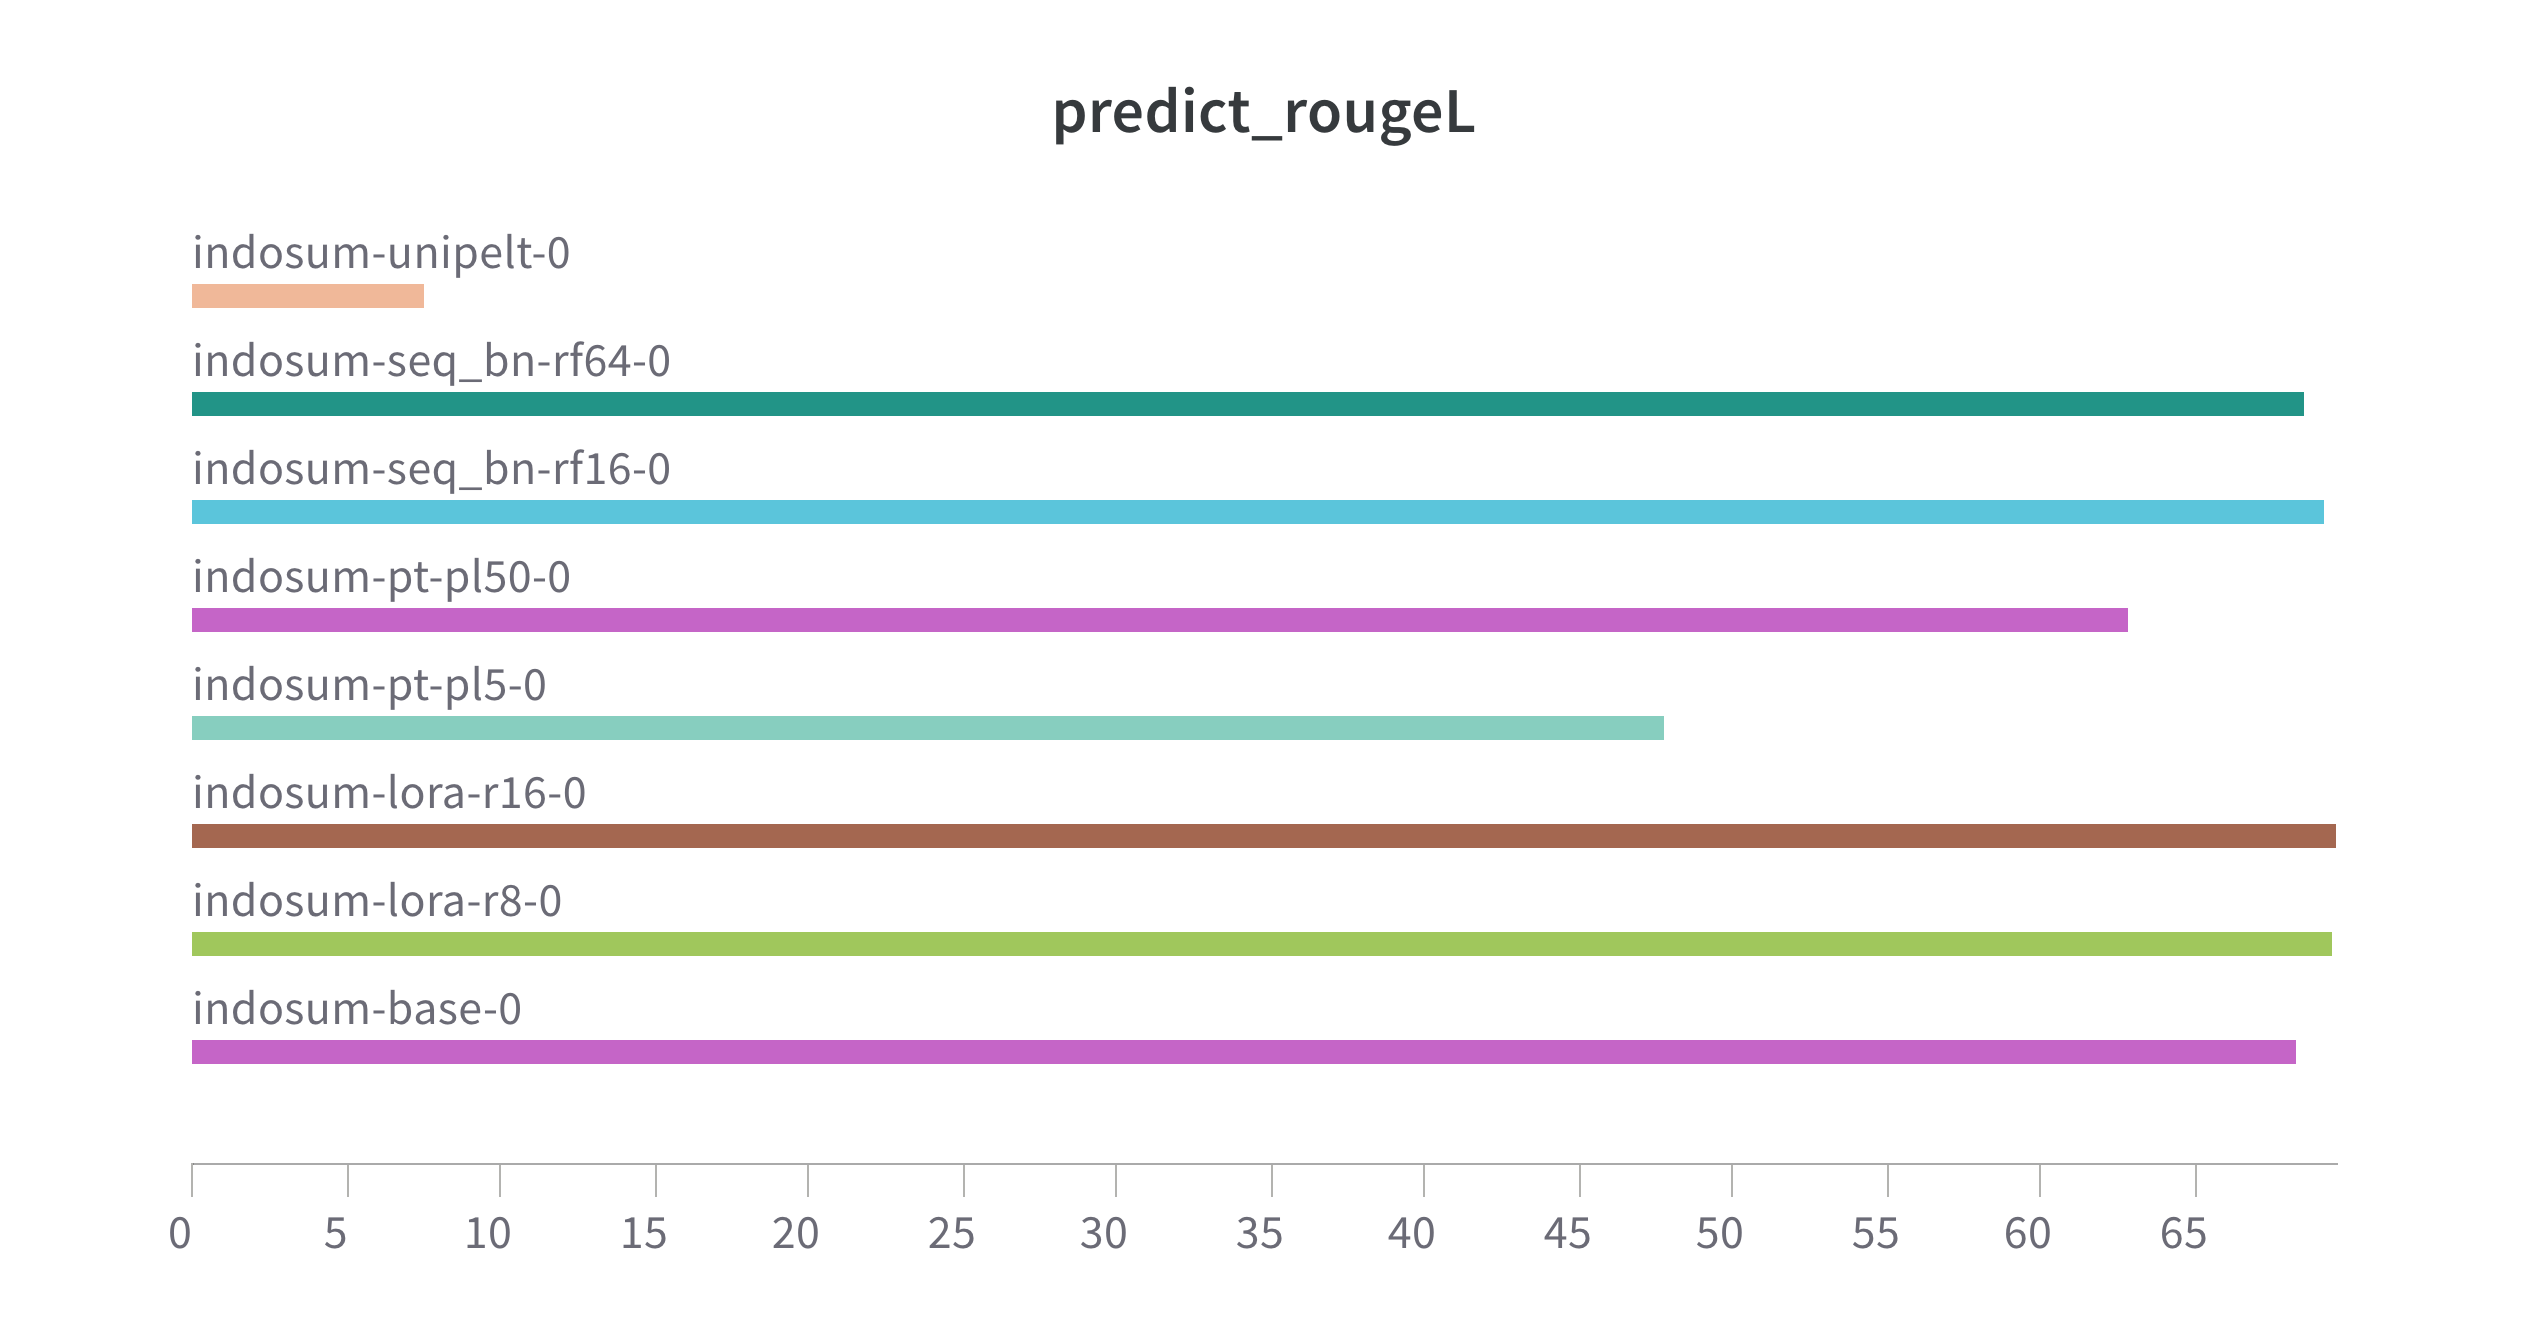
\includegraphics[width=\textwidth]{appendix/summ_pred_rl.png} \\
    \end{longtable}
    \caption{Hasil evaluasi dan prediksi ROUGE-L tugas \textit{summarization}} \end{figure}
